%% 
%% Copyright 2019-2020 Elsevier Ltd
%% 
%% This file is part of the 'CAS Bundle'.
%% --------------------------------------
%% 
%% It may be distributed under the conditions of the LaTeX Project Public
%% License, either version 1.2 of this license or (at your option) any
%% later version.  The latest version of this license is in
%%    http://www.latex-project.org/lppl.txt
%% and version 1.2 or later is part of all distributions of LaTeX
%% version 1999/12/01 or later.
%% 
%% The list of all files belonging to the 'CAS Bundle' is
%% given in the file `manifest.txt'.
%% 
%% Template article for cas-sc documentclass for 
%% double column output.

%\documentclass[a4paper,fleqn,longmktitle]{cas-sc}
%\documentclass[a4paper,fleqn,onecolumn]{cas-sc}

\documentclass[final]{article}


% if you need to pass options to natbib, use, e.g.:
%\PassOptionsToPackage{numbers}{natbib}
% before loading neurips_2022


% ready for submission
\usepackage{neurips_2022}



\usepackage[utf8]{inputenc} % allow utf-8 input
\usepackage[T1]{fontenc}    % use 8-bit T1 fonts
\usepackage{hyperref}       % hyperlinks
\usepackage{url}            % simple URL typesetting
\usepackage{booktabs}       % professional-quality tables
\usepackage{amsfonts}       % blackboard math symbols
\usepackage{nicefrac}       % compact symbols for 1/2, etc.
\usepackage{microtype}      % microtypography
\usepackage{xcolor}         % colors


%\usepackage[numbers]{natbib}
%\usepackage[authoryear]{natbib}
%\usepackage[authoryear,longnamesfirst]{natbib}
\usepackage{tikz}
\usetikzlibrary{positioning}
\usetikzlibrary{calc,through,backgrounds}
\usepackage{pgfplots} 
\pgfplotsset{compat=newest}
\usepgfplotslibrary{groupplots}
\usepgfplotslibrary{dateplot}
\usepackage{algpseudocode}
\usepackage{algorithm}
\usepackage[export]{adjustbox}
\usepackage{amsmath,amsfonts,amssymb}
\usepackage{siunitx}
\usepackage{tabularx}
\usepackage{tabulary}
\usepackage{booktabs}
\usepackage{makecell}
\usepackage{multirow}
\usepackage{array}
\usepackage{colortbl}
\usepackage{dcolumn}
\usepackage{stfloats}
\usepackage{xspace,xstring,footmisc}
\usepackage{longtable}
\usepackage[export]{adjustbox}
%\usepackage{cas-common}
%\usepackage{graphicx}
%\usepackage{array}
%%%Author definitions

%%
%%%%%%
%NOTACION
\newcommand{\vc}[1]{\mathbf{#1}}     %vectors (bold type)
\newcommand{\ma}[1]{\mathbf{#1}}     %vectors (bold type)

%%%%%%
%EDITION
\definecolor{mycolor}{cmyk}{1,0,1,0}
\definecolor{mycolor1}{rgb}{1.00000,0.50000,0.00000}%
\definecolor{mycolor2}{rgb}{0.00000,0.80000,1.00000}%
\definecolor{mycolor3}{rgb}{1.00000,0.00000,1.00000}%
\definecolor{mycolor4}{rgb}{0.45, 0.31, 0.59}%
\definecolor{mycolor5}{rgb}{0.6, 0.4, 0.8}
\definecolor{carnationpink}{rgb}{1.0, 0.65, 0.79}
\definecolor{auburn}{rgb}{0.43, 0.21, 0.1}



\begin{document}
\let\WriteBookmarks\relax
\def\floatpagepagefraction{1}
\def\textpagefraction{.001}

% Main title of the paper
\title{Thread Counting in Plain Weave for Old Paintings Using Semi-Supervised Regression Deep Learning Models}                      


\author{%
 A.Delgado \\
  Dep. Teoría de la Señal y Comunicaciones.\\
   ETSI. Universidad de Sevilla.\\
  Camino de los Descubrimientos sn\\
  Sevilla, 41092. Spain \\
%  \texttt{hippo@cs.cranberry-lemon.edu} \\
  % examples of more authors
   \AND
   Juan.~J.~Murillo-Fuentes\\
  Dep. Teoría de la Señal y Comunicaciones.\\
   ETSI. Universidad de Sevilla.\\
  Camino de los Descubrimientos sn\\
  Sevilla, 41092. Spain %\\
   \texttt{murillo@us.es} 
     \And
   Laura~Alba-Carcelén. \\
   Dep. Restauración y Documentación Técnica
   Museo Nacional del Prado \\
   Paseo del Prado s/n \\
   28914 Madrid. Spain
}

% Title footnote 1.
% eg: \tnotetext[1]{Title footnote text}
% \tnotetext[<tnote number>]{<tnote text>} 


\maketitle

% Here goes the abstract
\begin{abstract}
In this work, the authors develop regression approaches based on deep learning to perform thread density estimation for plain weave canvas analysis. Previous approaches were based on Fourier analysis, which is quite robust for some scenarios but fails in some others, in machine learning tools, that involve pre-labeling of the painting at hand, or the segmentation of thread crossing points, that provides good estimations in all scenarios with no need of pre-labeling. The segmentation approach is time-consuming as the estimation of the densities is performed after locating the crossing points. In this novel proposal, we avoid this step by computing the density of threads directly from the image with a regression deep learning model. We also incorporate some improvements in the initial preprocessing of the input image with an impact on the final error. Several models are proposed and analyzed to retain the best one. Furthermore, we further reduce the density estimation error by introducing a semi-supervised approach. The performance of our novel algorithm is analyzed with works by Ribera, Velázquez, and Poussin where we compare our results to the ones of previous approaches. Finally, the method is put into practice to support the change of authorship or a masterpiece at the Museo del Prado.

\end{abstract}

% Use if graphical abstract is present
% \begin{graphicalabstract}
% \includegraphics{figs/grabs.pdf}
% \end{graphicalabstract}

%% Research highlights
%\begin{highlights}
%\item Research highlights item 1
%\item Research highlights item 2
%\item Research highlights item 3
%\end{highlights}
%\clearpage
% Keywords
% Each keyword is seperated by \sep
%\begin{keywords}
%X-ray processing \sep Canvas weave \sep Thread Counting \sep Artificial Neural Networks \sep Regression \sep Inception \sep VGG \sep Residual Learning
%\end{keywords}

\maketitle


 \section{Introduction}\label{sec:intro}
\subsection{Interest in Fabric analysis}
In the forensic study of a painting, the analysis of the fabric plays an important role. In particular, the following features are checked \cite{Alba21}:
\begin{itemize}  \setlength\itemsep{.1em}
\item The type of fabric: plain wave, twill, or satin.
\item The fabric material: cotton, linen, silk, ...
\item The number of threads per centimeter in both vertical and horizontal orientation (density of threads), especially in plain weave.
\item The angle deviations of the threads with respect to the horizontal and vertical axis.
\end{itemize}

%The angle deviations All these features allow conservators to determine if the fabric remains intact and keeps its original size or, if on the contrary, it has undergone modifications or some pieces are missing. It is therefore remarkable the information that the study of the canvas provides to conservators when they have to attribute hitherto anonymous artworks. 

In this work, we focus on the plain weave and its thread density. Plain weave\footnote{Also known as taffeta, tabby, or calico weave.} fabrics are predominant. They are the support for a vast number of paintings thanks to their good compromise between robustness and simplicity \cite{Vanderlip80}. Plain weave is characterized by an intertwining of the vertical threads with the horizontal ones, see Fig. \ref{fig:Taffeta}.a. A set of threads are arranged in parallel on a loom from back to front before starting to weave. These threads are called the warp. The separation between the warp threads follows a deterministic pattern that is determined by their placement on the loom. On the other hand, the weaver passes another thread orthogonally to the warp from one side to the other, tightens it, and passes it back, intertwined. This other thread is the weft. Since weft tightening follows a manual process, %we can expect a certain randomness, and 
the distance between weft yarns can be usually modeled by a Gaussian random variable. This crossing of warp and weft threads forms a balanced and robust fabric \cite{Alba21,Simois18}. In fabric analysis with image processing and computer vision, the X-ray of the canvas is used because usually the fabric can not be directly observed as a quite extended technique to reinforce the support of the painting is to stick a piece of cloth on the back. The intensity of each pixel in the image of the X-ray plate depends on the amount of paint and primer in that area, and the presence of wood stretcher, nails, or other opaque artifacts, etc. In Fig. \ref{fig:Taffeta}.b we include some examples of X-ray plates from different canvases using plain weave.

%Thanks to the characteristics of the canvas, a painting can be located in a specific place and time and, from there, an attribution to an author can be made through these data or through a comparison with the canvas of other paintings \cite{Alba21}. In this paper we are focusing on one of the commented features: the density of threads per cm. Specifically, we present a new method to obtain the number of threads in patches of 1cm side. This method is faster and more reliable than previous works in literature.


\begin{figure}[htbp]
\centering
\begin{tabular}{cc}
 \includegraphics[width=3.5cm]{tafetanML.png} &\includegraphics[width=4.0cm]{flavorsReg.png}\\
 (a) & (b) 
 \end{tabular}
\caption{In (a) an sketch of plain weave with warp and weft yarns in weaving as described in \cite{Barlow1878} and in (b) patches of 1 cm side from X-ray plates of paintings using plain weave. 
% Image from Wikipedia, authors Ryj, PKM.
} \label{fig:Taffeta}
\end{figure}

Because the separation of the threads in plain weave is not regular and depends on the manufacturing and the loom, if we find the same pattern in two canvases we can conclude that both come from the same bolt. This is critical to date a canvas or even to change its authorship, by comparison to other well-studied paintings. Traditionally, curators analyzed the fabric of the canvas at some locations, by counting the number of vertical and horizontal threads in 1 cm side squares. However, this provided a rough estimation of the mean value of thread densities. If densities were different enough for a couple of canvases, the curator concluded that they did not share the fabric of a roll. Otherwise, curators could not rule out the possibility of both paintings using the same cloth. With the introduction of automatic thread counting \cite{Johnson2010,Johnson2013} the curators not only avoid the tedious task of counting but they have access to a map of densities for vertical thread throughout the painting, and another for horizontal ones. Angle deviation can also be estimated. By matching these maps, usually depicted using colormaps, the curator concludes on the fabrics of two or more canvases. 

  
%When studying a canvas, the relationship between the weft and the warp give us a lot of information. Because of this, the counting of threads per centimeter in both directions (vertical and horizontal) is used as a fundamental characteristic of study \cite{Alba21,Simois18}. So, we are interested in knowing the number of vertical and horizontal threads in each canvas fragment of 1 cm side. Repeating this calculus around the whole painting we are able to generate two colour maps that represent the density of threads in each location on the plate. These maps will be called density maps. When making comparatives between different paintings, density maps can be very useful. In fact, we know that all canvases made from the same warp roll will have the same thread densities in the warp direction, so a match between the warp density maps should be found.


\subsection{Motivation and Contributions}

In Fig. \ref{fig:Taffeta}.b we include several examples of patches, of 1 cm sides, to evidence that while counting threads may be an easy task in some cases, it can be really hard in others. Poor resolution, noise from the painting itself or cracks, distortions such as rotations, or a high density of prime make it difficult to count the number of threads in any scenario. We have recently proposed a method for thread density estimation based on deep learning (DL) \cite{AE86,Goodfellow2016} by segmenting crossing points \cite{Bejarano2022a,Bejarano2022b,Bejarano2023}. 
 %However, no further equalization was introduced. 
Segmentation of crossing points based on DL presented good results regardless of the impairments present in the input image. However, it is needed the estimation of the densities from the segmentation result, computed in posterior processing. Furthermore, in the segmentation DL paradigm, it is quite difficult to link the segmentation result with the error in posterior thread counting. In this work, we face the direct estimation of the densities by using a regression model. On the one hand, we remove the processing after the segmentation, reducing computational running time. On the other, we use as training loss function the error in the estimation of the thread density, providing a more accurate result. 

One of the major difficulties of the DL is the need for labeled samples in the training stage. This training is run once and then the weights of the model are fixed and ready to be used in the analysis of any painting. A rich and wide set of samples, covering different qualities of fabrics, ranges of thread densities, and noises are needed. But the labeling stage is not only time-consuming but quite hard to accomplish for high-density thread fabrics and noisy images. To create a large dataset, data augmentation (DA) was exploited in \cite{DA2019}, where we cropped areas of labeled samples to generate inputs. Besides, we further augmented the data set by randomly rotating the result of the cropping. Also, the images were pre-processed to get a wide range of intensity values of pixels around a fixed value. Filtering with kernels of fixed size was performed in this step.


%Borrowing from the segmentation approach in  \cite{Bejarano2023} 
We propose a novel algorithm that incorporates three major improvements.
%
First, we avoid the post-processing of the segmentation result by resorting to regression and forcing the DL model to directly compute the thread density itself. Hence, the output of the network would be the number of vertical threads per cm in that image. Note that to obtain the horizontal density of threads, the input image is rotated 90$^\circ$. We develop and analyze different models to retain the one with the best performance where we perform an optimized search \cite{Snoek12,Omalley19} to set their hyperparameters.

Second, we deeply review the data generation process in \cite{DA2019}. In the pre-processing step, the size of the kernel is not fixed but automatically adapted to the image, depending on a rough estimation of the thread densities. Also, equalization is incorporated. In the DA, we limited the random rotation applied to some of the images and increased the number of images from 21,540 to 30,156 by also cropping central parts of the labeled samples. 

Third, to improve the results in scenarios where the FT provides accurate estimates we introduce semi-supervised training. When processing a new full painting, inputs for which both the DL and the FT provide similar density estimates are incorporated into the training dataset. 

These improvements reduce the error in the estimation of thread densities. Besides, the first one reduces the running time. We include several experiments to compare the outcome of our approach to the one of previous proposals. Finally, we use the new method to report new results on the forensic analysis of a pair of paintings at the Museo del Prado, which helped the curators to change the authorship of one of them. 

%In this paper we present an improvement of the last work mentioned. In this sense, we present a new DL approach in order to obtain the density of threads using Deep Learning models. Specifically, we pretend to unify the process using only Deep Learning. This new approach would avoid the use of the mentioned image-processing algorithms that were used to binarize the segmented image and to estimate the number of threads. These tasks will be performed by the neural network intrinsically. Besides, a tool to tune some parameters and hyperparameters of the ANN will be used to design the optimal architecture. All this points contribute to improve the execution time when density maps from big paintins are being generated. In addition, we get more accurate results because the image-processing algorithms were the most responsable of the error in the previous segmentation approach.

%We will design a new neural network to perform a regression with the extracted features from each image. In this way, the output of the network would be the number of vertical threads per cm in that image. In this paper we will present different models that provides the number of vertical threads in the image, that is, the vertical density of threads per cm. To obtain the horizontal density of threads, it is enough to rotate 90$^\circ$ the input image. We will use the same database described in \cite{Bejarano2023}. In short, we have 21540 images of 200x200 pixels size, all of them having an adjusted resolution of 200 px/cm resolution. These images were extracted from 36 paintings from Museo Nacional del Prado. The paintings were selected to be representative of several densities (in the range 6 to 23 threads per cm), different resolutions of the image and noise conditions. This encompasses the usual densities found in canvases. The process of prepraring the dataset and the labeling stage can be consulted in full detail in \cite{Bejarano2023}.

In summary, the main contributions of the paper are as follows:

\begin{itemize}\setlength\itemsep{.1em}
\item Novel DL models based on regression to directly estimate thread densities for fabrics in old paintings, avoiding cumbersome time-consuming signal processing approaches of previous methods. %This new approach reduces the time needed to obtain the density maps of whole paintings. %This is especially noticeable when dealing with big X-ray plates.
\item Optimized search of the hyperparameters of the proposed models and detailed comparison of the performance of the proposed approaches and the segmentation-based DL method. \cite{Bejarano2023}.
\item Improvements in the DA stage: the limitation of the maximum random rotations and the inclusion of more images from labeled samples to enlarge the dataset.% from 21,540 to 30,156 images.
\item New algorithm to adaptively select the kernel size in the preprocessing approach, adjusting it to the thread densities and enhancing the contrast of the input images. 
\item Using equalization as the last step of the pre-processing to further improve the performance of the approach.
\item A semi-supervised training that automatically includes new labeled samples, those with similar results of the regression DL and the FT approaches.
\item Application of the method to the analysis of masterworks by Velázquez, Poussin, and Ribera at El Museo N. del Prado and The National Gallery, to illustrate the performance of the method compared to the FT, the thread level canvas analysis in \cite{Maaten15} and segmentation DL \cite{Bejarano2023} algorithms.
\item Results on the forensic study that helped to change the authorship of a masterpiece attributed to Rizi at El Museo Nacional del Prado. 

\end{itemize}


\section{Related works}
In the literature, we find three different main techniques for the threads density estimation. Namely, those based on frequency analysis, feature extraction followed by machine learning, and DL.

\subsection{Frequency Analysis}
In \cite{Escofet2001,Johnson2013,Simois18} a theoretical framework is defined in order to model a fabric through a frequency analysis based on the 2D Fourier transform (FT). In the frequency domain, there is a repetition pattern that can be described as a quasi-periodic function in both vertical and horizontal dimensions. The maximum values of this pattern are related to the thread densities of the plain weave. In \cite{Johnson2010,Johnson2013}, this idea was exploited to obtain the first thread counting maps, by applying the 2D discrete FT to 1 cm side square images all over the X-ray plate and finding the maxima. The main advantage of this approach is that it is an unsupervised method, i.e., it does not need any labeling. Besides, it is usually a very robust tool in the presence of noise, such as the painting itself, and artifacts in the X-ray such as nails or stretchers. It also works in poor contrast scenarios. For these reasons, in scenarios where we have a quite uniform warp-weft pattern of threads, the FT provides quite a good result. The FT has been widely used in many studies in the last decade. However, in cases where we do not have a clear and periodic pattern the FT is not useful. In \cite{Bejarano2023} it is reported that the FT fails whenever we have different distances between nearby threads, the width of the threads varies, or the warp is tighter than the weft. In the last case, we clearly observe the warp threads and the weft is observed as a widening of the threads at the crossing points.  

%For all these reasons, the discrete FT in two dimensions (2D-DFT) is a powerful tool to obtain the density maps.

%Likewise, a method to compare the obtained density maps and match them is presented, so that it can be concluded if two canvases were obtained from the same loom. In \cite{Simois18,Velasco22}, the previous work is extended specifying for various types of fabrics. The reason why the authors resort to frequency studies of the X-ray plate is that the threads form a repeating pattern on the plate. 

Another interesting work is the one presented in \cite{Simois18} based on the 
%The authors found some limitations when FT is used to obtain the density maps. Mainly, it is argued that the frequency study of fabrics does not work well when if the fabrics are damaged. In fact, it is not uncommon to find old paintings in which a piece of the original canvas is missing or irregularities have appeared as a result of the passage of time. Due to this, 
%It is proposed to resort to the 
power spectral density (PSD). The maximum levels of the PSD exhibit a pattern that characterizes the structure of the fabric, allowing different paintings to be compared. PSD can be viewed as a fingerprint of the canvas as for fabrics with the same thread densities, relevant differences can be observed in the frequency domain. Based on \cite{Simois18}, the Aracne software \cite{Murillo14} was developed. However, it cannot be used to match the warp or weft pattern between canvases.%, and it is the preferred and most conclusive clue of paintings sharing the same bolt. %The averaging helps to reduce the effect of deteriorated parts of the frame. In addition, from the PSD they also extract the mean thread count of the whole painting in both directions. In summary, although the PSD is not useful for building thread density maps, it is a great alternative for studying and classifying works due to the number of characteristics that can be extracted from it. 

\subsubsection{Feature Extraction Approach}

Another approach that has been proposed to study the thread density in canvases is based on feature extraction and machine learning \cite{Maaten15}. Compared to the frequency analysis, in \cite{Maaten15} the authors resort to the spatial domain to find every crossing point in the warp-weft pattern. The approach, presented as an automatic thread-level canvas analysis tool, hereafter denoted by ATCA, extracts histograms-of-oriented-gradient features that are the input to machine learning methods such as support vector machine and Bayesian logistic regression classifiers that determines if a location in the images is a crossing point or not. By applying the approach through every pixel, it is possible to generate density maps.

%The authors expresses that more than having the number of threads in a certain area, it would be interesting to identify each thread separately and measure the distance and angles between the different threads found in the X-ray of the fabric. A new method of study is proposed at the thread level (not at the patch level or full painting level) using a Machine Learning (ML) SVM-based model that locates the crossing points between vertical and horizontal threads. Once the model is trained, it can be used to detect such crossing points throughout the entire plate. However, t

This method exhibits a major drawback, it is necessary to label a large number of crossing points in the images for the to-be-analyzed X-ray plates. This is really cumbersome for the practitioner. This labeling is not trivial, since in many cases threads are not even well observed. Besides, the method depends on a set of parameters whose optimal values depend on the image itself. While some of them are automatically computed, others might need manual adjustment.


\subsubsection{Deep Learning}
Algorithms based on artificial neural networks have been applied to several problems in art. In \cite{Sizyakin20} convolutional neural networks (CNN) were used for crack detection. A CNN was also applied to the automatic classification of paintings \cite{Roberto2020}. In \cite{Pu2020} auto-encoders (AE) were used for image separation. In \cite{Zou21} DL was applied for the virtual restoration of colored paintings. Segmentation through U-Net \cite{Unet15} and AE \cite{AE86,Goodfellow2016} was applied to image restoration by inpainting. 

In the analysis of plain weave fabrics, crossing points can be detected using segmentation based on DL approaches. This is the idea of the method in \cite{Bejarano2022a,Bejarano2022b,Bejarano2023}. A U-Net \cite{Unet15} based model is proposed to locate crossing points in a 1 cm side square input image. Then signal processing is used to estimate the average distance between crossing points. The process is repeated for locations along the canvas to get the density maps. 

In the training stage, a large number of labeled samples were needed. Overall 239 samples of 1.5 cm side images were labeled and preprocessed. Then, 21,540  square images of 1 cm side were generated by cropping these samples and using DA. Although this process is cumbersome, it is performed just once. The curator can later use the trained tool with no additional labeling of the scanned X-ray plate at hand. Hence, compared to the ATCA method, this method avoids any further labeling.
 The preprocessing involves double filtering to reduce the difference in the mean of the input images and increase their contrasts. The kernel size of the involved filters was fixed, regardless of the thread density values. No equalization was applied. 
The algorithm provided good estimates where FT methods fail. In other cases, the FT presented slightly better results. 

%Image processing has been applied to the study of priceless paintings \cite{Barni05}. The removal of canvas was studied in \cite{Cornelis12,Cornelis17,Deligiannis2017}  where the fabric was considered as a noise component superimposed on the painting artwork. Crack detection and inpainting was developed in \cite{Cornelis13} and a cradle removal approach in \cite{Yin14}. Style, authentication and forgery analysis was also accomplished by means of  the brushwork analysis \cite{Johnson08}, advanced correlation filters \cite{Buchana2016} or contourlet transform \cite{Jacobsen13}, where style is studied \cite{Li2004}. Chemical element extraction from macro X-ray has also received a remarkable interest \cite{Yan2021}. 
%Image separation was also faced exploiting AE \cite{Pu2020}.
 
%To the best of our acknowledgement there is only a previous work that uses Deep Learning (DL) to generate the density maps from X-ray plates of old paintings \cite{Bejarano2022a,Bejarano2022b,Bejarano2023}. This work intended to improve the results in some situations where frequency analysis don't work well, as well as to provide a method that does not require labeling new samples for each plate to be processed. The authors designed an artificial neural network to segment the cross points in 1cm side crops from X-ray plates of old paintings. An encoder-decoder architecture (U-Net) was designed follows the Inception paradigm and different variants of that network were tested. Later, they obtain the density of threads per cm from the segmented cross points using some image-processing algorithms. Said algorithms are used to binarize the segmentation image obtained as output of the network and to obtain the density of threads per cm by averaging the distance between the segmented points. The presented results are quite good and some interesting conclusions are reached when density maps are compared for different paintings.

\section{Data Generation}\label{sec:DG}

The dataset used, the same one as in \cite{Bejarano2023}, has 239 labeled samples of $1.5$ cm side from 36 selected paintings from the Museo Nacional del Prado (MNP). Canvases from Rubens, Velázquez, Lorena, Swanevelt, Dughet, Poussin, Both, Lemaire, and Ribera, among others, were included in the dataset. The fabrics of these paintings have several densities in the range of 6 to 23 threads per cm (thr/cm), different resolutions of the image, and several noise conditions. This encompasses the usual densities found in canvases, see for example the analysis of thread densities in \cite{Vanderlip80} for French painting. %within the 17th-20th centuries period for French 44 artists.%, the densities of the threads were in the range 6-23.3 thr/cm. For the 17th and 18th this range reduces to 8.6-20 thr/cm.
%
The models later presented will be trained and tested with this dataset, but the pre-processing and DA are modified as follows.

%\subsection{Pre-Processing}

%\subsection{Added Improvements}
%Once we have checked that the regression approach provides similar results that the segmentation method but it is faster more efficient, we try to improve the results achieved. In order to get the improvement desired, we have introduced some variants in how the database is built and in how the model is training. Specifically, the improvements added are:
\subsection{Adaptive Kernel Size}
We have adapted the pre-processing in \cite{Bejarano2023} of the samples from the X-ray plate to better cleanse them. When performing the cropping, mean and local standard deviation filters were applied (see \cite{Bejarano2023} for a full description). Both filters had fixed sizes. We found that images high a better contrast could be obtained by adapting the kernel sizes to the mean fabric thread density. For this reason, we propose to  apply a dynamic window based on the average distance between threads of each fabric, which can be quickly extracted with a coarse frequency analysis of the whole X-ray plate. %In this way, we are going to train the network with the same crops but with a cleaner appearance, since dynamic windowing provides images where the threads are easier to see, especially in extreme cases of very high or very low counts.
 In Fig. \ref{fig:window}.a we include a pre-processed  sample with fixed size kernel and in Fig. \ref{fig:window}.b we have the same sample pre-processed with adaptive kernel size. We highlighted some areas where a better contrast is observed, i.e., it is easier to distinguish crossing points from dark areas between threads. We also zoomed one of them.
 
 The algorithm to estimate the size of the kernel to pre-process the image is described in Alg. \ref{alg:VW}. This method is run twice, with an initial value $k_0=21$ and then with the result of this first iteration. The linear regression in the algorithm was adjusted to provide the best kernel size from the estimation of the thread densities, based on several previous results processing canvases.
 
 
 %%%%%%%%%%%%%%%%%%%
 
\begin{algorithm}
\caption{Kernel Size Estimation}\label{alg:VW}
%\hspace*{\algorithmicindent} 
\textbf{Input:} Scanned X-ray plate image and initial kernel width $k_0$.
\begin{algorithmic}[1]
\State Pre-process the X-ray with kernel width of $k_0$.
\State Rough estimation of the thread densities with FT of 512 points by sampling $1 \times 1$ cm images from the X-ray plate every 7-15 cm, depending on the canvas size.
\State Estimate the histogram for the vertical and horizontal densities, typically with $300$ bins, and retain the largest values above the mode divided by 1.5. Average the horizontal and vertical values, $t$.
%\State Cuando ha recorrido toda la placa se calcula el histograma de los conteos V y de los H por separado, con 300 bins. De todos los conteos que son mayores que la moda / 1.5, nos quedamos el bin de más a la derecha. Esto lo hago porque hay algunas (pocas) ocasiones donde el histograma sale bimodal, y el modo de la izquierda es ruido de la FT que cuenta de menos, nunca he visto de cuente de más. De esta forma nos quedamos con el conteo “correcto”.
%\State Teniendo ya un conteo vertical y otro horizontal, obtenemos la media de ambos y ese es el valor de conteo de la placa. Ahora hay que ver qué ventana corresponde a ese valor de conteo. Para "traducir" el valor de conteo a tamaño de ventana he usado una regresión lineal de Scikit. La regresión lineal es un modelo de ML que hay que entrenar, para ello fijé experimentalmente una serie de valores: para las placas de entrenamiento y validación determiné experimentalmente el valor de conteo promedio con FT y el valor de ventana con el que el pre procesado tenía mejor apariencia. Además, a la vista de que la red aprende mejor con ventana fija que con ventana variable, tuve en consideración cambiar los valores de ventana en los casos de conteos más extremos, mientras que en placas con un conteo medio intenté que todas tuvieran la misma ventana. Con esas parejas de conteo-ventana entreno el modelo de ML que luego uso para predecir el valor de la ventana dado el conteo.
\State Estimate the pre-processing kernel size by applying the following linear regression, 
\begin{equation}
k = -0.90 \cdot t + 37.05
\end{equation}
Then $k$ is first rounded to the nearest value to 14.5, and then to the lowest odd number. 
%Ahora se le pasa el valor de conteo de la placa calculado antes con la FT y obtengo el valor de la ventana según la regresión lineal. Este valor de la ventana es un valor en punto flotante, hay que traducirlo a un número entero impar. Si el valor del conteo es mayor de 14.5 se toma como ventana el entero inferior (floor) y si es menor de 14.5 el entero superior (ceil). Para que sea impar hacemos la siguiente conversión:   $ventana = ventana // 2 * 2 + 1$. El dividir el rango de conteo en 14.5 es porque es aproximadamente la mitad del mismo, la idea es tomar el impar más alto si el conteo es bajo y viceversa.
%\State Con esto ya tenemos el valor impar que queremos. Falta por sacar el margen en función de la ventana. El margen debe ser al menos el doble de la mitad ventana porque se hacen dos filtrados (media y std). Para ello tomamos un margen auxiliar como: $margen_aux = ventana // 2 * 2$
%\State Y a este valor le sumamos un término adicional para tener margen suficiente y no quedarnos cortos en ninguna situación. Ese término se ha tomado como: la sexta parte del margen auxiliar anterior: $Margen = margen_aux + margen_aux //6 $
%\State De esta forma tomamos un margen de seguridad extra en función de la ventana, si la ventana es mayor se deja un poco más de margen que si la ventana es pequeña.
%\State Una ves estimado el valor de la ventana y el margen, repetimos el procedimiento de estimación de ventana y margen usando ahora los valores de ventana y margen calculados para el preprocesado de la FT. Así conseguimos una estimación algo más precisa. El único caso en que este proceso no se realiza dos veces es si, tras la primera estimación, el valor de ventaja sigue siendo 21. En ese caso finaliza el proceso sin la segunda estimación 
\\
\textbf{Output:} $k$
\end{algorithmic}
\end{algorithm} 
 

\begin{figure}[htb]
\centering
\begin{tabular}{cccc}
 \includegraphics[width=3.8cm]{oldZoom.png}& 
 \includegraphics[width=3.8cm]{windowZoom.png}\\
(a) & (b) 
\end{tabular}
\caption{Input image obtained with (a) fixed window size and (b) dynamic window size. We have highlighted some areas and one of them has been zoomed, where after using adaptive kernel size the contrast of the image has been improved. %Crossing points are better observed in these areas.
} \label{fig:window}
\end{figure}

\subsection{Equalization}
We include also an off-the-shelf equalization approach. We estimate the histogram, $h(x)$, for the gray levels of the input image, normalize it to sum 255 and compute its integral, $h'(x)$, and use the result as a look-up table. For a given input value, $x$, the output yields $y=h'(x)$.



\subsection{Rotations}
 The fabric of the canvases is usually distorted in some areas. In fact, along the stretchers, the fabric bends due to the tightness around the nails. In other areas of the canvas, the threads are not perfectly arranged vertically or horizontally; in some areas, the deviations can be severe. We include randomly rotated images in the data set to allow the model to learn the densities in rotated scenarios. However, we found that the maximum allowed rotations were larger than needed, and the model parameters were biased towards angle deviations not found in practice.  To avoid this bias we limited the maximum random rotations applied to half the maximum in \cite{Bejarano2023}. Hence, random rotations applied in the DA vary in the ranges [-6$^\circ$, -4$^\circ$], [-3.5$^\circ$, -1$^\circ$], [1$^\circ$, 3.5$^\circ$] and [4$^\circ$, 6$^\circ$]. 
 
\subsection{ Increasing the Dataset }
 The DA has also been modified in order to get more input images for every $1.5 \times 1.5$ cm labeled sample. Previously, in \cite{Bejarano2023} 30 samples were extracted from each sample. These images were mainly taken from areas in the corners of the labeled samples. Now, we add the cropping of the central regions given by the (50:250, 50:250), (65:265, 65:265), (35:235, 35:235), and (80:280, 80:280) pixels. These images are cropped from the original sample and the vertically and horizontally flipped versions (see \cite{Bejarano2023} for further details). In summary, now we get 42 images of $1 \times 1$ cm for every labeled sample, 40\% more than in \cite{Bejarano2023}. No randomly rotated versions of these images are included. Therefore, the ratio of the number of randomly rotated images to the overall number of images decreases. The number of images in the dataset is increased to 30,156.

%
%
%\item The last improvement consisted of adding a learning rate decay to stabilize the training. We could see that about 120 epochs were needed for the training to stabilize and, from there, the training became somewhat noisy, moving around the optimum. Because of this, we decided to implement a learning rate decay to reduce this value as the epochs progress. In this way, we favor a more leisurely and stable learning. The learning rate decay used followed the expression:
%\begin{equation}
%\text{Learning Rate} = \text{LR} * \frac{1}{1 + \frac{\text{epoch}}{10}}
%\end{equation}
%where LR is the inital learning rate value. It was set to $1.6*10^{-3}$.
%\end{itemize}
%
%The training of all the regression models presented before were repeated incorporing all the mentioned improvements.
%

\section{Regression DL Models} \label{sec:DL}

We designed four DL models to perform regression, providing the vertical density of threads per cm. All models follow the inception paradigm as in \cite{Bejarano2023} it was shown to be useful when dealing with images of different densities of threads. By applying the inception paradigm, we have convolutional kernels of several sizes in the same layer:  $3\times 3$, $5\times 5$, and $7\times 7$, see Fig. \ref{fig:Inception}. The results of the convolutions are concatenated at the output. Then, batch normalization is performed followed by a ReLU activation function. This will be used as a central block in the models below, represented by horizontal arrows in the schemes. The number above the horizontal arrows indicates the number of kernels used for each size. Hence the number of resulting features will be this number multiplied by 3. The rectangular prisms indicate the set of features at that point between layers. The number below the prisms are of the form $width \times height \times features$. All vertical arrows but the last two of them at the bottom denote a 2D max-pooling layer. The penultimate arrow indicates a flattening and the last one denotes a set of dense layers.

\begin{figure}[htbp]
\centering
 \includegraphics[width=7.7cm]{Inception2.pdf}
\caption{Inception block: $3\times3$, $5\times5$, and $7\times7$ kernels are convolved with the input at the same depth, as many times as given by the number of filters parameter, $n_i$. The results of these convolutions are concatenated.} \label{fig:Inception}
\end{figure}

\subsection{Labeling}

The data generation follows the procedure in \cite{Bejarano2023} with the modifications described in Section \ref{sec:DG} and an extra step to generate the labels for regression. 
While for the segmentation approach the label is an image with the intersection of the annotations for vertical and horizontal threads, for regression we need the density of vertical threads. The density of horizontal threads will be obtained by using the same model with 90$^\circ$ rotated images. Therefore, in the dataset, every image will be also included after applying a 90$^\circ$ rotation. For all of them, we need to estimate the density of vertical threads. 
%For the regression task the label corresponding to each image is the vertical density of threads. In this case we do not need the segmented image as a label. 
To compute the corresponding density of vertical threads for every image, we use the spatial counting (SC) approach developed in \cite{Bejarano2023} to estimate the thread density after the output of the segmentation DL models. At this point, it is important to remark that the SC algorithm is used just in the dataset generation in the training of the models but not later in the processing of a canvas, where the regression DL model directly provides the value of the thread density.
%. , it is possible to obtain the density of vertical threads from these labeled images. Reference \cite{Bejarano2023} can be consulted for more details on the labeling stage and spatial counting algorithm. Emphasize that in this case the spatial count is used to obtain the labels for training, not during the process of estimating the density of threads per cm.

The dataset is divided into three subsets: training, validation, and testing. Instances from the same canvas are included just in one of these subsets. The input test dataset is generated as described in \cite{Bejarano2023}, then duplicated after a 90$^\circ$ rotation. Labels were generated by using SC. 
The test subset is not used in the training stage or to select the model or hyperparameters, but just to analyze the final results.
%
We next propose four models. We later train and analyze them, to retain the one with the best performance. 

\subsection{Inception U-Net Pre-Trained Encoder}\label{ssec:RegUnet}
In this model we use a first set of layers corresponding to the pre-trained encoder from the Inc-Dice model in \cite{Bejarano2023}, a model exploiting the U-Net architecture and the inception paradigm. The output of these layers encodes the information to later locate the crossing points in the decoder. But as we need the estimation of the thread densities, we replace the decoder part of the U-Net with a fully connected (FC) network to perform regression, see Fig. \ref{fig:UNET_REG}. %The weight loaded the obtained weights of the trained Inc-Dice model in \cite{Bejarano2023} into the . %This approach can be seen as a attemp to reproduce the signal-processing algorithms through DL.
The number of dense layers and the number of neurons in each layer was selected by using Bayesian optimized search \cite{Snoek12,Omalley19}. % Keras Tuner. 
%When designing an architecture for a task, it is worth asking if that architecture will be optimal for the problem. In order to use the optimal architecture there are tools such as the Keras Tuner package. Its use is quite simple and intuitive: it only requires defining the search ranges of the hyperparameters to be tuned and selecting one of the search algorithms.
As a result, we obtained 6 dense layers with 50, 100, 50, 100, 100, and 1 neurons. All layers use ReLU as activation functions except for the output neuron that uses a linear activation to perform the regression. The full model has around 1.38 million parameters, where 0.67 million correspond to the FC layers. 
%however only over 2 million are trainable (that ones corresponding to the dense layers).

\begin{figure}[htbp]
\centering
 \includegraphics[width=7.7cm]{Reg_Unet3.pdf}
\caption{Inception U-Net pre-trained encoder adapted to regression task. The number of filters in each convolutional layer is highlighted above each horizontal arrow.} \label{fig:UNET_REG}
\end{figure}

\subsection{Inception Regression Model}\label{ssec:Reg}

Next, we design a model from scratch, keeping the previous idea of an encoder followed by an FC. Therefore, this architecture has two main parts. The first part performs the feature extraction via convolutional layers. Each convolutional layer has two consecutive inception blocks and 2D max-pooling is applied between layers to reduce dimensionality. Dropout is applied after each pooling. The second part uses a flatten layer
% (that redimension the features extracted as a unidimensional vector) 
and six dense layers that perform the regression according to the extracted features. ReLU activation function is present in every layer except for the output layer where we use a linear activation. 
 % the regression task, where the encoder first. % because the results achieved with the Inception U-Net pre-trained encoder was not good enough. 
%. %All these values were chosen according to Tuner results.

\begin{figure}[htbp]
\centering
 \includegraphics[width=8.1cm]{Reg_model3.pdf}
\caption{Inception regression model.} \label{fig:REG}
\end{figure}

We performed an optimized search \cite{Snoek12,Omalley19} to set the optimal value for the number of convolutional and dense layers, the number of filters in each layer, the number of neurons in each dense layer, and the dropout value. The optimal architecture has an encoder with 6 double CNN layers, i.e., each layer has 2 consecutive Inception blocks. At the output of the encoder, the model includes 5 dense layers with 100, 100, 80, 100, and 1 neurons.  The number of kernels at each CNN layer is described in Fig. \ref{fig:REG}, it doubles as we go down in the encoder, except for the last convolutional layer. The full model has over 10 million parameters.


\subsection{Inception VGG-Based Regression Model}\label{ssec:ResVGG}
In this new architecture, we modify the last model to adapt it to the VGG16 \cite{Simonyan2015} architecture but perform a regression instead of classification. Inception blocks are still used in each convolutional layer. The number of dense layers and the number of neurons in each of them are defined following the VGG architecture. There are two dense layers with 64 times the number of filters of the first layer, $8 \cdot 64$, plus one output layer of size one. 
As in the previous models, an optimized search has been used to set the optimal number of convolutional filters (8 in this case) and the dropout value (0.09). The ReLU activation function is present in every layer except for the output neuron that uses linear activation. The full model has over 9 million parameters.

\begin{figure}[htbp]
\centering
 \includegraphics[width=8cm]{RegVGG_model3.pdf}
\caption{Inception VGG-based regression model.} \label{fig:VGG_REG}
\end{figure}

\subsection{Inception Residual Regression Model}\label{ssec:Res}

The last architecture developed incorporates the residual learning paradigm by modifying the inception block in the inception regression model in Section \ref{ssec:Reg} and Fig. \ref{fig:REG}. In this block we add the input to the output of the convolutions, see Fig. \ref{fig:ResBlock}. The full model has over 10 million parameters. In Fig. \ref{fig:RESREG} we include the scheme of the model.

\begin{figure}[htbp]
\centering
 \includegraphics[width=8cm]{Res_block2.pdf}
\caption{Residual inception block based on the inception block in Fig. \ref{fig:Inception}.} \label{fig:ResBlock}
\end{figure}

\begin{figure}[htbp]
\centering
 \includegraphics[width=8.3cm]{RegRes_model3.pdf}
\caption{Residual Inception Regression model.} \label{fig:RESREG}
\end{figure}



\section{Training and Testing Results}\label{sec:train}
%In this section we describe the trainings carried out and the results reached in every case. 

\subsection{Setup}
The models described above were programmed using Python 3.9, CUDA 11.2, and Keras-Tensorflow 2.5.0. The input grayscale image size was $200 \times 200 \times 1$ and the default batch size was 32. We used the Adam optimizer \cite{Kingma15} with a default learning rate value of $1\cdot10^{-3}$. Early stopping is used with a latency of 65 epochs and a limit of 450 epochs. The code was run on an NVIDIA RTX A6000 where any training typically takes around six hours, however, the training time varies across the different models as later reported. 

We trained every model 10 times. In every training, the weights of the models were randomly initialized. The datasets were also different throughout the 10 training, as in the DA different random rotations were applied. The same datasets were used in all models. The normalized mean absolute error (NMAE) was used as loss function, where the error was normalized by the value of the label, i.e., the thread density. In each training, we randomly initialized the weights of the model and randomly set the rotations in the DA to generate the training and validation datasets (see \cite{Bejarano2023} for further details).

We also train the Inc-Dice model in \cite{Bejarano2023} including the improvements in Section \ref{sec:DG}. The best model found, the one with the lowest validation loss among the 10 trainings, was used in the comparisons. Besides, this result was also used in the U-Net based regression model in Section \ref{ssec:RegUnet}.

%\subsection{U-Net Encoder Transfer Learning and Fine Tuning}
%First we use the pre-trained encoder from the U-Net used in \cite{Bejarano2023}. We started training the dense layers making 10 training with a learning rate of $10^{-3}$. When the dense layers have been trained a fine-tuning stage was performed in order to adjust all the weights of the model. To do this we use a ver low learning rate of $10^{-5}$. The results of the ten trainings are presented here and compared with the results obtained in the same conditions with the segmentation Inc-Dice approach presented in \cite{Bejarano2023}.
%
%\begin{figure}[htbp]
%\centering
% \includegraphics[width=8.3cm]{../figsDef/Val_Error_Unets.png}
%\caption{Box diagram of percent error in the density estimations for the validation set when using the segmentation model with the image-procesing algorithms and when using the pre-trained U-Net encoder for regression.} \label{fig:Error_Unets}
%\end{figure}
%
%The validation percentage error is calculated as follows:
%\begin{equation}
%\text{Val. Percent. Error} = \frac{|\text{Estimated value - Real value}|}{\text{Real Value}}
%\end{equation}
%
%As indicated by the results (see Fig. \ref{fig:Error_Unets}), this regression approach using the pre-trained encoder does not provides good enough results compared with the previous solution. This is the reason why we designed others models in order to improve the results through the regression approach.

\subsection{Training and Testing}
In Fig. \ref{fig:ValReg} we include the box diagram with the results of the validation loss for the regression approaches developed: the regression based on the encoder of the U-Net in Section \ref{ssec:RegUnet}, inception regression in Section \ref{ssec:RegUnet}, the VGG based regression model in Section \ref{ssec:ResVGG} and the residual version of the inception regression in Section \ref{ssec:Res}, denoted by Reg-Unet, Reg, Reg-VGG, and Reg-Res, respectively. In Fig. \ref{fig:TestError} we include the results for the same models but for the test data. 

\begin{figure}[htp]
\centering
% This file was created with tikzplotlib v0.10.1.
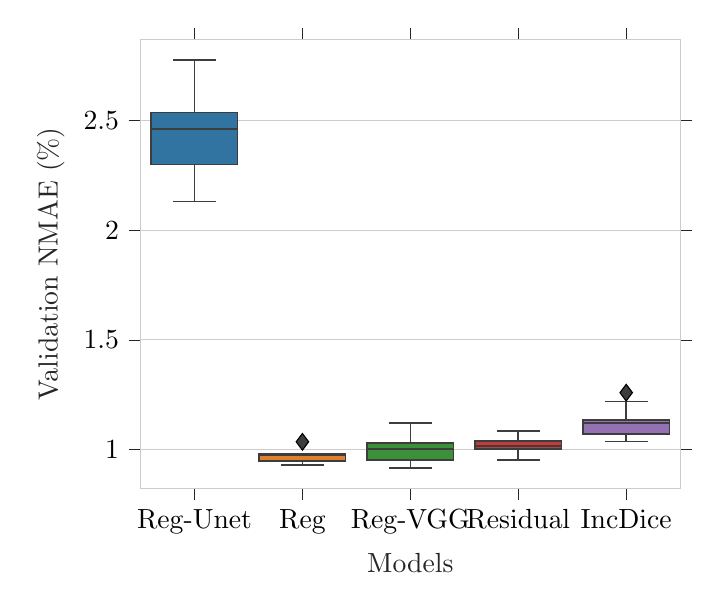
\begin{tikzpicture}

\definecolor{brown1926061}{RGB}{192,60,61}
\definecolor{darkslategray38}{RGB}{38,38,38}
\definecolor{darkslategray61}{RGB}{61,61,61}
\definecolor{lightgray204}{RGB}{204,204,204}
\definecolor{mediumpurple147113178}{RGB}{147,113,178}
\definecolor{peru22412844}{RGB}{224,128,44}
\definecolor{seagreen5814558}{RGB}{58,145,58}
\definecolor{steelblue49115161}{RGB}{49,115,161}

\begin{axis}[
axis line style={lightgray204},
tick align=outside,
x grid style={lightgray204},
xlabel=\textcolor{darkslategray38}{Models},
%xmajorticks=false,
xmin=-0.5, xmax=4.5,
xtick style={color=darkslategray38},
xtick={0,1,2,3,4},
xticklabels={Reg-Unet,Reg,Reg-VGG,Residual,IncDice},
y grid style={lightgray204},
ylabel=\textcolor{darkslategray38}{Validation NMAE (\%)},
ymajorgrids,
%ymajorticks=false,
ymin=0.824078426620843, ymax=2.86754917854291,
ytick style={color=darkslategray38}
]
\path [draw=darkslategray61, fill=steelblue49115161, semithick]
(axis cs:-0.4,2.2984584545917)
--(axis cs:0.4,2.2984584545917)
--(axis cs:0.4,2.53669090687491)
--(axis cs:-0.4,2.53669090687491)
--(axis cs:-0.4,2.2984584545917)
--cycle;
\path [draw=darkslategray61, fill=peru22412844, semithick]
(axis cs:0.6,0.947334674167854)
--(axis cs:1.4,0.947334674167854)
--(axis cs:1.4,0.980838016621642)
--(axis cs:0.6,0.980838016621642)
--(axis cs:0.6,0.947334674167854)
--cycle;
\path [draw=darkslategray61, fill=seagreen5814558, semithick]
(axis cs:1.6,0.953419044459612)
--(axis cs:2.4,0.953419044459612)
--(axis cs:2.4,1.02836175359939)
--(axis cs:1.6,1.02836175359939)
--(axis cs:1.6,0.953419044459612)
--cycle;
\path [draw=darkslategray61, fill=brown1926061, semithick]
(axis cs:2.6,1.00322149137223)
--(axis cs:3.4,1.00322149137223)
--(axis cs:3.4,1.03937849935059)
--(axis cs:2.6,1.03937849935059)
--(axis cs:2.6,1.00322149137223)
--cycle;
\path [draw=darkslategray61, fill=mediumpurple147113178, semithick]
(axis cs:3.6,1.07047335086434)
--(axis cs:4.4,1.07047335086434)
--(axis cs:4.4,1.13296523841858)
--(axis cs:3.6,1.13296523841858)
--(axis cs:3.6,1.07047335086434)
--cycle;
\addplot [semithick, darkslategray61]
table {%
0 2.2984584545917
0 2.1299203338543
};
\addplot [semithick, darkslategray61]
table {%
0 2.53669090687491
0 2.77466414436464
};
\addplot [semithick, darkslategray61]
table {%
-0.2 2.1299203338543
0.2 2.1299203338543
};
\addplot [semithick, darkslategray61]
table {%
-0.2 2.77466414436464
0.2 2.77466414436464
};
\addplot [semithick, darkslategray61]
table {%
1 0.947334674167854
1 0.929467934758842
};
\addplot [semithick, darkslategray61]
table {%
1 0.980838016621642
1 0.981920920492706
};
\addplot [semithick, darkslategray61]
table {%
0.8 0.929467934758842
1.2 0.929467934758842
};
\addplot [semithick, darkslategray61]
table {%
0.8 0.981920920492706
1.2 0.981920920492706
};
\addplot [black, mark=diamond*, mark size=3, mark options={solid,fill=darkslategray61}, only marks]
table {%
1 1.03497945645865
};
\addplot [semithick, darkslategray61]
table {%
2 0.953419044459612
2 0.916963460799119
};
\addplot [semithick, darkslategray61]
table {%
2 1.02836175359939
2 1.12179146130924
};
\addplot [semithick, darkslategray61]
table {%
1.8 0.916963460799119
2.2 0.916963460799119
};
\addplot [semithick, darkslategray61]
table {%
1.8 1.12179146130924
2.2 1.12179146130924
};
\addplot [semithick, darkslategray61]
table {%
3 1.00322149137223
3 0.953127496671489
};
\addplot [semithick, darkslategray61]
table {%
3 1.03937849935059
3 1.08444552072626
};
\addplot [semithick, darkslategray61]
table {%
2.8 0.953127496671489
3.2 0.953127496671489
};
\addplot [semithick, darkslategray61]
table {%
2.8 1.08444552072626
3.2 1.08444552072626
};
\addplot [semithick, darkslategray61]
table {%
4 1.07047335086434
4 1.03664159163596
};
\addplot [semithick, darkslategray61]
table {%
4 1.13296523841858
4 1.2191520301375
};
\addplot [semithick, darkslategray61]
table {%
3.8 1.03664159163596
4.2 1.03664159163596
};
\addplot [semithick, darkslategray61]
table {%
3.8 1.2191520301375
4.2 1.2191520301375
};
\addplot [black, mark=diamond*, mark size=3, mark options={solid,fill=darkslategray61}, only marks]
table {%
4 1.25900291720206
};
\addplot [semithick, darkslategray61]
table {%
-0.4 2.46143520423071
0.4 2.46143520423071
};
\addplot [semithick, darkslategray61]
table {%
0.6 0.97304395178237
1.4 0.97304395178237
};
\addplot [semithick, darkslategray61]
table {%
1.6 1.00145276360633
2.4 1.00145276360633
};
\addplot [semithick, darkslategray61]
table {%
2.6 1.01684802096654
3.4 1.01684802096654
};
\addplot [semithick, darkslategray61]
table {%
3.6 1.11961276712113
4.4 1.11961276712113
};
\end{axis}

\end{tikzpicture}

\caption{Box diagram of validation loss, i.e., the average NMAE (\%) of the density estimations for the validation set, for the 10 trainings and the 4 regression models considered plus the Inc-Dice segmentation DL. Outliers are represented with diamonds.}  
\label{fig:ValReg}
\end{figure}

%\begin{figure}[htbp]
%\centering
%\begin{tabular}{cccc}
% \includegraphics[width=8.3cm]{../figsDef/Val_Error_Reg_Imp.png}
%\end{tabular}
%\caption{Box diagram of percentage error in the density estimations for the validation set when using the three regression models desgined and the improvements are incorpored.} \label{fig:Error_Reg_Imp}
%\end{figure}



In view of the validation NMAE values in Fig. \ref{fig:ValReg} it can be concluded that the Reg-Unet approach is not a good option, i.e., reusing the encoder of the segmentation is not useful. On the contrary, the Reg, Reg-VGG, and Reg-Res approaches provide good low values with low variation of the results for the 10 trainings. The Inc-Dice model in \cite{Bejarano2023} with lowest NMAE achieved 1.12\% while with the improvements in Section \ref{sec:DG} we have a NMAE of 1.04\%, i.e., we have a 0.8\% improvement. The Inc-Dice model, however, presents an important increase when evaluated with test data, see Fig. \ref{fig:TestError}. 

Among the evaluated methods the Reg-VGG exhibits the lowest value of NMAE for the validation set, 0.92\%. We will use this model in the analysis of the canvases later in this work. Hence, compared to the segmentation DL approach the regression DL method has a 0.12\% lower error and does not need further signal processing as it directly computes the thread densities. 

When evaluated in the test set, see Fig. \ref{fig:TestError},  regression DL models have a very much better error value than the Inc-Dice.  Specifically, the NMAE in test has decreased from 1.51\% of the Inc-Dice to 1.02\% of the Reg-VGG for the best model in validation. The NMAE of the Inc-Dice as in \cite{Bejarano2023}, i.e., without the improvements in the generation of the dataset, increases to 1.61\%. %
%En el código de aquí está en 2.08\%. Se ha tomado el valor del paper de segmentación para q=0., ver q, porque si no sería 1.61\%.
 
\begin{figure}[htbp]
\centering
% This file was created with tikzplotlib v0.10.1.
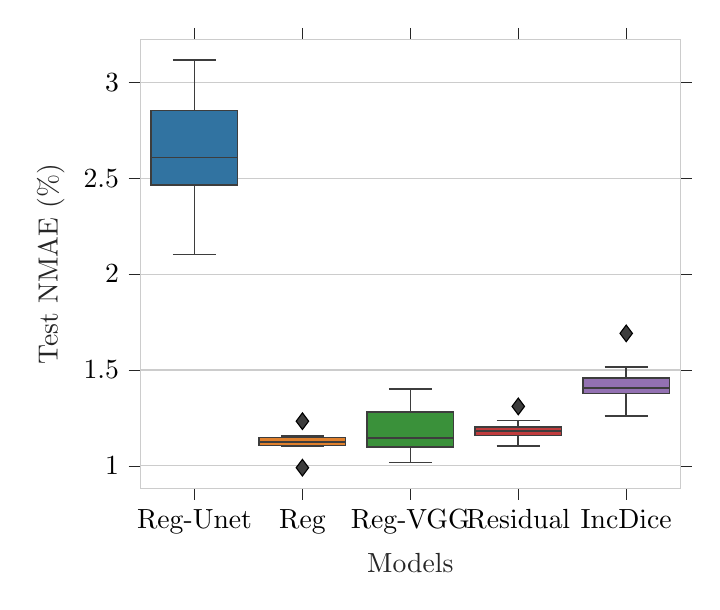
\begin{tikzpicture}

\definecolor{brown1926061}{RGB}{192,60,61}
\definecolor{darkslategray38}{RGB}{38,38,38}
\definecolor{darkslategray61}{RGB}{61,61,61}
\definecolor{lightgray204}{RGB}{204,204,204}
\definecolor{mediumpurple147113178}{RGB}{147,113,178}
\definecolor{peru22412844}{RGB}{224,128,44}
\definecolor{seagreen5814558}{RGB}{58,145,58}
\definecolor{steelblue49115161}{RGB}{49,115,161}

\begin{axis}[
axis line style={lightgray204},
tick align=outside,
x grid style={lightgray204},
xlabel=\textcolor{darkslategray38}{Models},
%xmajorticks=false,
xmin=-0.5, xmax=4.5,
xtick style={color=darkslategray38},
xtick={0,1,2,3,4},
xticklabels={Reg-Unet,Reg,Reg-VGG,Residual,IncDice},
y grid style={lightgray204},
ylabel=\textcolor{darkslategray38}{Test NMAE (\%)},
ymajorgrids,
%ymajorticks=false,
ymin=0.884131081000669, ymax=3.22168287187362,
ytick style={color=darkslategray38}
]
\path [draw=darkslategray61, fill=steelblue49115161, semithick]
(axis cs:-0.4,2.46321942449928)
--(axis cs:0.4,2.46321942449928)
--(axis cs:0.4,2.85320356926887)
--(axis cs:-0.4,2.85320356926887)
--(axis cs:-0.4,2.46321942449928)
--cycle;
\path [draw=darkslategray61, fill=peru22412844, semithick]
(axis cs:0.6,1.10643239003629)
--(axis cs:1.4,1.10643239003629)
--(axis cs:1.4,1.14736930873591)
--(axis cs:0.6,1.14736930873591)
--(axis cs:0.6,1.10643239003629)
--cycle;
\path [draw=darkslategray61, fill=seagreen5814558, semithick]
(axis cs:1.6,1.09855208092833)
--(axis cs:2.4,1.09855208092833)
--(axis cs:2.4,1.28099441629875)
--(axis cs:1.6,1.28099441629875)
--(axis cs:1.6,1.09855208092833)
--cycle;
\path [draw=darkslategray61, fill=brown1926061, semithick]
(axis cs:2.6,1.15811176892021)
--(axis cs:3.4,1.15811176892021)
--(axis cs:3.4,1.20159203112214)
--(axis cs:2.6,1.20159203112214)
--(axis cs:2.6,1.15811176892021)
--cycle;
\path [draw=darkslategray61, fill=mediumpurple147113178, semithick]
(axis cs:3.6,1.37707843452498)
--(axis cs:4.4,1.37707843452498)
--(axis cs:4.4,1.45982205890896)
--(axis cs:3.6,1.45982205890896)
--(axis cs:3.6,1.37707843452498)
--cycle;
\addplot [semithick, darkslategray61]
table {%
0 2.46321942449928
0 2.10203285079398
};
\addplot [semithick, darkslategray61]
table {%
0 2.85320356926887
0 3.11543051774303
};
\addplot [semithick, darkslategray61]
table {%
-0.2 2.10203285079398
0.2 2.10203285079398
};
\addplot [semithick, darkslategray61]
table {%
-0.2 3.11543051774303
0.2 3.11543051774303
};
\addplot [semithick, darkslategray61]
table {%
1 1.10643239003629
1 1.10111523089775
};
\addplot [semithick, darkslategray61]
table {%
1 1.14736930873591
1 1.15455019371843
};
\addplot [semithick, darkslategray61]
table {%
0.8 1.10111523089775
1.2 1.10111523089775
};
\addplot [semithick, darkslategray61]
table {%
0.8 1.15455019371843
1.2 1.15455019371843
};
\addplot [black, mark=diamond*, mark size=3, mark options={solid,fill=darkslategray61}, only marks]
table {%
1 0.990383435131258
1 1.23289321681174
};
\addplot [semithick, darkslategray61]
table {%
2 1.09855208092833
2 1.01692288173621
};
\addplot [semithick, darkslategray61]
table {%
2 1.28099441629875
2 1.40016160616263
};
\addplot [semithick, darkslategray61]
table {%
1.8 1.01692288173621
2.2 1.01692288173621
};
\addplot [semithick, darkslategray61]
table {%
1.8 1.40016160616263
2.2 1.40016160616263
};
\addplot [semithick, darkslategray61]
table {%
3 1.15811176892021
3 1.10204894654453
};
\addplot [semithick, darkslategray61]
table {%
3 1.20159203112214
3 1.23630047399395
};
\addplot [semithick, darkslategray61]
table {%
2.8 1.10204894654453
3.2 1.10204894654453
};
\addplot [semithick, darkslategray61]
table {%
2.8 1.23630047399395
3.2 1.23630047399395
};
\addplot [black, mark=diamond*, mark size=3, mark options={solid,fill=darkslategray61}, only marks]
table {%
3 1.30994310375212
};
\addplot [semithick, darkslategray61]
table {%
4 1.37707843452498
4 1.26050060008103
};
\addplot [semithick, darkslategray61]
table {%
4 1.45982205890896
4 1.51452619650304
};
\addplot [semithick, darkslategray61]
table {%
3.8 1.26050060008103
4.2 1.26050060008103
};
\addplot [semithick, darkslategray61]
table {%
3.8 1.51452619650304
4.2 1.51452619650304
};
\addplot [black, mark=diamond*, mark size=3, mark options={solid,fill=darkslategray61}, only marks]
table {%
4 1.6908036979183
};
\addplot [semithick, darkslategray61]
table {%
-0.4 2.60785504194306
0.4 2.60785504194306
};
\addplot [semithick, darkslategray61]
table {%
0.6 1.12386538083148
1.4 1.12386538083148
};
\addplot [semithick, darkslategray61]
table {%
1.6 1.14365093431843
2.4 1.14365093431843
};
\addplot [semithick, darkslategray61]
table {%
2.6 1.1820777529085
3.4 1.1820777529085
};
\addplot [semithick, darkslategray61]
table {%
3.6 1.40433455532713
4.4 1.40433455532713
};
\end{axis}

\end{tikzpicture}

% \includegraphics[width=8cm]{../figsDef/boxRegressionTestNMAE.png}%Test_Error.png}
\caption{Box diagram of the average NMAE (\%) of the density estimations for the test set, for the 10 trainings and the 4 regression models considered and the Inc-Dice segmentation DL. Outliers are represented with diamonds.} \label{fig:TestError}
\end{figure}

%\begin{figure*}[htp]
%\centering
%\input{../figsDef/RegressionTest.tex}
%\caption{CAMBIARRRNormalized absolute error ($\%$) in horizontal (\textcolor{blue}{$\circ$} solid) and vertical (\textcolor{red}{$\diamond$} dashed) densities for the $1\times 1$ cm corners of the $1.5\times 1.5$ cm annotated crops in the test set and Inception VGG-Based Regression Model used.} \label{fig:errorRegTest}
%\end{figure*}
%
%
%
%\begin{figure*}[htp]
%\centering
%% This file was created with tikzplotlib v0.10.1.
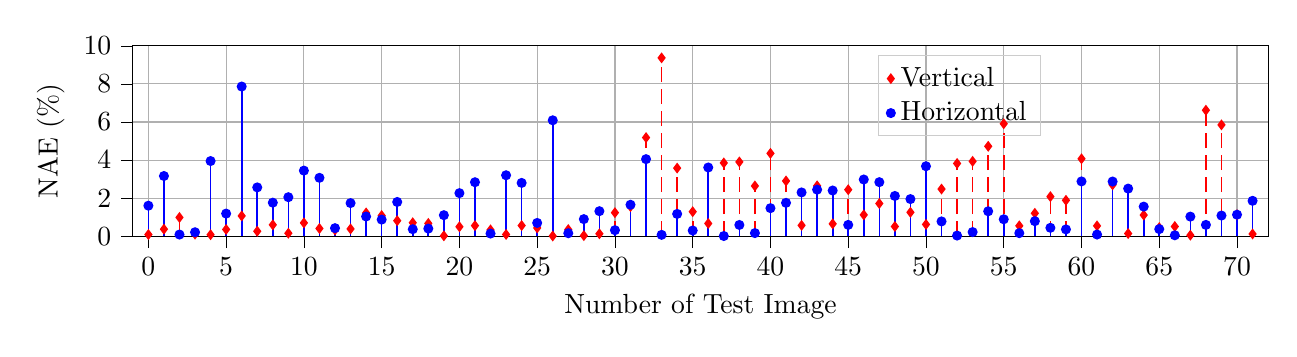
\begin{tikzpicture}

\definecolor{darkgray176}{RGB}{176,176,176}
\definecolor{lightgray204}{RGB}{204,204,204}

\begin{axis}[
width = 16cm,
height = 4cm,
legend cell align={left},
legend style={fill=none, text opacity=1, draw=lightgray204, at={(0.8,0.95)} },
tick align=outside,
tick pos=left,
x grid style={darkgray176},
xlabel={Number of Test Image},
xmajorgrids,
xmin=-1, xmax=72,
xtick style={color=black},
y grid style={darkgray176},
ylabel={NAE (\%)},
ymajorgrids,
ymin=0, ymax=10,
ytick style={color=black}
]
\path [draw=red, semithick, dash pattern=on 5.55pt off 2.4pt]
(axis cs:0,0)
--(axis cs:0,0.0891372893177833);

\path [draw=red, semithick, dash pattern=on 5.55pt off 2.4pt]
(axis cs:1,0)
--(axis cs:1,0.370584604455035);

\path [draw=red, semithick, dash pattern=on 5.55pt off 2.4pt]
(axis cs:2,0)
--(axis cs:2,0.986032709471848);

\path [draw=red, semithick, dash pattern=on 5.55pt off 2.4pt]
(axis cs:3,0)
--(axis cs:3,0.109907766079546);

\path [draw=red, semithick, dash pattern=on 5.55pt off 2.4pt]
(axis cs:4,0)
--(axis cs:4,0.0822666596545819);

\path [draw=red, semithick, dash pattern=on 5.55pt off 2.4pt]
(axis cs:5,0)
--(axis cs:5,0.357321088428495);

\path [draw=red, semithick, dash pattern=on 5.55pt off 2.4pt]
(axis cs:6,0)
--(axis cs:6,1.0675179989252);

\path [draw=red, semithick, dash pattern=on 5.55pt off 2.4pt]
(axis cs:7,0)
--(axis cs:7,0.26087508855736);

\path [draw=red, semithick, dash pattern=on 5.55pt off 2.4pt]
(axis cs:8,0)
--(axis cs:8,0.599942897007989);

\path [draw=red, semithick, dash pattern=on 5.55pt off 2.4pt]
(axis cs:9,0)
--(axis cs:9,0.157795275627521);

\path [draw=red, semithick, dash pattern=on 5.55pt off 2.4pt]
(axis cs:10,0)
--(axis cs:10,0.702147162506958);

\path [draw=red, semithick, dash pattern=on 5.55pt off 2.4pt]
(axis cs:11,0)
--(axis cs:11,0.406909215796071);

\path [draw=red, semithick, dash pattern=on 5.55pt off 2.4pt]
(axis cs:12,0)
--(axis cs:12,0.331458806193995);

\path [draw=red, semithick, dash pattern=on 5.55pt off 2.4pt]
(axis cs:13,0)
--(axis cs:13,0.383915047035242);

\path [draw=red, semithick, dash pattern=on 5.55pt off 2.4pt]
(axis cs:14,0)
--(axis cs:14,1.22389293172749);

\path [draw=red, semithick, dash pattern=on 5.55pt off 2.4pt]
(axis cs:15,0)
--(axis cs:15,1.08618673878954);

\path [draw=red, semithick, dash pattern=on 5.55pt off 2.4pt]
(axis cs:16,0)
--(axis cs:16,0.817461271972514);

\path [draw=red, semithick, dash pattern=on 5.55pt off 2.4pt]
(axis cs:17,0)
--(axis cs:17,0.708983367636591);

\path [draw=red, semithick, dash pattern=on 5.55pt off 2.4pt]
(axis cs:18,0)
--(axis cs:18,0.674357282147208);

\path [draw=red, semithick, dash pattern=on 5.55pt off 2.4pt]
(axis cs:19,0)
--(axis cs:19,0.0228714579279005);

\path [draw=red, semithick, dash pattern=on 5.55pt off 2.4pt]
(axis cs:20,0)
--(axis cs:20,0.497540760406243);

\path [draw=red, semithick, dash pattern=on 5.55pt off 2.4pt]
(axis cs:21,0)
--(axis cs:21,0.557443349354307);

\path [draw=red, semithick, dash pattern=on 5.55pt off 2.4pt]
(axis cs:22,0)
--(axis cs:22,0.33349683417564);

\path [draw=red, semithick, dash pattern=on 5.55pt off 2.4pt]
(axis cs:23,0)
--(axis cs:23,0.0933148019058486);

\path [draw=red, semithick, dash pattern=on 5.55pt off 2.4pt]
(axis cs:24,0)
--(axis cs:24,0.561745742877895);

\path [draw=red, semithick, dash pattern=on 5.55pt off 2.4pt]
(axis cs:25,0)
--(axis cs:25,0.435179364185227);

\path [draw=red, semithick, dash pattern=on 5.55pt off 2.4pt]
(axis cs:26,0)
--(axis cs:26,0.0115060568569611);

\path [draw=red, semithick, dash pattern=on 5.55pt off 2.4pt]
(axis cs:27,0)
--(axis cs:27,0.353191168275281);

\path [draw=red, semithick, dash pattern=on 5.55pt off 2.4pt]
(axis cs:28,0)
--(axis cs:28,0.03307448084071);

\path [draw=red, semithick, dash pattern=on 5.55pt off 2.4pt]
(axis cs:29,0)
--(axis cs:29,0.128556121680998);

\path [draw=red, semithick, dash pattern=on 5.55pt off 2.4pt]
(axis cs:30,0)
--(axis cs:30,1.23797858204359);

\path [draw=red, semithick, dash pattern=on 5.55pt off 2.4pt]
(axis cs:31,0)
--(axis cs:31,1.55669577142518);

\path [draw=red, semithick, dash pattern=on 5.55pt off 2.4pt]
(axis cs:32,0)
--(axis cs:32,5.18087173679666);

\path [draw=red, semithick, dash pattern=on 5.55pt off 2.4pt]
(axis cs:33,0)
--(axis cs:33,9.36596359845506);

\path [draw=red, semithick, dash pattern=on 5.55pt off 2.4pt]
(axis cs:34,0)
--(axis cs:34,3.57877826385229);

\path [draw=red, semithick, dash pattern=on 5.55pt off 2.4pt]
(axis cs:35,0)
--(axis cs:35,1.28796097434612);

\path [draw=red, semithick, dash pattern=on 5.55pt off 2.4pt]
(axis cs:36,0)
--(axis cs:36,0.670376647450484);

\path [draw=red, semithick, dash pattern=on 5.55pt off 2.4pt]
(axis cs:37,0)
--(axis cs:37,3.849417073192);

\path [draw=red, semithick, dash pattern=on 5.55pt off 2.4pt]
(axis cs:38,0)
--(axis cs:38,3.90441689015446);

\path [draw=red, semithick, dash pattern=on 5.55pt off 2.4pt]
(axis cs:39,0)
--(axis cs:39,2.64135164715969);

\path [draw=red, semithick, dash pattern=on 5.55pt off 2.4pt]
(axis cs:40,0)
--(axis cs:40,4.35127206115533);

\path [draw=red, semithick, dash pattern=on 5.55pt off 2.4pt]
(axis cs:41,0)
--(axis cs:41,2.90353625220088);

\path [draw=red, semithick, dash pattern=on 5.55pt off 2.4pt]
(axis cs:42,0)
--(axis cs:42,0.57060967755702);

\path [draw=red, semithick, dash pattern=on 5.55pt off 2.4pt]
(axis cs:43,0)
--(axis cs:43,2.64672702718658);

\path [draw=red, semithick, dash pattern=on 5.55pt off 2.4pt]
(axis cs:44,0)
--(axis cs:44,0.652177730307519);

\path [draw=red, semithick, dash pattern=on 5.55pt off 2.4pt]
(axis cs:45,0)
--(axis cs:45,2.44257111815915);

\path [draw=red, semithick, dash pattern=on 5.55pt off 2.4pt]
(axis cs:46,0)
--(axis cs:46,1.1222012979615);

\path [draw=red, semithick, dash pattern=on 5.55pt off 2.4pt]
(axis cs:47,0)
--(axis cs:47,1.7182354098259);

\path [draw=red, semithick, dash pattern=on 5.55pt off 2.4pt]
(axis cs:48,0)
--(axis cs:48,0.510461785691346);

\path [draw=red, semithick, dash pattern=on 5.55pt off 2.4pt]
(axis cs:49,0)
--(axis cs:49,1.25633791423234);

\path [draw=red, semithick, dash pattern=on 5.55pt off 2.4pt]
(axis cs:50,0)
--(axis cs:50,0.621333507441592);

\path [draw=red, semithick, dash pattern=on 5.55pt off 2.4pt]
(axis cs:51,0)
--(axis cs:51,2.47832255794163);

\path [draw=red, semithick, dash pattern=on 5.55pt off 2.4pt]
(axis cs:52,0)
--(axis cs:52,3.82364348447404);

\path [draw=red, semithick, dash pattern=on 5.55pt off 2.4pt]
(axis cs:53,0)
--(axis cs:53,3.93376682815643);

\path [draw=red, semithick, dash pattern=on 5.55pt off 2.4pt]
(axis cs:54,0)
--(axis cs:54,4.72364348422319);

\path [draw=red, semithick, dash pattern=on 5.55pt off 2.4pt]
(axis cs:55,0)
--(axis cs:55,5.90572014967425);

\path [draw=red, semithick, dash pattern=on 5.55pt off 2.4pt]
(axis cs:56,0)
--(axis cs:56,0.545846235128202);

\path [draw=red, semithick, dash pattern=on 5.55pt off 2.4pt]
(axis cs:57,0)
--(axis cs:57,1.20550889099103);

\path [draw=red, semithick, dash pattern=on 5.55pt off 2.4pt]
(axis cs:58,0)
--(axis cs:58,2.0798141224854);

\path [draw=red, semithick, dash pattern=on 5.55pt off 2.4pt]
(axis cs:59,0)
--(axis cs:59,1.88769559832437);

\path [draw=red, semithick, dash pattern=on 5.55pt off 2.4pt]
(axis cs:60,0)
--(axis cs:60,4.06760766382771);

\path [draw=red, semithick, dash pattern=on 5.55pt off 2.4pt]
(axis cs:61,0)
--(axis cs:61,0.544880396955417);

\path [draw=red, semithick, dash pattern=on 5.55pt off 2.4pt]
(axis cs:62,0)
--(axis cs:62,2.70220218089618);

\path [draw=red, semithick, dash pattern=on 5.55pt off 2.4pt]
(axis cs:63,0)
--(axis cs:63,0.142450855369382);

\path [draw=red, semithick, dash pattern=on 5.55pt off 2.4pt]
(axis cs:64,0)
--(axis cs:64,1.11221061384018);

\path [draw=red, semithick, dash pattern=on 5.55pt off 2.4pt]
(axis cs:65,0)
--(axis cs:65,0.455836859781922);

\path [draw=red, semithick, dash pattern=on 5.55pt off 2.4pt]
(axis cs:66,0)
--(axis cs:66,0.512493203062239);

\path [draw=red, semithick, dash pattern=on 5.55pt off 2.4pt]
(axis cs:67,0)
--(axis cs:67,0.0541307805128674);

\path [draw=red, semithick, dash pattern=on 5.55pt off 2.4pt]
(axis cs:68,0)
--(axis cs:68,6.61802465938199);

\path [draw=red, semithick, dash pattern=on 5.55pt off 2.4pt]
(axis cs:69,0)
--(axis cs:69,5.84877015002152);

\path [draw=red, semithick, dash pattern=on 5.55pt off 2.4pt]
(axis cs:70,0)
--(axis cs:70,1.13183003764784);

\path [draw=red, semithick, dash pattern=on 5.55pt off 2.4pt]
(axis cs:71,0)
--(axis cs:71,0.120663657892921);

\path [draw=blue, semithick]
(axis cs:0,0)
--(axis cs:0,1.60482432359047);

\path [draw=blue, semithick]
(axis cs:1,0)
--(axis cs:1,3.16337308379479);

\path [draw=blue, semithick]
(axis cs:2,0)
--(axis cs:2,0.088518954929298);

\path [draw=blue, semithick]
(axis cs:3,0)
--(axis cs:3,0.209946522328121);

\path [draw=blue, semithick]
(axis cs:4,0)
--(axis cs:4,3.94868101726816);

\path [draw=blue, semithick]
(axis cs:5,0)
--(axis cs:5,1.1890567311829);

\path [draw=blue, semithick]
(axis cs:6,0)
--(axis cs:6,7.86157482848479);

\path [draw=blue, semithick]
(axis cs:7,0)
--(axis cs:7,2.56533097803157);

\path [draw=blue, semithick]
(axis cs:8,0)
--(axis cs:8,1.76323691381998);

\path [draw=blue, semithick]
(axis cs:9,0)
--(axis cs:9,2.05101657514193);

\path [draw=blue, semithick]
(axis cs:10,0)
--(axis cs:10,3.44695063169501);

\path [draw=blue, semithick]
(axis cs:11,0)
--(axis cs:11,3.06769932233839);

\path [draw=blue, semithick]
(axis cs:12,0)
--(axis cs:12,0.425124444156019);

\path [draw=blue, semithick]
(axis cs:13,0)
--(axis cs:13,1.74108652685822);

\path [draw=blue, semithick]
(axis cs:14,0)
--(axis cs:14,1.03592652805637);

\path [draw=blue, semithick]
(axis cs:15,0)
--(axis cs:15,0.874851553696532);

\path [draw=blue, semithick]
(axis cs:16,0)
--(axis cs:16,1.80032370895501);

\path [draw=blue, semithick]
(axis cs:17,0)
--(axis cs:17,0.369830616734339);

\path [draw=blue, semithick]
(axis cs:18,0)
--(axis cs:18,0.401111073332179);

\path [draw=blue, semithick]
(axis cs:19,0)
--(axis cs:19,1.10642535423046);

\path [draw=blue, semithick]
(axis cs:20,0)
--(axis cs:20,2.26387154762841);

\path [draw=blue, semithick]
(axis cs:21,0)
--(axis cs:21,2.83718646720633);

\path [draw=blue, semithick]
(axis cs:22,0)
--(axis cs:22,0.1406937077281);

\path [draw=blue, semithick]
(axis cs:23,0)
--(axis cs:23,3.20267812839011);

\path [draw=blue, semithick]
(axis cs:24,0)
--(axis cs:24,2.80031096883609);

\path [draw=blue, semithick]
(axis cs:25,0)
--(axis cs:25,0.699085408205588);

\path [draw=blue, semithick]
(axis cs:26,0)
--(axis cs:26,6.08843810697338);

\path [draw=blue, semithick]
(axis cs:27,0)
--(axis cs:27,0.15864254759884);

\path [draw=blue, semithick]
(axis cs:28,0)
--(axis cs:28,0.89939964672912);

\path [draw=blue, semithick]
(axis cs:29,0)
--(axis cs:29,1.31660840779235);

\path [draw=blue, semithick]
(axis cs:30,0)
--(axis cs:30,0.318010242119301);

\path [draw=blue, semithick]
(axis cs:31,0)
--(axis cs:31,1.65439344125001);

\path [draw=blue, semithick]
(axis cs:32,0)
--(axis cs:32,4.0483540218392);

\path [draw=blue, semithick]
(axis cs:33,0)
--(axis cs:33,0.0730891529074287);

\path [draw=blue, semithick]
(axis cs:34,0)
--(axis cs:34,1.17231958118489);

\path [draw=blue, semithick]
(axis cs:35,0)
--(axis cs:35,0.300970256518251);

\path [draw=blue, semithick]
(axis cs:36,0)
--(axis cs:36,3.61055197209082);

\path [draw=blue, semithick]
(axis cs:37,0)
--(axis cs:37,0.012149964675335);

\path [draw=blue, semithick]
(axis cs:38,0)
--(axis cs:38,0.592998250688215);

\path [draw=blue, semithick]
(axis cs:39,0)
--(axis cs:39,0.164741687083903);

\path [draw=blue, semithick]
(axis cs:40,0)
--(axis cs:40,1.47468837822852);

\path [draw=blue, semithick]
(axis cs:41,0)
--(axis cs:41,1.75416009928301);

\path [draw=blue, semithick]
(axis cs:42,0)
--(axis cs:42,2.30136441803097);

\path [draw=blue, semithick]
(axis cs:43,0)
--(axis cs:43,2.44754392202821);

\path [draw=blue, semithick]
(axis cs:44,0)
--(axis cs:44,2.40126263823437);

\path [draw=blue, semithick]
(axis cs:45,0)
--(axis cs:45,0.596231763375445);

\path [draw=blue, semithick]
(axis cs:46,0)
--(axis cs:46,2.97974726299161);

\path [draw=blue, semithick]
(axis cs:47,0)
--(axis cs:47,2.8403540068345);

\path [draw=blue, semithick]
(axis cs:48,0)
--(axis cs:48,2.11609785007945);

\path [draw=blue, semithick]
(axis cs:49,0)
--(axis cs:49,1.95178155012636);

\path [draw=blue, semithick]
(axis cs:50,0)
--(axis cs:50,3.67679795630587);

\path [draw=blue, semithick]
(axis cs:51,0)
--(axis cs:51,0.778316601196557);

\path [draw=blue, semithick]
(axis cs:52,0)
--(axis cs:52,0.0354201830380699);

\path [draw=blue, semithick]
(axis cs:53,0)
--(axis cs:53,0.219323231101386);

\path [draw=blue, semithick]
(axis cs:54,0)
--(axis cs:54,1.31106498447003);

\path [draw=blue, semithick]
(axis cs:55,0)
--(axis cs:55,0.891170629365694);

\path [draw=blue, semithick]
(axis cs:56,0)
--(axis cs:56,0.162700341116095);

\path [draw=blue, semithick]
(axis cs:57,0)
--(axis cs:57,0.791304910412589);

\path [draw=blue, semithick]
(axis cs:58,0)
--(axis cs:58,0.442745412109532);

\path [draw=blue, semithick]
(axis cs:59,0)
--(axis cs:59,0.359649677668585);

\path [draw=blue, semithick]
(axis cs:60,0)
--(axis cs:60,2.87901485242971);

\path [draw=blue, semithick]
(axis cs:61,0)
--(axis cs:61,0.0890789423451848);

\path [draw=blue, semithick]
(axis cs:62,0)
--(axis cs:62,2.87360305730203);

\path [draw=blue, semithick]
(axis cs:63,0)
--(axis cs:63,2.50185328732075);

\path [draw=blue, semithick]
(axis cs:64,0)
--(axis cs:64,1.55591787676345);

\path [draw=blue, semithick]
(axis cs:65,0)
--(axis cs:65,0.373843770605919);

\path [draw=blue, semithick]
(axis cs:66,0)
--(axis cs:66,0.0500395673834782);

\path [draw=blue, semithick]
(axis cs:67,0)
--(axis cs:67,1.03094775175834);

\path [draw=blue, semithick]
(axis cs:68,0)
--(axis cs:68,0.596176262631349);

\path [draw=blue, semithick]
(axis cs:69,0)
--(axis cs:69,1.08649993637958);

\path [draw=blue, semithick]
(axis cs:70,0)
--(axis cs:70,1.13183586227048);

\path [draw=blue, semithick]
(axis cs:71,0)
--(axis cs:71,1.86047529565208);

\addplot [semithick, red, mark=diamond*, mark size=1.5, mark options={solid}, only marks]
table {%
0 0.0891372893177833
1 0.370584604455035
2 0.986032709471848
3 0.109907766079546
4 0.0822666596545819
5 0.357321088428495
6 1.0675179989252
7 0.26087508855736
8 0.599942897007989
9 0.157795275627521
10 0.702147162506958
11 0.406909215796071
12 0.331458806193995
13 0.383915047035242
14 1.22389293172749
15 1.08618673878954
16 0.817461271972514
17 0.708983367636591
18 0.674357282147208
19 0.0228714579279005
20 0.497540760406243
21 0.557443349354307
22 0.33349683417564
23 0.0933148019058486
24 0.561745742877895
25 0.435179364185227
26 0.0115060568569611
27 0.353191168275281
28 0.03307448084071
29 0.128556121680998
30 1.23797858204359
31 1.55669577142518
32 5.18087173679666
33 9.36596359845506
34 3.57877826385229
35 1.28796097434612
36 0.670376647450484
37 3.849417073192
38 3.90441689015446
39 2.64135164715969
40 4.35127206115533
41 2.90353625220088
42 0.57060967755702
43 2.64672702718658
44 0.652177730307519
45 2.44257111815915
46 1.1222012979615
47 1.7182354098259
48 0.510461785691346
49 1.25633791423234
50 0.621333507441592
51 2.47832255794163
52 3.82364348447404
53 3.93376682815643
54 4.72364348422319
55 5.90572014967425
56 0.545846235128202
57 1.20550889099103
58 2.0798141224854
59 1.88769559832437
60 4.06760766382771
61 0.544880396955417
62 2.70220218089618
63 0.142450855369382
64 1.11221061384018
65 0.455836859781922
66 0.512493203062239
67 0.0541307805128674
68 6.61802465938199
69 5.84877015002152
70 1.13183003764784
71 0.120663657892921
};\addlegendentry{Vertical}
\addplot [semithick, blue, mark=*, mark size=1.5, mark options={solid}, only marks]
table {%
0 1.60482432359047
1 3.16337308379479
2 0.088518954929298
3 0.209946522328121
4 3.94868101726816
5 1.1890567311829
6 7.86157482848479
7 2.56533097803157
8 1.76323691381998
9 2.05101657514193
10 3.44695063169501
11 3.06769932233839
12 0.425124444156019
13 1.74108652685822
14 1.03592652805637
15 0.874851553696532
16 1.80032370895501
17 0.369830616734339
18 0.401111073332179
19 1.10642535423046
20 2.26387154762841
21 2.83718646720633
22 0.1406937077281
23 3.20267812839011
24 2.80031096883609
25 0.699085408205588
26 6.08843810697338
27 0.15864254759884
28 0.89939964672912
29 1.31660840779235
30 0.318010242119301
31 1.65439344125001
32 4.0483540218392
33 0.0730891529074287
34 1.17231958118489
35 0.300970256518251
36 3.61055197209082
37 0.012149964675335
38 0.592998250688215
39 0.164741687083903
40 1.47468837822852
41 1.75416009928301
42 2.30136441803097
43 2.44754392202821
44 2.40126263823437
45 0.596231763375445
46 2.97974726299161
47 2.8403540068345
48 2.11609785007945
49 1.95178155012636
50 3.67679795630587
51 0.778316601196557
52 0.0354201830380699
53 0.219323231101386
54 1.31106498447003
55 0.891170629365694
56 0.162700341116095
57 0.791304910412589
58 0.442745412109532
59 0.359649677668585
60 2.87901485242971
61 0.0890789423451848
62 2.87360305730203
63 2.50185328732075
64 1.55591787676345
65 0.373843770605919
66 0.0500395673834782
67 1.03094775175834
68 0.596176262631349
69 1.08649993637958
70 1.13183586227048
71 1.86047529565208
};\addlegendentry{Horizontal}
\end{axis}

\end{tikzpicture}

%\caption{Normalized absolute error ($\%$) in horizontal (\textcolor{blue}{$\circ$} solid) and vertical (\textcolor{red}{$\diamond$} dashed) densities  for the $1\times 1$ cm corners of the $1.5\times 1.5$ cm annotated crops in the test set and the segmentation plus image-processing algorithms used. } \label{fig:AA}
%\end{figure*}
%
%\begin{figure*}[htp]
%\centering
%% This file was created with tikzplotlib v0.10.1.
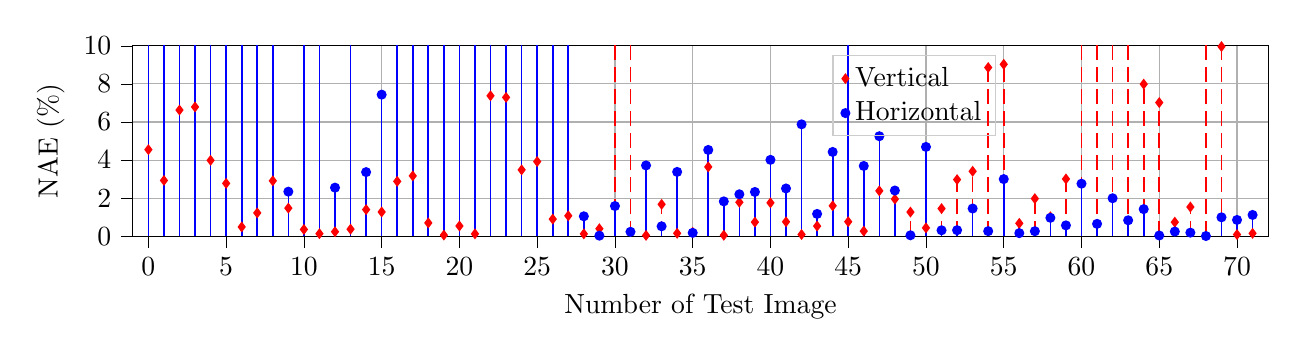
\begin{tikzpicture}

\definecolor{darkgray176}{RGB}{176,176,176}
\definecolor{lightgray204}{RGB}{204,204,204}

\begin{axis}[
width = 16cm,
height = 4cm,
legend cell align={left},
legend style={fill = none, text opacity=1, draw=lightgray204, at={(0.76,0.95)} },
tick align=outside,
tick pos=left,
x grid style={darkgray176},
xlabel={Number of Test Image},
xmajorgrids,
xmin=-1, xmax=72,
xtick style={color=black},
y grid style={darkgray176},
ylabel={NAE (\%)},
ymajorgrids,
ymin=0, ymax=10,
ytick style={color=black}
]
\path [draw=red, semithick, dash pattern=on 5.55pt off 2.4pt]
(axis cs:0,0)
--(axis cs:0,4.5483855778803);

\path [draw=red, semithick, dash pattern=on 5.55pt off 2.4pt]
(axis cs:1,0)
--(axis cs:1,2.9292841952533);

\path [draw=red, semithick, dash pattern=on 5.55pt off 2.4pt]
(axis cs:2,0)
--(axis cs:2,6.62645610841829);

\path [draw=red, semithick, dash pattern=on 5.55pt off 2.4pt]
(axis cs:3,0)
--(axis cs:3,6.78846952332171);

\path [draw=red, semithick, dash pattern=on 5.55pt off 2.4pt]
(axis cs:4,0)
--(axis cs:4,3.98599574299314);

\path [draw=red, semithick, dash pattern=on 5.55pt off 2.4pt]
(axis cs:5,0)
--(axis cs:5,2.7756684893379);

\path [draw=red, semithick, dash pattern=on 5.55pt off 2.4pt]
(axis cs:6,0)
--(axis cs:6,0.488267940090136);

\path [draw=red, semithick, dash pattern=on 5.55pt off 2.4pt]
(axis cs:7,0)
--(axis cs:7,1.22326551734608);

\path [draw=red, semithick, dash pattern=on 5.55pt off 2.4pt]
(axis cs:8,0)
--(axis cs:8,2.90977868853943);

\path [draw=red, semithick, dash pattern=on 5.55pt off 2.4pt]
(axis cs:9,0)
--(axis cs:9,1.47605435428485);

\path [draw=red, semithick, dash pattern=on 5.55pt off 2.4pt]
(axis cs:10,0)
--(axis cs:10,0.354545808613438);

\path [draw=red, semithick, dash pattern=on 5.55pt off 2.4pt]
(axis cs:11,0)
--(axis cs:11,0.134605226059808);

\path [draw=red, semithick, dash pattern=on 5.55pt off 2.4pt]
(axis cs:12,0)
--(axis cs:12,0.237049598001875);

\path [draw=red, semithick, dash pattern=on 5.55pt off 2.4pt]
(axis cs:13,0)
--(axis cs:13,0.37250971966461);

\path [draw=red, semithick, dash pattern=on 5.55pt off 2.4pt]
(axis cs:14,0)
--(axis cs:14,1.40024444895354);

\path [draw=red, semithick, dash pattern=on 5.55pt off 2.4pt]
(axis cs:15,0)
--(axis cs:15,1.27429629808493);

\path [draw=red, semithick, dash pattern=on 5.55pt off 2.4pt]
(axis cs:16,0)
--(axis cs:16,2.88289168100941);

\path [draw=red, semithick, dash pattern=on 5.55pt off 2.4pt]
(axis cs:17,0)
--(axis cs:17,3.1686077537258);

\path [draw=red, semithick, dash pattern=on 5.55pt off 2.4pt]
(axis cs:18,0)
--(axis cs:18,0.699726065157247);

\path [draw=red, semithick, dash pattern=on 5.55pt off 2.4pt]
(axis cs:19,0)
--(axis cs:19,0.0589048045037918);

\path [draw=red, semithick, dash pattern=on 5.55pt off 2.4pt]
(axis cs:20,0)
--(axis cs:20,0.538795448616386);

\path [draw=red, semithick, dash pattern=on 5.55pt off 2.4pt]
(axis cs:21,0)
--(axis cs:21,0.123797425539182);

\path [draw=red, semithick, dash pattern=on 5.55pt off 2.4pt]
(axis cs:22,0)
--(axis cs:22,7.37726584973173);

\path [draw=red, semithick, dash pattern=on 5.55pt off 2.4pt]
(axis cs:23,0)
--(axis cs:23,7.29103705633353);

\path [draw=red, semithick, dash pattern=on 5.55pt off 2.4pt]
(axis cs:24,0)
--(axis cs:24,3.48592496172199);

\path [draw=red, semithick, dash pattern=on 5.55pt off 2.4pt]
(axis cs:25,0)
--(axis cs:25,3.92071541688619);

\path [draw=red, semithick, dash pattern=on 5.55pt off 2.4pt]
(axis cs:26,0)
--(axis cs:26,0.901441044251731);

\path [draw=red, semithick, dash pattern=on 5.55pt off 2.4pt]
(axis cs:27,0)
--(axis cs:27,1.07347984999687);

\path [draw=red, semithick, dash pattern=on 5.55pt off 2.4pt]
(axis cs:28,0)
--(axis cs:28,0.125353601553148);

\path [draw=red, semithick, dash pattern=on 5.55pt off 2.4pt]
(axis cs:29,0)
--(axis cs:29,0.393938547036884);

\path [draw=red, semithick, dash pattern=on 5.55pt off 2.4pt]
(axis cs:30,0)
--(axis cs:30,16.3856469028772);

\path [draw=red, semithick, dash pattern=on 5.55pt off 2.4pt]
(axis cs:31,0)
--(axis cs:31,15.7549969136119);

\path [draw=red, semithick, dash pattern=on 5.55pt off 2.4pt]
(axis cs:32,0)
--(axis cs:32,0.0449959270112771);

\path [draw=red, semithick, dash pattern=on 5.55pt off 2.4pt]
(axis cs:33,0)
--(axis cs:33,1.67536462034163);

\path [draw=red, semithick, dash pattern=on 5.55pt off 2.4pt]
(axis cs:34,0)
--(axis cs:34,0.155591449976825);

\path [draw=red, semithick, dash pattern=on 5.55pt off 2.4pt]
(axis cs:35,0)
--(axis cs:35,0.20494097953652);

\path [draw=red, semithick, dash pattern=on 5.55pt off 2.4pt]
(axis cs:36,0)
--(axis cs:36,3.64091876176312);

\path [draw=red, semithick, dash pattern=on 5.55pt off 2.4pt]
(axis cs:37,0)
--(axis cs:37,0.0531733233889002);

\path [draw=red, semithick, dash pattern=on 5.55pt off 2.4pt]
(axis cs:38,0)
--(axis cs:38,1.78579310350601);

\path [draw=red, semithick, dash pattern=on 5.55pt off 2.4pt]
(axis cs:39,0)
--(axis cs:39,0.741461245187437);

\path [draw=red, semithick, dash pattern=on 5.55pt off 2.4pt]
(axis cs:40,0)
--(axis cs:40,1.75490185989792);

\path [draw=red, semithick, dash pattern=on 5.55pt off 2.4pt]
(axis cs:41,0)
--(axis cs:41,0.758780750766022);

\path [draw=red, semithick, dash pattern=on 5.55pt off 2.4pt]
(axis cs:42,0)
--(axis cs:42,0.0908473475848361);

\path [draw=red, semithick, dash pattern=on 5.55pt off 2.4pt]
(axis cs:43,0)
--(axis cs:43,0.533508658700943);

\path [draw=red, semithick, dash pattern=on 5.55pt off 2.4pt]
(axis cs:44,0)
--(axis cs:44,1.59827014928415);

\path [draw=red, semithick, dash pattern=on 5.55pt off 2.4pt]
(axis cs:45,0)
--(axis cs:45,0.763055523457512);

\path [draw=red, semithick, dash pattern=on 5.55pt off 2.4pt]
(axis cs:46,0)
--(axis cs:46,0.26966330839801);

\path [draw=red, semithick, dash pattern=on 5.55pt off 2.4pt]
(axis cs:47,0)
--(axis cs:47,2.38366360084578);

\path [draw=red, semithick, dash pattern=on 5.55pt off 2.4pt]
(axis cs:48,0)
--(axis cs:48,1.95304707057154);

\path [draw=red, semithick, dash pattern=on 5.55pt off 2.4pt]
(axis cs:49,0)
--(axis cs:49,1.27030903324055);

\path [draw=red, semithick, dash pattern=on 5.55pt off 2.4pt]
(axis cs:50,0)
--(axis cs:50,0.439691288626266);

\path [draw=red, semithick, dash pattern=on 5.55pt off 2.4pt]
(axis cs:51,0)
--(axis cs:51,1.45248753658255);

\path [draw=red, semithick, dash pattern=on 5.55pt off 2.4pt]
(axis cs:52,0)
--(axis cs:52,2.97509646249189);

\path [draw=red, semithick, dash pattern=on 5.55pt off 2.4pt]
(axis cs:53,0)
--(axis cs:53,3.41124622266625);

\path [draw=red, semithick, dash pattern=on 5.55pt off 2.4pt]
(axis cs:54,0)
--(axis cs:54,8.85965415721278);

\path [draw=red, semithick, dash pattern=on 5.55pt off 2.4pt]
(axis cs:55,0)
--(axis cs:55,9.02927407011405);

\path [draw=red, semithick, dash pattern=on 5.55pt off 2.4pt]
(axis cs:56,0)
--(axis cs:56,0.678797291054475);

\path [draw=red, semithick, dash pattern=on 5.55pt off 2.4pt]
(axis cs:57,0)
--(axis cs:57,1.97423007135386);

\path [draw=red, semithick, dash pattern=on 5.55pt off 2.4pt]
(axis cs:58,0)
--(axis cs:58,1.02040273324581);

\path [draw=red, semithick, dash pattern=on 5.55pt off 2.4pt]
(axis cs:59,0)
--(axis cs:59,3.00850660901738);

\path [draw=red, semithick, dash pattern=on 5.55pt off 2.4pt]
(axis cs:60,0)
--(axis cs:60,11.9451262295872);

\path [draw=red, semithick, dash pattern=on 5.55pt off 2.4pt]
(axis cs:61,0)
--(axis cs:61,10.2315992248775);

\path [draw=red, semithick, dash pattern=on 5.55pt off 2.4pt]
(axis cs:62,0)
--(axis cs:62,15.9657332616532);

\path [draw=red, semithick, dash pattern=on 5.55pt off 2.4pt]
(axis cs:63,0)
--(axis cs:63,15.690493006004);

\path [draw=red, semithick, dash pattern=on 5.55pt off 2.4pt]
(axis cs:64,0)
--(axis cs:64,7.98802207698468);

\path [draw=red, semithick, dash pattern=on 5.55pt off 2.4pt]
(axis cs:65,0)
--(axis cs:65,7.01930008480202);

\path [draw=red, semithick, dash pattern=on 5.55pt off 2.4pt]
(axis cs:66,0)
--(axis cs:66,0.738308660227799);

\path [draw=red, semithick, dash pattern=on 5.55pt off 2.4pt]
(axis cs:67,0)
--(axis cs:67,1.53603643496194);

\path [draw=red, semithick, dash pattern=on 5.55pt off 2.4pt]
(axis cs:68,0)
--(axis cs:68,10.9257540655324);

\path [draw=red, semithick, dash pattern=on 5.55pt off 2.4pt]
(axis cs:69,0)
--(axis cs:69,9.96019052786003);

\path [draw=red, semithick, dash pattern=on 5.55pt off 2.4pt]
(axis cs:70,0)
--(axis cs:70,0.0886150983026949);

\path [draw=red, semithick, dash pattern=on 5.55pt off 2.4pt]
(axis cs:71,0)
--(axis cs:71,0.151611007057893);

\path [draw=blue, semithick]
(axis cs:0,0)
--(axis cs:0,30.2414812882555);

\path [draw=blue, semithick]
(axis cs:1,0)
--(axis cs:1,27.95806113769);

\path [draw=blue, semithick]
(axis cs:2,0)
--(axis cs:2,30.6613927972566);

\path [draw=blue, semithick]
(axis cs:3,0)
--(axis cs:3,27.4218542058029);

\path [draw=blue, semithick]
(axis cs:4,0)
--(axis cs:4,19.307446450645);

\path [draw=blue, semithick]
(axis cs:5,0)
--(axis cs:5,25.095098033072);

\path [draw=blue, semithick]
(axis cs:6,0)
--(axis cs:6,19.5529693220895);

\path [draw=blue, semithick]
(axis cs:7,0)
--(axis cs:7,25.3873647377601);

\path [draw=blue, semithick]
(axis cs:8,0)
--(axis cs:8,41.0315376832457);

\path [draw=blue, semithick]
(axis cs:9,0)
--(axis cs:9,2.34060997441059);

\path [draw=blue, semithick]
(axis cs:10,0)
--(axis cs:10,40.0360435774602);

\path [draw=blue, semithick]
(axis cs:11,0)
--(axis cs:11,48.1905710669052);

\path [draw=blue, semithick]
(axis cs:12,0)
--(axis cs:12,2.55179154810946);

\path [draw=blue, semithick]
(axis cs:13,0)
--(axis cs:13,32.3854709740873);

\path [draw=blue, semithick]
(axis cs:14,0)
--(axis cs:14,3.36739303648128);

\path [draw=blue, semithick]
(axis cs:15,0)
--(axis cs:15,7.43580640995085);

\path [draw=blue, semithick]
(axis cs:16,0)
--(axis cs:16,27.8213651918377);

\path [draw=blue, semithick]
(axis cs:17,0)
--(axis cs:17,21.2279278951991);

\path [draw=blue, semithick]
(axis cs:18,0)
--(axis cs:18,27.2047056862851);

\path [draw=blue, semithick]
(axis cs:19,0)
--(axis cs:19,37.5098150154223);

\path [draw=blue, semithick]
(axis cs:20,0)
--(axis cs:20,41.317895001);

\path [draw=blue, semithick]
(axis cs:21,0)
--(axis cs:21,27.1381487073405);

\path [draw=blue, semithick]
(axis cs:22,0)
--(axis cs:22,41.2032250998795);

\path [draw=blue, semithick]
(axis cs:23,0)
--(axis cs:23,18.0217421543486);

\path [draw=blue, semithick]
(axis cs:24,0)
--(axis cs:24,45.8029627337605);

\path [draw=blue, semithick]
(axis cs:25,0)
--(axis cs:25,23.6255899089801);

\path [draw=blue, semithick]
(axis cs:26,0)
--(axis cs:26,22.2074965804325);

\path [draw=blue, semithick]
(axis cs:27,0)
--(axis cs:27,24.3250551595227);

\path [draw=blue, semithick]
(axis cs:28,0)
--(axis cs:28,1.04766718441718);

\path [draw=blue, semithick]
(axis cs:29,0)
--(axis cs:29,0.0299385808005757);

\path [draw=blue, semithick]
(axis cs:30,0)
--(axis cs:30,1.58582006544605);

\path [draw=blue, semithick]
(axis cs:31,0)
--(axis cs:31,0.232735480523358);

\path [draw=blue, semithick]
(axis cs:32,0)
--(axis cs:32,3.71767887406965);

\path [draw=blue, semithick]
(axis cs:33,0)
--(axis cs:33,0.522090685520483);

\path [draw=blue, semithick]
(axis cs:34,0)
--(axis cs:34,3.37895812896285);

\path [draw=blue, semithick]
(axis cs:35,0)
--(axis cs:35,0.178018291878438);

\path [draw=blue, semithick]
(axis cs:36,0)
--(axis cs:36,4.53158248459313);

\path [draw=blue, semithick]
(axis cs:37,0)
--(axis cs:37,1.83103494684361);

\path [draw=blue, semithick]
(axis cs:38,0)
--(axis cs:38,2.20391734194135);

\path [draw=blue, semithick]
(axis cs:39,0)
--(axis cs:39,2.32556212206007);

\path [draw=blue, semithick]
(axis cs:40,0)
--(axis cs:40,4.01169918301993);

\path [draw=blue, semithick]
(axis cs:41,0)
--(axis cs:41,2.50822934109157);

\path [draw=blue, semithick]
(axis cs:42,0)
--(axis cs:42,5.87693944148154);

\path [draw=blue, semithick]
(axis cs:43,0)
--(axis cs:43,1.17299801026202);

\path [draw=blue, semithick]
(axis cs:44,0)
--(axis cs:44,4.42664107676901);

\path [draw=blue, semithick]
(axis cs:45,0)
--(axis cs:45,15.0125376360674);

\path [draw=blue, semithick]
(axis cs:46,0)
--(axis cs:46,3.69126854781521);

\path [draw=blue, semithick]
(axis cs:47,0)
--(axis cs:47,5.25279368577902);

\path [draw=blue, semithick]
(axis cs:48,0)
--(axis cs:48,2.40151533688411);

\path [draw=blue, semithick]
(axis cs:49,0)
--(axis cs:49,0.0496855520163309);

\path [draw=blue, semithick]
(axis cs:50,0)
--(axis cs:50,4.69094307473997);

\path [draw=blue, semithick]
(axis cs:51,0)
--(axis cs:51,0.312696381101893);

\path [draw=blue, semithick]
(axis cs:52,0)
--(axis cs:52,0.31771856851197);

\path [draw=blue, semithick]
(axis cs:53,0)
--(axis cs:53,1.45565195678528);

\path [draw=blue, semithick]
(axis cs:54,0)
--(axis cs:54,0.26724549795861);

\path [draw=blue, semithick]
(axis cs:55,0)
--(axis cs:55,3.00138582866817);

\path [draw=blue, semithick]
(axis cs:56,0)
--(axis cs:56,0.162624090916667);

\path [draw=blue, semithick]
(axis cs:57,0)
--(axis cs:57,0.264519820086909);

\path [draw=blue, semithick]
(axis cs:58,0)
--(axis cs:58,0.967417863345889);

\path [draw=blue, semithick]
(axis cs:59,0)
--(axis cs:59,0.570622885705173);

\path [draw=blue, semithick]
(axis cs:60,0)
--(axis cs:60,2.7597668324754);

\path [draw=blue, semithick]
(axis cs:61,0)
--(axis cs:61,0.65074453809283);

\path [draw=blue, semithick]
(axis cs:62,0)
--(axis cs:62,1.99494639541747);

\path [draw=blue, semithick]
(axis cs:63,0)
--(axis cs:63,0.837776926202928);

\path [draw=blue, semithick]
(axis cs:64,0)
--(axis cs:64,1.42330131937866);

\path [draw=blue, semithick]
(axis cs:65,0)
--(axis cs:65,0.039448729200628);

\path [draw=blue, semithick]
(axis cs:66,0)
--(axis cs:66,0.245897301052074);

\path [draw=blue, semithick]
(axis cs:67,0)
--(axis cs:67,0.18861139035031);

\path [draw=blue, semithick]
(axis cs:68,0)
--(axis cs:68,0.0115963535672206);

\path [draw=blue, semithick]
(axis cs:69,0)
--(axis cs:69,0.99403090057316);

\path [draw=blue, semithick]
(axis cs:70,0)
--(axis cs:70,0.857170867882865);

\path [draw=blue, semithick]
(axis cs:71,0)
--(axis cs:71,1.11871987627772);

\addplot [semithick, red, mark=diamond*, mark size=1.5, mark options={solid}, only marks]
table {%
0 4.5483855778803
1 2.9292841952533
2 6.62645610841829
3 6.78846952332171
4 3.98599574299314
5 2.7756684893379
6 0.488267940090136
7 1.22326551734608
8 2.90977868853943
9 1.47605435428485
10 0.354545808613438
11 0.134605226059808
12 0.237049598001875
13 0.37250971966461
14 1.40024444895354
15 1.27429629808493
16 2.88289168100941
17 3.1686077537258
18 0.699726065157247
19 0.0589048045037918
20 0.538795448616386
21 0.123797425539182
22 7.37726584973173
23 7.29103705633353
24 3.48592496172199
25 3.92071541688619
26 0.901441044251731
27 1.07347984999687
28 0.125353601553148
29 0.393938547036884
30 16.3856469028772
31 15.7549969136119
32 0.0449959270112771
33 1.67536462034163
34 0.155591449976825
35 0.20494097953652
36 3.64091876176312
37 0.0531733233889002
38 1.78579310350601
39 0.741461245187437
40 1.75490185989792
41 0.758780750766022
42 0.0908473475848361
43 0.533508658700943
44 1.59827014928415
45 0.763055523457512
46 0.26966330839801
47 2.38366360084578
48 1.95304707057154
49 1.27030903324055
50 0.439691288626266
51 1.45248753658255
52 2.97509646249189
53 3.41124622266625
54 8.85965415721278
55 9.02927407011405
56 0.678797291054475
57 1.97423007135386
58 1.02040273324581
59 3.00850660901738
60 11.9451262295872
61 10.2315992248775
62 15.9657332616532
63 15.690493006004
64 7.98802207698468
65 7.01930008480202
66 0.738308660227799
67 1.53603643496194
68 10.9257540655324
69 9.96019052786003
70 0.0886150983026949
71 0.151611007057893
};\addlegendentry{Vertical}
\addplot [semithick, blue, mark=*, mark size=1.5, mark options={solid}, only marks]
table {%
0 30.2414812882555
1 27.95806113769
2 30.6613927972566
3 27.4218542058029
4 19.307446450645
5 25.095098033072
6 19.5529693220895
7 25.3873647377601
8 41.0315376832457
9 2.34060997441059
10 40.0360435774602
11 48.1905710669052
12 2.55179154810946
13 32.3854709740873
14 3.36739303648128
15 7.43580640995085
16 27.8213651918377
17 21.2279278951991
18 27.2047056862851
19 37.5098150154223
20 41.317895001
21 27.1381487073405
22 41.2032250998795
23 18.0217421543486
24 45.8029627337605
25 23.6255899089801
26 22.2074965804325
27 24.3250551595227
28 1.04766718441718
29 0.0299385808005757
30 1.58582006544605
31 0.232735480523358
32 3.71767887406965
33 0.522090685520483
34 3.37895812896285
35 0.178018291878438
36 4.53158248459313
37 1.83103494684361
38 2.20391734194135
39 2.32556212206007
40 4.01169918301993
41 2.50822934109157
42 5.87693944148154
43 1.17299801026202
44 4.42664107676901
45 15.0125376360674
46 3.69126854781521
47 5.25279368577902
48 2.40151533688411
49 0.0496855520163309
50 4.69094307473997
51 0.312696381101893
52 0.31771856851197
53 1.45565195678528
54 0.26724549795861
55 3.00138582866817
56 0.162624090916667
57 0.264519820086909
58 0.967417863345889
59 0.570622885705173
60 2.7597668324754
61 0.65074453809283
62 1.99494639541747
63 0.837776926202928
64 1.42330131937866
65 0.039448729200628
66 0.245897301052074
67 0.18861139035031
68 0.0115963535672206
69 0.99403090057316
70 0.857170867882865
71 1.11871987627772
};\addlegendentry{Horizontal}
\end{axis}

\end{tikzpicture}

%\caption{Normalized absolute error ($\%$) in horizontal (\textcolor{blue}{$\circ$} solid) and vertical (\textcolor{red}{$\diamond$} dashed) densities  for the $1\times 1$ cm corners of the $1.5\times 1.5$ cm annotated crops in the test set and the FT approach. } \label{fig:errorFT}
%\end{figure*}
%

We end up providing the average time needed in the training of the models, included in Tab. \ref{tab:comptimes}. We observe that the Reg-Unet model needs half the time the Reg or the Reg-VGG models, while the Reg-Res needs approximately double the time.
%\begin{table}[width=.9\linewidth,cols=4,pos=htb]
\begin{table}[htb]
\caption{Average computation times, in hours, of the training of the regression DL models.}\label{tab:comptimes}
\begin{tabular}{c | c c c c c}
\toprule
%& \multicolumn{3}{L}{Horizontal (thr/cm)} & \multicolumn{3}{L}{Vertical (thr/cm)} \\
    Method             & Reg-Unet& Reg & Reg-VGG & Reg-Res  \\
\midrule
Time (hours) & 1.71 & 3.73 & 3.91& 6.17\\
\bottomrule
\end{tabular}
\end{table}


\subsection{Ablation Study of Preprocessing}\label{ssec:Ablation}

To analyze the impact of improvements in Section \ref{sec:DG} we perform an ablation study where for the best model found, the Reg-VGG, we train and report the value of the NMAE for the test set when each of the improvements is not used. We include the NMAE for the inception VGG regression and this same model with no equalization, with kernels of fixed size, when central images are not exploited and when maximum random rotation angles in the DA are doubled, denoted by Reg, No-Eq, Fix-Win, No-Crop, and 2xAngle, respectively. 


%
The equalization is quite relevant for the regression DL approach. In \cite{Bejarano2023} filtering to enhance the mean and variance of the input image was applied. Besides, large and low values were clipped. In the view of Fig. \ref{fig:AblationRegTest}, it can be concluded that the equalization improves the estimation of the thread densities. In practice, we found that the improvement is noticeable for some X-ray plates while is irrelevant for others. 
%
On the other hand, we slightly improve the NMAE using a variable window. Note that we will have larger reductions in the error for fabrics with optimal window sizes different from the fixed value used in \cite{Bejarano2023}. Put in other words, the variable window size is especially interesting for canvases with extreme values of threads density values. 
%But in the processing of some other canvases, as the ones in the analyses included later, we found that a variable window improves the overall result. %
Regarding DA, adding central patches is also of interest as we are enlarging the data set. Besides, limiting the maximum angle of the random rotations in DA helps to achieve a solution with lower error. 
%
Finally, note that the minimum value of NMAE is provided by the inception VGG regression model with all improvements used and this is the model and weights selected to estimate densities in the following.

%\begin{figure}[htp]
%\centering
%%\includegraphics[width=8cm]{../figsDef/boxRegressionValidationAblationNMAEV2}
%% This file was created with tikzplotlib v0.10.1.
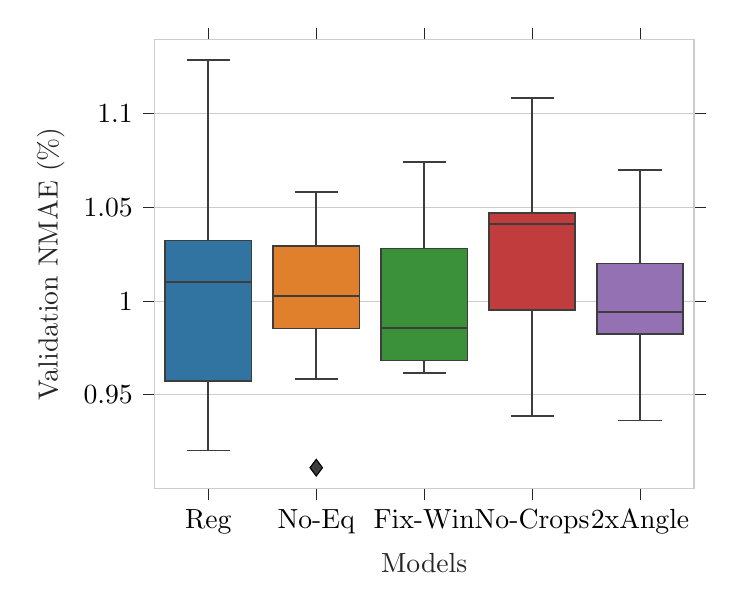
\begin{tikzpicture}

\definecolor{brown1926061}{RGB}{192,60,61}
\definecolor{darkslategray38}{RGB}{38,38,38}
\definecolor{darkslategray61}{RGB}{61,61,61}
\definecolor{lightgray204}{RGB}{204,204,204}
\definecolor{mediumpurple147113178}{RGB}{147,113,178}
\definecolor{peru22412844}{RGB}{224,128,44}
\definecolor{seagreen5814558}{RGB}{58,145,58}
\definecolor{steelblue49115161}{RGB}{49,115,161}

\begin{axis}[
axis line style={lightgray204},
tick align=outside,
x grid style={lightgray204},
xlabel=\textcolor{darkslategray38}{Models},
%xmajorticks=false,
xmin=-0.5, xmax=4.5,
xtick style={color=darkslategray38},
xtick={0,1,2,3,4},
xticklabels={Reg,No-Eq,Fix-Win,No-Crops,2xAngle},
y grid style={lightgray204},
ylabel=\textcolor{darkslategray38}{Validation NMAE (\%)},
ymajorgrids,
%ymajorticks=false,
ymin=0.900204116743225, ymax=1.13946537951647,
ytick style={color=darkslategray38}
]
\path [draw=darkslategray61, fill=steelblue49115161, semithick]
(axis cs:-0.4,0.957350027760654)
--(axis cs:0.4,0.957350027760654)
--(axis cs:0.4,1.03230924897689)
--(axis cs:-0.4,1.03230924897689)
--(axis cs:-0.4,0.957350027760654)
--cycle;
\path [draw=darkslategray61, fill=peru22412844, semithick]
(axis cs:0.6,0.985308041849543)
--(axis cs:1.4,0.985308041849543)
--(axis cs:1.4,1.02951164970211)
--(axis cs:0.6,1.02951164970211)
--(axis cs:0.6,0.985308041849543)
--cycle;
\path [draw=darkslategray61, fill=seagreen5814558, semithick]
(axis cs:1.6,0.968218953712826)
--(axis cs:2.4,0.968218953712826)
--(axis cs:2.4,1.02806765359832)
--(axis cs:1.6,1.02806765359832)
--(axis cs:1.6,0.968218953712826)
--cycle;
\path [draw=darkslategray61, fill=brown1926061, semithick]
(axis cs:2.6,0.995330950569849)
--(axis cs:3.4,0.995330950569849)
--(axis cs:3.4,1.04695238535411)
--(axis cs:2.6,1.04695238535411)
--(axis cs:2.6,0.995330950569849)
--cycle;
\path [draw=darkslategray61, fill=mediumpurple147113178, semithick]
(axis cs:3.6,0.982392603612466)
--(axis cs:4.4,0.982392603612466)
--(axis cs:4.4,1.02010316022565)
--(axis cs:3.6,1.02010316022565)
--(axis cs:3.6,0.982392603612466)
--cycle;
\addplot [semithick, darkslategray61]
table {%
0 0.957350027760654
0 0.920322989169918
};
\addplot [semithick, darkslategray61]
table {%
0 1.03230924897689
0 1.12858986757223
};
\addplot [semithick, darkslategray61]
table {%
-0.2 0.920322989169918
0.2 0.920322989169918
};
\addplot [semithick, darkslategray61]
table {%
-0.2 1.12858986757223
0.2 1.12858986757223
};
\addplot [semithick, darkslategray61]
table {%
1 0.985308041849543
1 0.958477547580371
};
\addplot [semithick, darkslategray61]
table {%
1 1.02951164970211
1 1.05823213403671
};
\addplot [semithick, darkslategray61]
table {%
0.8 0.958477547580371
1.2 0.958477547580371
};
\addplot [semithick, darkslategray61]
table {%
0.8 1.05823213403671
1.2 1.05823213403671
};
\addplot [black, mark=diamond*, mark size=3, mark options={solid,fill=darkslategray61}, only marks]
table {%
1 0.911079628687464
};
\addplot [semithick, darkslategray61]
table {%
2 0.968218953712826
2 0.961690867432787
};
\addplot [semithick, darkslategray61]
table {%
2 1.02806765359832
2 1.07409322367937
};
\addplot [semithick, darkslategray61]
table {%
1.8 0.961690867432787
2.2 0.961690867432787
};
\addplot [semithick, darkslategray61]
table {%
1.8 1.07409322367937
2.2 1.07409322367937
};
\addplot [semithick, darkslategray61]
table {%
3 0.995330950569849
3 0.938762616147096
};
\addplot [semithick, darkslategray61]
table {%
3 1.04695238535411
3 1.10849211870674
};
\addplot [semithick, darkslategray61]
table {%
2.8 0.938762616147096
3.2 0.938762616147096
};
\addplot [semithick, darkslategray61]
table {%
2.8 1.10849211870674
3.2 1.10849211870674
};
\addplot [semithick, darkslategray61]
table {%
4 0.982392603612466
4 0.93620586193136
};
\addplot [semithick, darkslategray61]
table {%
4 1.02010316022565
4 1.06984970159626
};
\addplot [semithick, darkslategray61]
table {%
3.8 0.93620586193136
4.2 0.93620586193136
};
\addplot [semithick, darkslategray61]
table {%
3.8 1.06984970159626
4.2 1.06984970159626
};
\addplot [semithick, darkslategray61]
table {%
-0.4 1.01029054533317
0.4 1.01029054533317
};
\addplot [semithick, darkslategray61]
table {%
0.6 1.00284380962488
1.4 1.00284380962488
};
\addplot [semithick, darkslategray61]
table {%
1.6 0.985471644034868
2.4 0.985471644034868
};
\addplot [semithick, darkslategray61]
table {%
2.6 1.04114435857173
3.4 1.04114435857173
};
\addplot [semithick, darkslategray61]
table {%
3.6 0.994276485894195
4.4 0.994276485894195
};
\end{axis}

\end{tikzpicture}

%\caption{Box diagram of the average NMAE (\%) of the density estimations in validation for the ablation study: the regression model considered (Reg) without equalization (No-Eq), a pre-processing with fixed window (Fix-Win), removing images taken from the central parts of the labeled samples (No-Crops), and limiting the maximum value of the random crop in DA (2xAngle). En each case 10 different trainings were run.}  
%\label{fig:AblationReg}
%\end{figure}

\begin{figure}[htp]
\centering
%\includegraphics[width=8cm]{../figsDef/boxRegressionValidationAblationNMAEV2}
% This file was created with tikzplotlib v0.10.1.
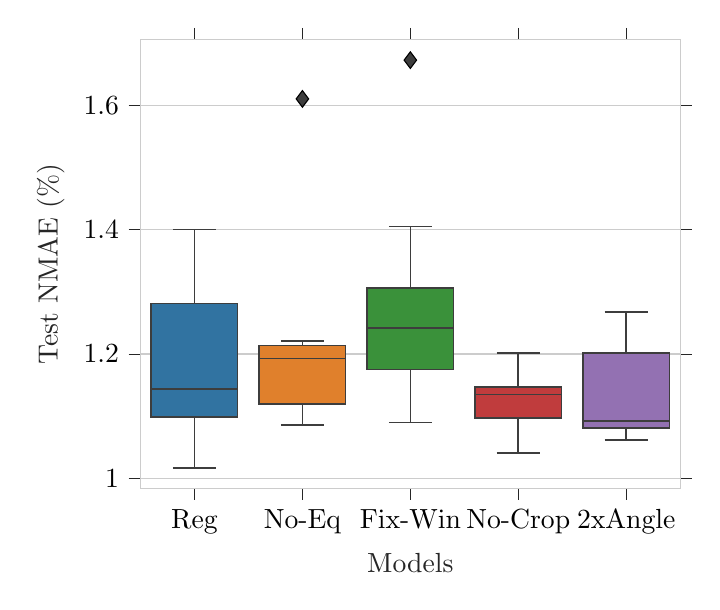
\begin{tikzpicture}

\definecolor{brown1926061}{RGB}{192,60,61}
\definecolor{darkslategray38}{RGB}{38,38,38}
\definecolor{darkslategray61}{RGB}{61,61,61}
\definecolor{lightgray204}{RGB}{204,204,204}
\definecolor{mediumpurple147113178}{RGB}{147,113,178}
\definecolor{peru22412844}{RGB}{224,128,44}
\definecolor{seagreen5814558}{RGB}{58,145,58}
\definecolor{steelblue49115161}{RGB}{49,115,161}

\begin{axis}[
axis line style={lightgray204},
tick align=outside,
x grid style={lightgray204},
xlabel=\textcolor{darkslategray38}{Models},
%xmajorticks=false,
xmin=-0.5, xmax=4.5,
xtick style={color=darkslategray38},
xtick={0,1,2,3,4},
xticklabels={Reg,No-Eq,Fix-Win,No-Crop,2xAngle},
y grid style={lightgray204},
ylabel=\textcolor{darkslategray38}{Test NMAE (\%)},
ymajorgrids,
%ymajorticks=false,
ymin=0.984116965331971, ymax=1.70584712622529,
ytick style={color=darkslategray38}
]
\path [draw=darkslategray61, fill=steelblue49115161, semithick]
(axis cs:-0.4,1.09855208092833)
--(axis cs:0.4,1.09855208092833)
--(axis cs:0.4,1.28099441629875)
--(axis cs:-0.4,1.28099441629875)
--(axis cs:-0.4,1.09855208092833)
--cycle;
\path [draw=darkslategray61, fill=peru22412844, semithick]
(axis cs:0.6,1.11949588552307)
--(axis cs:1.4,1.11949588552307)
--(axis cs:1.4,1.2138485491507)
--(axis cs:0.6,1.2138485491507)
--(axis cs:0.6,1.11949588552307)
--cycle;
\path [draw=darkslategray61, fill=seagreen5814558, semithick]
(axis cs:1.6,1.17499377156956)
--(axis cs:2.4,1.17499377156956)
--(axis cs:2.4,1.30582618907354)
--(axis cs:1.6,1.30582618907354)
--(axis cs:1.6,1.17499377156956)
--cycle;
\path [draw=darkslategray61, fill=brown1926061, semithick]
(axis cs:2.6,1.09700971152536)
--(axis cs:3.4,1.09700971152536)
--(axis cs:3.4,1.14710762198309)
--(axis cs:2.6,1.14710762198309)
--(axis cs:2.6,1.09700971152536)
--cycle;
\path [draw=darkslategray61, fill=mediumpurple147113178, semithick]
(axis cs:3.6,1.08039564137693)
--(axis cs:4.4,1.08039564137693)
--(axis cs:4.4,1.20129640303458)
--(axis cs:3.6,1.20129640303458)
--(axis cs:3.6,1.08039564137693)
--cycle;
\addplot [semithick, darkslategray61]
table {%
0 1.09855208092833
0 1.01692288173621
};
\addplot [semithick, darkslategray61]
table {%
0 1.28099441629875
0 1.40062535347857
};
\addplot [semithick, darkslategray61]
table {%
-0.2 1.01692288173621
0.2 1.01692288173621
};
\addplot [semithick, darkslategray61]
table {%
-0.2 1.40062535347857
0.2 1.40062535347857
};
\addplot [semithick, darkslategray61]
table {%
1 1.11949588552307
1 1.08517077122815
};
\addplot [semithick, darkslategray61]
table {%
1 1.2138485491507
1 1.22047296813172
};
\addplot [semithick, darkslategray61]
table {%
0.8 1.08517077122815
1.2 1.08517077122815
};
\addplot [semithick, darkslategray61]
table {%
0.8 1.22047296813172
1.2 1.22047296813172
};
\addplot [black, mark=diamond*, mark size=3, mark options={solid,fill=darkslategray61}, only marks]
table {%
1 1.61065048266513
};
\addplot [semithick, darkslategray61]
table {%
2 1.17499377156956
2 1.08959106212327
};
\addplot [semithick, darkslategray61]
table {%
2 1.30582618907354
2 1.40531247708067
};
\addplot [semithick, darkslategray61]
table {%
1.8 1.08959106212327
2.2 1.08959106212327
};
\addplot [semithick, darkslategray61]
table {%
1.8 1.40531247708067
2.2 1.40531247708067
};
\addplot [black, mark=diamond*, mark size=3, mark options={solid,fill=darkslategray61}, only marks]
table {%
2 1.67304120982105
};
\addplot [semithick, darkslategray61]
table {%
3 1.09700971152536
3 1.04021742731695
};
\addplot [semithick, darkslategray61]
table {%
3 1.14710762198309
3 1.20111650271348
};
\addplot [semithick, darkslategray61]
table {%
2.8 1.04021742731695
3.2 1.04021742731695
};
\addplot [semithick, darkslategray61]
table {%
2.8 1.20111650271348
3.2 1.20111650271348
};
\addplot [semithick, darkslategray61]
table {%
4 1.08039564137693
4 1.06177310400461
};
\addplot [semithick, darkslategray61]
table {%
4 1.20129640303458
4 1.26736836015092
};
\addplot [semithick, darkslategray61]
table {%
3.8 1.06177310400461
4.2 1.06177310400461
};
\addplot [semithick, darkslategray61]
table {%
3.8 1.26736836015092
4.2 1.26736836015092
};
\addplot [semithick, darkslategray61]
table {%
-0.4 1.14381436197598
0.4 1.14381436197598
};
\addplot [semithick, darkslategray61]
table {%
0.6 1.19247745757901
1.4 1.19247745757901
};
\addplot [semithick, darkslategray61]
table {%
1.6 1.24191562182427
2.4 1.24191562182427
};
\addplot [semithick, darkslategray61]
table {%
2.6 1.13457615202707
3.4 1.13457615202707
};
\addplot [semithick, darkslategray61]
table {%
3.6 1.09212248244153
4.4 1.09212248244153
};
\end{axis}

\end{tikzpicture}

\caption{Box diagram of the average NMAE (\%) of the density estimations for the test dataset in the ablation study: the regression model considered (Reg) without equalization (No-Eq), a pre-processing with fixed window (Fix-Win), removing images taken from the central parts of the labeled samples (No-Crop), and limiting the maximum value of the random angle in DA (2xAngle). In each case, 10 different trainings were run. Outliers are represented with diamonds. }  
\label{fig:AblationRegTest}
\end{figure}

\section{Semi-Supervised Training}\label{sec:SS}

%In the canvas analysis, we aim at providing the curator with the best solution. In \cite{Bejarano2023} it was outlined that in areas with poor contrast, usually saturated zones, the FT outperformed the segmentation DL approach. We observed that the regression DL quite improved the density estimation results of the segmentation. 

To improve the estimation in these scenarios, we propose a semi-supervised (SS) approach, see Alg. \ref{alg:SS}. The key of this SS method is to create, given a canvas to be analyzed, a dataset of patches where the FT and the regression DL provide similar estimates. Then, train the regression DL solution for some epochs with this dataset. This can be also viewed as a transfer learning, see \cite{Aradillas21} and references therein, where the starting point is the already trained inception VGG regression DL and we re-train it with this new dataset generated for the processed canvas. The main advantage is that we do not need to label any of the new images, as we use those where the FT and initial regression DL agree. After the SS algorithm, the refined model at the output is used to estimate the thread densities. Note that with this SS approach, we expect to improve the solution there were the FT provide good enough solutions and no improvement at all otherwise.

\begin{algorithm}
\caption{Semi-Supervised Learning}\label{alg:SS}
\textbf{Input:} Pre-processed patches and counts (predictions), trained regression DL model.
\begin{algorithmic}[1]
\State  Create a dataset with input images where the error in the estimation of FT and regression DL in both vertical and horizontal threads is under 4\%. 
% error es absoluto normalizado y la etiqueta se toma la de DL
%
%REVISAR ESTO
%
%For all the pre-processed crops in the painting, it is checked if the difference between the count predicted by the ANN and the count obtained by FT is less than 4\%. In this case, each crop is saved as a sample (and the count as a label) for semi-supervised learning. Correspondence between ANN prediction and FT is checked in both the vertical count and the horizontal count.
\State 
To keep complexity bounded set a limit for the size, $N$, by randomly sampling instances in the created dataset.
%Of all the samples generated, a maximum number is saved for each row of the image, so as not to generate an uncontrolled number of samples. In our case, using an Intel Xeon E5-2630 v4 40 CPU Cores + 16GB Tesla P100 GPU, we have saved a maximum of 60,000 crops per painting randomly distributed among the rows.
\State Randomly split the dataset into 70\% and 30\% subsets, for training and validation, respectively.% is destined for training and the remaining 30\% for validation. The distribution in both sets is also done randomly.
%Of all the samples generated, 70\% is destined for training and the remaining 30\% for validation. The distribution in both sets is also done randomly.
\State Train the input model, with given weights as initial values, using the new dataset.  
%In this stage of fine tuning, we set a low learning rate of $1e-4$, a maximum of 10 epochs and a patience of only 1 epoch. In our tests we have verified that learning generally converges before 6 epochs. 
%The reason for refining the weights is to get the network to learn in more detail the fabric it is dealing with in each particular experiment.
%\State The weights for the epoch with the least loss in validation are saved. The loss function used is the same as that used for training the model, NMAE. When the fine tuning is finished, these weights are uploaded to the network to make the new predictions.
%\State Finally, all the pre-processed crops of the painting are reviewed and the value of the vertical and horizontal count is obtained using the refined model.
\end{algorithmic}
\textbf{Output:} The input model with the values of the new weights.
\end{algorithm}

The proposed SS algorithm was applied row-wise as follows. The trained Reg-VGG and the FT were applied to the set of $F$ rows to obtain up to $N=60,000$ samples. These images were used to train the Reg-VGG initialized to the weights obtained in Sec. \ref{sec:train} with a learning rate set to $10^{-3}$, early stopping with 3 epochs of patience for a maximum of 20 epochs, and the NMAE as loss function. The last three layers in the dense network were frozen. % Learning usually converges after 6 epochs.
%
We applied this SS regression DL approach to the four canvases in the validation set to further reduce the NMAE, from 0.92\% to 0.90\%. In test, the reduction is from 1.01\% to 0.94\%. 


For the sake of completeness, in  Fig. \ref{fig:TestSamples}.a we include the result of the normalized absolute error (NAE) in the vertical and horizontal density estimation for each test image and the best Reg model, i.e., the Reg-VGG with the lowest validation error, when SS is applied. In Fig. \ref{fig:TestSamples}.b we include the errors for the regression DL with no SS. In Fig. \ref{fig:TestSamples}.c and Fig. \ref{fig:TestSamples}.d we depict the error for the Inc-Dice as in \cite{Bejarano2023}  and the FT, respectively. The error of the FT is quite large. The first 28 images correspond to the same canvas and the method is unable to provide a valid estimation. Compared to the segmentation DL, the error of the regression DL decreases for most of the test samples. When using SS the errors are further reduced. Only two test samples exhibit an error greater than 5\% using the new regression approach. These errors could correspond to samples that were difficult to label, as threads were not easily observed. 


\begin{figure*}[htp]
\centering
\begin{tabular}{c}
% \includegraphics[width=11cm]{../figsDef/JUNTOS.png} \\
% This file was created with tikzplotlib v0.10.1.
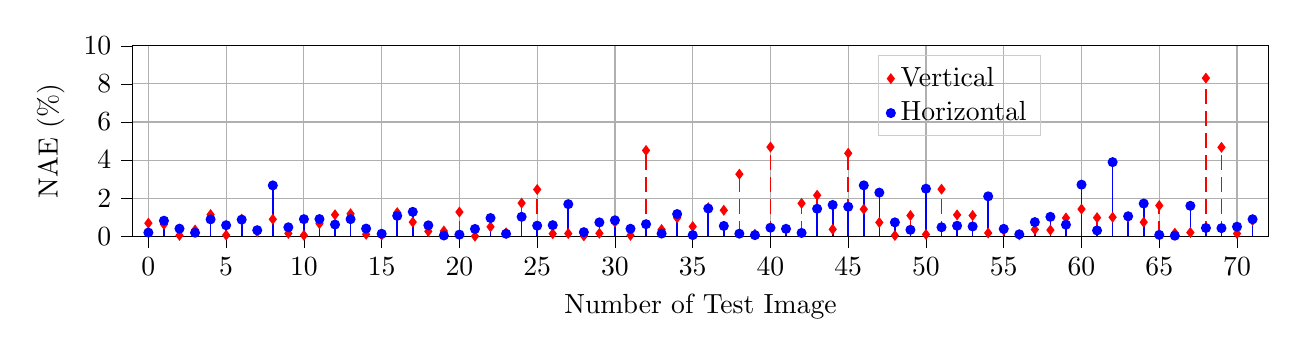
\begin{tikzpicture}

\definecolor{crimson2143940}{RGB}{214,39,40}
\definecolor{darkgray176}{RGB}{176,176,176}
\definecolor{lightgray204}{RGB}{204,204,204}

\begin{axis}[
width = 16cm,
height = 4cm,
legend cell align={left},
legend style={fill=none, text opacity=1, draw=lightgray204, at={(0.8,0.95)}},
tick align=outside,
tick pos=left,
x grid style={darkgray176},
xlabel={Number of Test Image},
xmajorgrids,
xmin=-1, xmax=72,
xtick style={color=black},
y grid style={darkgray176},
ylabel={NAE (\%)},
ymajorgrids,
ymin=0, ymax=10,
ytick style={color=black}
]
\path [draw=red, semithick, dash pattern=on 5.55pt off 2.4pt]
(axis cs:0,0)
--(axis cs:0,0.686254322528839);

\path [draw=red, semithick, dash pattern=on 5.55pt off 2.4pt]
(axis cs:1,0)
--(axis cs:1,0.618949472904205);

\path [draw=red, semithick, dash pattern=on 5.55pt off 2.4pt]
(axis cs:2,0)
--(axis cs:2,0.0461614578962326);

\path [draw=red, semithick, dash pattern=on 5.55pt off 2.4pt]
(axis cs:3,0)
--(axis cs:3,0.328216671943665);

\path [draw=red, semithick, dash pattern=on 5.55pt off 2.4pt]
(axis cs:4,0)
--(axis cs:4,1.14099705219269);

\path [draw=red, semithick, dash pattern=on 5.55pt off 2.4pt]
(axis cs:5,0)
--(axis cs:5,0.0591133795678616);

\path [draw=red, semithick, dash pattern=on 5.55pt off 2.4pt]
(axis cs:6,0)
--(axis cs:6,0.899910628795624);

\path [draw=red, semithick, dash pattern=on 5.55pt off 2.4pt]
(axis cs:7,0)
--(axis cs:7,0.229798600077629);

\path [draw=red, semithick, dash pattern=on 5.55pt off 2.4pt]
(axis cs:8,0)
--(axis cs:8,0.892645955085754);

\path [draw=red, semithick, dash pattern=on 5.55pt off 2.4pt]
(axis cs:9,0)
--(axis cs:9,0.148607403039932);

\path [draw=red, semithick, dash pattern=on 5.55pt off 2.4pt]
(axis cs:10,0)
--(axis cs:10,0.0516327731311321);

\path [draw=red, semithick, dash pattern=on 5.55pt off 2.4pt]
(axis cs:11,0)
--(axis cs:11,0.66338175535202);

\path [draw=red, semithick, dash pattern=on 5.55pt off 2.4pt]
(axis cs:12,0)
--(axis cs:12,1.12749004364014);

\path [draw=red, semithick, dash pattern=on 5.55pt off 2.4pt]
(axis cs:13,0)
--(axis cs:13,1.17979669570923);

\path [draw=red, semithick, dash pattern=on 5.55pt off 2.4pt]
(axis cs:14,0)
--(axis cs:14,0.0993922129273415);

\path [draw=red, semithick, dash pattern=on 5.55pt off 2.4pt]
(axis cs:15,0)
--(axis cs:15,0.0609384141862392);

\path [draw=red, semithick, dash pattern=on 5.55pt off 2.4pt]
(axis cs:16,0)
--(axis cs:16,1.24049186706543);

\path [draw=red, semithick, dash pattern=on 5.55pt off 2.4pt]
(axis cs:17,0)
--(axis cs:17,0.742619335651398);

\path [draw=red, semithick, dash pattern=on 5.55pt off 2.4pt]
(axis cs:18,0)
--(axis cs:18,0.254823297262192);

\path [draw=red, semithick, dash pattern=on 5.55pt off 2.4pt]
(axis cs:19,0)
--(axis cs:19,0.274400681257248);

\path [draw=red, semithick, dash pattern=on 5.55pt off 2.4pt]
(axis cs:20,0)
--(axis cs:20,1.27164971828461);

\path [draw=red, semithick, dash pattern=on 5.55pt off 2.4pt]
(axis cs:21,0)
--(axis cs:21,0.00262976996600628);

\path [draw=red, semithick, dash pattern=on 5.55pt off 2.4pt]
(axis cs:22,0)
--(axis cs:22,0.496395945549011);

\path [draw=red, semithick, dash pattern=on 5.55pt off 2.4pt]
(axis cs:23,0)
--(axis cs:23,0.18026776611805);

\path [draw=red, semithick, dash pattern=on 5.55pt off 2.4pt]
(axis cs:24,0)
--(axis cs:24,1.74043202400208);

\path [draw=red, semithick, dash pattern=on 5.55pt off 2.4pt]
(axis cs:25,0)
--(axis cs:25,2.45278525352478);

\path [draw=red, semithick, dash pattern=on 5.55pt off 2.4pt]
(axis cs:26,0)
--(axis cs:26,0.133196398615837);

\path [draw=red, semithick, dash pattern=on 5.55pt off 2.4pt]
(axis cs:27,0)
--(axis cs:27,0.142650872468948);

\path [draw=red, semithick, dash pattern=on 5.55pt off 2.4pt]
(axis cs:28,0)
--(axis cs:28,0.0169488042593002);

\path [draw=red, semithick, dash pattern=on 5.55pt off 2.4pt]
(axis cs:29,0)
--(axis cs:29,0.156440660357475);

\path [draw=red, semithick, dash pattern=on 5.55pt off 2.4pt]
(axis cs:30,0)
--(axis cs:30,0.740674018859863);

\path [draw=red, semithick, dash pattern=on 5.55pt off 2.4pt]
(axis cs:31,0)
--(axis cs:31,0.0488951466977596);

\path [draw=red, semithick, dash pattern=on 5.55pt off 2.4pt]
(axis cs:32,0)
--(axis cs:32,4.50450229644775);

\path [draw=red, semithick, dash pattern=on 5.55pt off 2.4pt]
(axis cs:33,0)
--(axis cs:33,0.351666539907455);

\path [draw=red, semithick, dash pattern=on 5.55pt off 2.4pt]
(axis cs:34,0)
--(axis cs:34,0.96680748462677);

\path [draw=red, semithick, dash pattern=on 5.55pt off 2.4pt]
(axis cs:35,0)
--(axis cs:35,0.509925842285156);

\path [draw=red, semithick, dash pattern=on 5.55pt off 2.4pt]
(axis cs:36,0)
--(axis cs:36,1.49655377864838);

\path [draw=red, semithick, dash pattern=on 5.55pt off 2.4pt]
(axis cs:37,0)
--(axis cs:37,1.36532974243164);

\path [draw=red, semithick, dash pattern=on 5.55pt off 2.4pt]
(axis cs:38,0)
--(axis cs:38,3.25969934463501);

\path [draw=red, semithick, dash pattern=on 5.55pt off 2.4pt]
(axis cs:39,0)
--(axis cs:39,0.107412248849869);

\path [draw=red, semithick, dash pattern=on 5.55pt off 2.4pt]
(axis cs:40,0)
--(axis cs:40,4.68319988250732);

\path [draw=red, semithick, dash pattern=on 5.55pt off 2.4pt]
(axis cs:41,0)
--(axis cs:41,0.379445880651474);

\path [draw=red, semithick, dash pattern=on 5.55pt off 2.4pt]
(axis cs:42,0)
--(axis cs:42,1.72759962081909);

\path [draw=red, semithick, dash pattern=on 5.55pt off 2.4pt]
(axis cs:43,0)
--(axis cs:43,2.15176224708557);

\path [draw=red, semithick, dash pattern=on 5.55pt off 2.4pt]
(axis cs:44,0)
--(axis cs:44,0.363650292158127);

\path [draw=red, semithick, dash pattern=on 5.55pt off 2.4pt]
(axis cs:45,0)
--(axis cs:45,4.35523653030396);

\path [draw=red, semithick, dash pattern=on 5.55pt off 2.4pt]
(axis cs:46,0)
--(axis cs:46,1.41879236698151);

\path [draw=red, semithick, dash pattern=on 5.55pt off 2.4pt]
(axis cs:47,0)
--(axis cs:47,0.72240823507309);

\path [draw=red, semithick, dash pattern=on 5.55pt off 2.4pt]
(axis cs:48,0)
--(axis cs:48,0.0401907078921795);

\path [draw=red, semithick, dash pattern=on 5.55pt off 2.4pt]
(axis cs:49,0)
--(axis cs:49,1.08979785442352);

\path [draw=red, semithick, dash pattern=on 5.55pt off 2.4pt]
(axis cs:50,0)
--(axis cs:50,0.0973271951079369);

\path [draw=red, semithick, dash pattern=on 5.55pt off 2.4pt]
(axis cs:51,0)
--(axis cs:51,2.47079277038574);

\path [draw=red, semithick, dash pattern=on 5.55pt off 2.4pt]
(axis cs:52,0)
--(axis cs:52,1.12119293212891);

\path [draw=red, semithick, dash pattern=on 5.55pt off 2.4pt]
(axis cs:53,0)
--(axis cs:53,1.08939123153687);

\path [draw=red, semithick, dash pattern=on 5.55pt off 2.4pt]
(axis cs:54,0)
--(axis cs:54,0.169967979192734);

\path [draw=red, semithick, dash pattern=on 5.55pt off 2.4pt]
(axis cs:55,0)
--(axis cs:55,0.31207337975502);

\path [draw=red, semithick, dash pattern=on 5.55pt off 2.4pt]
(axis cs:56,0)
--(axis cs:56,0.0732015147805214);

\path [draw=red, semithick, dash pattern=on 5.55pt off 2.4pt]
(axis cs:57,0)
--(axis cs:57,0.352627903223038);

\path [draw=red, semithick, dash pattern=on 5.55pt off 2.4pt]
(axis cs:58,0)
--(axis cs:58,0.326722383499146);

\path [draw=red, semithick, dash pattern=on 5.55pt off 2.4pt]
(axis cs:59,0)
--(axis cs:59,0.961142659187317);

\path [draw=red, semithick, dash pattern=on 5.55pt off 2.4pt]
(axis cs:60,0)
--(axis cs:60,1.42522990703583);

\path [draw=red, semithick, dash pattern=on 5.55pt off 2.4pt]
(axis cs:61,0)
--(axis cs:61,0.975054144859314);

\path [draw=red, semithick, dash pattern=on 5.55pt off 2.4pt]
(axis cs:62,0)
--(axis cs:62,0.997181057929993);

\path [draw=red, semithick, dash pattern=on 5.55pt off 2.4pt]
(axis cs:63,0)
--(axis cs:63,1.00286984443665);

\path [draw=red, semithick, dash pattern=on 5.55pt off 2.4pt]
(axis cs:64,0)
--(axis cs:64,0.736421883106232);

\path [draw=red, semithick, dash pattern=on 5.55pt off 2.4pt]
(axis cs:65,0)
--(axis cs:65,1.61220109462738);

\path [draw=red, semithick, dash pattern=on 5.55pt off 2.4pt]
(axis cs:66,0)
--(axis cs:66,0.159175023436546);

\path [draw=red, semithick, dash pattern=on 5.55pt off 2.4pt]
(axis cs:67,0)
--(axis cs:67,0.197410121560097);

\path [draw=red, semithick, dash pattern=on 5.55pt off 2.4pt]
(axis cs:68,0)
--(axis cs:68,8.30304718017578);

\path [draw=red, semithick, dash pattern=on 5.55pt off 2.4pt]
(axis cs:69,0)
--(axis cs:69,4.66914176940918);

\path [draw=red, semithick, dash pattern=on 5.55pt off 2.4pt]
(axis cs:70,0)
--(axis cs:70,0.142979219555855);

\path [draw=red, semithick, dash pattern=on 5.55pt off 2.4pt]
(axis cs:71,0)
--(axis cs:71,0.829527735710144);

\path [draw=blue, semithick]
(axis cs:0,0)
--(axis cs:0,0.192356362938881);

\path [draw=blue, semithick]
(axis cs:1,0)
--(axis cs:1,0.814959228038788);

\path [draw=blue, semithick]
(axis cs:2,0)
--(axis cs:2,0.397479385137558);

\path [draw=blue, semithick]
(axis cs:3,0)
--(axis cs:3,0.185900434851646);

\path [draw=blue, semithick]
(axis cs:4,0)
--(axis cs:4,0.886518120765686);

\path [draw=blue, semithick]
(axis cs:5,0)
--(axis cs:5,0.578838884830475);

\path [draw=blue, semithick]
(axis cs:6,0)
--(axis cs:6,0.872652530670166);

\path [draw=blue, semithick]
(axis cs:7,0)
--(axis cs:7,0.317274868488312);

\path [draw=blue, semithick]
(axis cs:8,0)
--(axis cs:8,2.66949391365051);

\path [draw=blue, semithick]
(axis cs:9,0)
--(axis cs:9,0.470038175582886);

\path [draw=blue, semithick]
(axis cs:10,0)
--(axis cs:10,0.897140800952911);

\path [draw=blue, semithick]
(axis cs:11,0)
--(axis cs:11,0.901799559593201);

\path [draw=blue, semithick]
(axis cs:12,0)
--(axis cs:12,0.615128695964813);

\path [draw=blue, semithick]
(axis cs:13,0)
--(axis cs:13,0.897373378276825);

\path [draw=blue, semithick]
(axis cs:14,0)
--(axis cs:14,0.402732878923416);

\path [draw=blue, semithick]
(axis cs:15,0)
--(axis cs:15,0.129007309675217);

\path [draw=blue, semithick]
(axis cs:16,0)
--(axis cs:16,1.07197463512421);

\path [draw=blue, semithick]
(axis cs:17,0)
--(axis cs:17,1.28065288066864);

\path [draw=blue, semithick]
(axis cs:18,0)
--(axis cs:18,0.572273731231689);

\path [draw=blue, semithick]
(axis cs:19,0)
--(axis cs:19,0.0398504212498665);

\path [draw=blue, semithick]
(axis cs:20,0)
--(axis cs:20,0.0846728533506393);

\path [draw=blue, semithick]
(axis cs:21,0)
--(axis cs:21,0.382970154285431);

\path [draw=blue, semithick]
(axis cs:22,0)
--(axis cs:22,0.956841349601746);

\path [draw=blue, semithick]
(axis cs:23,0)
--(axis cs:23,0.12898887693882);

\path [draw=blue, semithick]
(axis cs:24,0)
--(axis cs:24,1.02006936073303);

\path [draw=blue, semithick]
(axis cs:25,0)
--(axis cs:25,0.555101871490479);

\path [draw=blue, semithick]
(axis cs:26,0)
--(axis cs:26,0.582029402256012);

\path [draw=blue, semithick]
(axis cs:27,0)
--(axis cs:27,1.6847882270813);

\path [draw=blue, semithick]
(axis cs:28,0)
--(axis cs:28,0.214249178767204);

\path [draw=blue, semithick]
(axis cs:29,0)
--(axis cs:29,0.727674007415771);

\path [draw=blue, semithick]
(axis cs:30,0)
--(axis cs:30,0.837226867675781);

\path [draw=blue, semithick]
(axis cs:31,0)
--(axis cs:31,0.392680048942566);

\path [draw=blue, semithick]
(axis cs:32,0)
--(axis cs:32,0.633628189563751);

\path [draw=blue, semithick]
(axis cs:33,0)
--(axis cs:33,0.141428485512733);

\path [draw=blue, semithick]
(axis cs:34,0)
--(axis cs:34,1.16498577594757);

\path [draw=blue, semithick]
(axis cs:35,0)
--(axis cs:35,0.0602010525763035);

\path [draw=blue, semithick]
(axis cs:36,0)
--(axis cs:36,1.45564258098602);

\path [draw=blue, semithick]
(axis cs:37,0)
--(axis cs:37,0.540462732315063);

\path [draw=blue, semithick]
(axis cs:38,0)
--(axis cs:38,0.134616911411285);

\path [draw=blue, semithick]
(axis cs:39,0)
--(axis cs:39,0.0595284178853035);

\path [draw=blue, semithick]
(axis cs:40,0)
--(axis cs:40,0.447664737701416);

\path [draw=blue, semithick]
(axis cs:41,0)
--(axis cs:41,0.388050377368927);

\path [draw=blue, semithick]
(axis cs:42,0)
--(axis cs:42,0.1733727902174);

\path [draw=blue, semithick]
(axis cs:43,0)
--(axis cs:43,1.44400274753571);

\path [draw=blue, semithick]
(axis cs:44,0)
--(axis cs:44,1.64304912090302);

\path [draw=blue, semithick]
(axis cs:45,0)
--(axis cs:45,1.54892349243164);

\path [draw=blue, semithick]
(axis cs:46,0)
--(axis cs:46,2.672287940979);

\path [draw=blue, semithick]
(axis cs:47,0)
--(axis cs:47,2.29101586341858);

\path [draw=blue, semithick]
(axis cs:48,0)
--(axis cs:48,0.727793455123901);

\path [draw=blue, semithick]
(axis cs:49,0)
--(axis cs:49,0.337266951799393);

\path [draw=blue, semithick]
(axis cs:50,0)
--(axis cs:50,2.49650001525879);

\path [draw=blue, semithick]
(axis cs:51,0)
--(axis cs:51,0.472472876310349);

\path [draw=blue, semithick]
(axis cs:52,0)
--(axis cs:52,0.550615131855011);

\path [draw=blue, semithick]
(axis cs:53,0)
--(axis cs:53,0.5145143866539);

\path [draw=blue, semithick]
(axis cs:54,0)
--(axis cs:54,2.09619879722595);

\path [draw=blue, semithick]
(axis cs:55,0)
--(axis cs:55,0.387734919786453);

\path [draw=blue, semithick]
(axis cs:56,0)
--(axis cs:56,0.101625882089138);

\path [draw=blue, semithick]
(axis cs:57,0)
--(axis cs:57,0.7415811419487);

\path [draw=blue, semithick]
(axis cs:58,0)
--(axis cs:58,1.01858103275299);

\path [draw=blue, semithick]
(axis cs:59,0)
--(axis cs:59,0.605757355690002);

\path [draw=blue, semithick]
(axis cs:60,0)
--(axis cs:60,2.70938777923584);

\path [draw=blue, semithick]
(axis cs:61,0)
--(axis cs:61,0.304962038993835);

\path [draw=blue, semithick]
(axis cs:62,0)
--(axis cs:62,3.89161229133606);

\path [draw=blue, semithick]
(axis cs:63,0)
--(axis cs:63,1.04899883270264);

\path [draw=blue, semithick]
(axis cs:64,0)
--(axis cs:64,1.71723234653473);

\path [draw=blue, semithick]
(axis cs:65,0)
--(axis cs:65,0.0710364282131195);

\path [draw=blue, semithick]
(axis cs:66,0)
--(axis cs:66,0.0298584699630737);

\path [draw=blue, semithick]
(axis cs:67,0)
--(axis cs:67,1.59748363494873);

\path [draw=blue, semithick]
(axis cs:68,0)
--(axis cs:68,0.434109508991241);

\path [draw=blue, semithick]
(axis cs:69,0)
--(axis cs:69,0.425687521696091);

\path [draw=blue, semithick]
(axis cs:70,0)
--(axis cs:70,0.501553416252136);

\path [draw=blue, semithick]
(axis cs:71,0)
--(axis cs:71,0.891443729400635);

\addplot [semithick, red, mark=diamond*, mark size=1.5, mark options={solid}, only marks]
table {%
0 0.686254322528839
1 0.618949472904205
2 0.0461614578962326
3 0.328216671943665
4 1.14099705219269
5 0.0591133795678616
6 0.899910628795624
7 0.229798600077629
8 0.892645955085754
9 0.148607403039932
10 0.0516327731311321
11 0.66338175535202
12 1.12749004364014
13 1.17979669570923
14 0.0993922129273415
15 0.0609384141862392
16 1.24049186706543
17 0.742619335651398
18 0.254823297262192
19 0.274400681257248
20 1.27164971828461
21 0.00262976996600628
22 0.496395945549011
23 0.18026776611805
24 1.74043202400208
25 2.45278525352478
26 0.133196398615837
27 0.142650872468948
28 0.0169488042593002
29 0.156440660357475
30 0.740674018859863
31 0.0488951466977596
32 4.50450229644775
33 0.351666539907455
34 0.96680748462677
35 0.509925842285156
36 1.49655377864838
37 1.36532974243164
38 3.25969934463501
39 0.107412248849869
40 4.68319988250732
41 0.379445880651474
42 1.72759962081909
43 2.15176224708557
44 0.363650292158127
45 4.35523653030396
46 1.41879236698151
47 0.72240823507309
48 0.0401907078921795
49 1.08979785442352
50 0.0973271951079369
51 2.47079277038574
52 1.12119293212891
53 1.08939123153687
54 0.169967979192734
55 0.31207337975502
56 0.0732015147805214
57 0.352627903223038
58 0.326722383499146
59 0.961142659187317
60 1.42522990703583
61 0.975054144859314
62 0.997181057929993
63 1.00286984443665
64 0.736421883106232
65 1.61220109462738
66 0.159175023436546
67 0.197410121560097
68 8.30304718017578
69 4.66914176940918
70 0.142979219555855
71 0.829527735710144
};\addlegendentry{Vertical}
\addplot [semithick, blue, mark=*, mark size=1.5, mark options={solid}, only marks]
table {%
0 0.192356362938881
1 0.814959228038788
2 0.397479385137558
3 0.185900434851646
4 0.886518120765686
5 0.578838884830475
6 0.872652530670166
7 0.317274868488312
8 2.66949391365051
9 0.470038175582886
10 0.897140800952911
11 0.901799559593201
12 0.615128695964813
13 0.897373378276825
14 0.402732878923416
15 0.129007309675217
16 1.07197463512421
17 1.28065288066864
18 0.572273731231689
19 0.0398504212498665
20 0.0846728533506393
21 0.382970154285431
22 0.956841349601746
23 0.12898887693882
24 1.02006936073303
25 0.555101871490479
26 0.582029402256012
27 1.6847882270813
28 0.214249178767204
29 0.727674007415771
30 0.837226867675781
31 0.392680048942566
32 0.633628189563751
33 0.141428485512733
34 1.16498577594757
35 0.0602010525763035
36 1.45564258098602
37 0.540462732315063
38 0.134616911411285
39 0.0595284178853035
40 0.447664737701416
41 0.388050377368927
42 0.1733727902174
43 1.44400274753571
44 1.64304912090302
45 1.54892349243164
46 2.672287940979
47 2.29101586341858
48 0.727793455123901
49 0.337266951799393
50 2.49650001525879
51 0.472472876310349
52 0.550615131855011
53 0.5145143866539
54 2.09619879722595
55 0.387734919786453
56 0.101625882089138
57 0.7415811419487
58 1.01858103275299
59 0.605757355690002
60 2.70938777923584
61 0.304962038993835
62 3.89161229133606
63 1.04899883270264
64 1.71723234653473
65 0.0710364282131195
66 0.0298584699630737
67 1.59748363494873
68 0.434109508991241
69 0.425687521696091
70 0.501553416252136
71 0.891443729400635
};\addlegendentry{Horizontal}
\end{axis}
\end{tikzpicture} \\
 (a) \\
% This file was created with tikzplotlib v0.10.1.
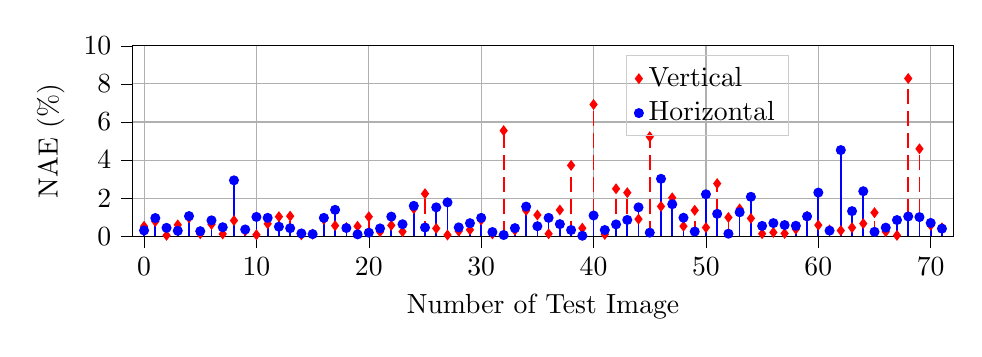
\begin{tikzpicture}

\definecolor{crimson2143940}{RGB}{214,39,40}
\definecolor{darkgray176}{RGB}{176,176,176}
\definecolor{lightgray204}{RGB}{204,204,204}

\begin{axis}[
width = 12cm,
height = 4cm,
legend cell align={left},
legend style={fill=none, text opacity=1, draw=lightgray204, at={(0.8,0.95)}},
tick align=outside,
tick pos=left,
x grid style={darkgray176},
xlabel={Number of Test Image},
xmajorgrids,
xmin=-1, xmax=72,
xtick style={color=black},
y grid style={darkgray176},
ylabel={NAE (\%)},
ymajorgrids,
ymin=0, ymax=10,
ytick style={color=black}
]
\path [draw=red, semithick, dash pattern=on 5.55pt off 2.4pt]
(axis cs:0,0)
--(axis cs:0,0.521718621253967);

\path [draw=red, semithick, dash pattern=on 5.55pt off 2.4pt]
(axis cs:1,0)
--(axis cs:1,0.775294184684753);

\path [draw=red, semithick, dash pattern=on 5.55pt off 2.4pt]
(axis cs:2,0)
--(axis cs:2,0.0469293147325516);

\path [draw=red, semithick, dash pattern=on 5.55pt off 2.4pt]
(axis cs:3,0)
--(axis cs:3,0.597368955612183);

\path [draw=red, semithick, dash pattern=on 5.55pt off 2.4pt]
(axis cs:4,0)
--(axis cs:4,0.964810073375702);

\path [draw=red, semithick, dash pattern=on 5.55pt off 2.4pt]
(axis cs:5,0)
--(axis cs:5,0.13081781566143);

\path [draw=red, semithick, dash pattern=on 5.55pt off 2.4pt]
(axis cs:6,0)
--(axis cs:6,0.62456613779068);

\path [draw=red, semithick, dash pattern=on 5.55pt off 2.4pt]
(axis cs:7,0)
--(axis cs:7,0.118860848248005);

\path [draw=red, semithick, dash pattern=on 5.55pt off 2.4pt]
(axis cs:8,0)
--(axis cs:8,0.822715640068054);

\path [draw=red, semithick, dash pattern=on 5.55pt off 2.4pt]
(axis cs:9,0)
--(axis cs:9,0.280089408159256);

\path [draw=red, semithick, dash pattern=on 5.55pt off 2.4pt]
(axis cs:10,0)
--(axis cs:10,0.0779043659567833);

\path [draw=red, semithick, dash pattern=on 5.55pt off 2.4pt]
(axis cs:11,0)
--(axis cs:11,0.65388035774231);

\path [draw=red, semithick, dash pattern=on 5.55pt off 2.4pt]
(axis cs:12,0)
--(axis cs:12,1.02718818187714);

\path [draw=red, semithick, dash pattern=on 5.55pt off 2.4pt]
(axis cs:13,0)
--(axis cs:13,1.05518460273743);

\path [draw=red, semithick, dash pattern=on 5.55pt off 2.4pt]
(axis cs:14,0)
--(axis cs:14,0.0773139670491219);

\path [draw=red, semithick, dash pattern=on 5.55pt off 2.4pt]
(axis cs:15,0)
--(axis cs:15,0.109499298036098);

\path [draw=red, semithick, dash pattern=on 5.55pt off 2.4pt]
(axis cs:16,0)
--(axis cs:16,0.881250977516174);

\path [draw=red, semithick, dash pattern=on 5.55pt off 2.4pt]
(axis cs:17,0)
--(axis cs:17,0.5565584897995);

\path [draw=red, semithick, dash pattern=on 5.55pt off 2.4pt]
(axis cs:18,0)
--(axis cs:18,0.455308049917221);

\path [draw=red, semithick, dash pattern=on 5.55pt off 2.4pt]
(axis cs:19,0)
--(axis cs:19,0.524994611740112);

\path [draw=red, semithick, dash pattern=on 5.55pt off 2.4pt]
(axis cs:20,0)
--(axis cs:20,1.02424097061157);

\path [draw=red, semithick, dash pattern=on 5.55pt off 2.4pt]
(axis cs:21,0)
--(axis cs:21,0.233435422182083);

\path [draw=red, semithick, dash pattern=on 5.55pt off 2.4pt]
(axis cs:22,0)
--(axis cs:22,0.57281631231308);

\path [draw=red, semithick, dash pattern=on 5.55pt off 2.4pt]
(axis cs:23,0)
--(axis cs:23,0.24091212451458);

\path [draw=red, semithick, dash pattern=on 5.55pt off 2.4pt]
(axis cs:24,0)
--(axis cs:24,1.45005226135254);

\path [draw=red, semithick, dash pattern=on 5.55pt off 2.4pt]
(axis cs:25,0)
--(axis cs:25,2.23428821563721);

\path [draw=red, semithick, dash pattern=on 5.55pt off 2.4pt]
(axis cs:26,0)
--(axis cs:26,0.409771323204041);

\path [draw=red, semithick, dash pattern=on 5.55pt off 2.4pt]
(axis cs:27,0)
--(axis cs:27,0.0655004978179932);

\path [draw=red, semithick, dash pattern=on 5.55pt off 2.4pt]
(axis cs:28,0)
--(axis cs:28,0.265586405992508);

\path [draw=red, semithick, dash pattern=on 5.55pt off 2.4pt]
(axis cs:29,0)
--(axis cs:29,0.338272094726562);

\path [draw=red, semithick, dash pattern=on 5.55pt off 2.4pt]
(axis cs:30,0)
--(axis cs:30,0.851428508758545);

\path [draw=red, semithick, dash pattern=on 5.55pt off 2.4pt]
(axis cs:31,0)
--(axis cs:31,0.123020194470882);

\path [draw=red, semithick, dash pattern=on 5.55pt off 2.4pt]
(axis cs:32,0)
--(axis cs:32,5.54532051086426);

\path [draw=red, semithick, dash pattern=on 5.55pt off 2.4pt]
(axis cs:33,0)
--(axis cs:33,0.316584229469299);

\path [draw=red, semithick, dash pattern=on 5.55pt off 2.4pt]
(axis cs:34,0)
--(axis cs:34,1.35870313644409);

\path [draw=red, semithick, dash pattern=on 5.55pt off 2.4pt]
(axis cs:35,0)
--(axis cs:35,1.11442184448242);

\path [draw=red, semithick, dash pattern=on 5.55pt off 2.4pt]
(axis cs:36,0)
--(axis cs:36,0.128673300147057);

\path [draw=red, semithick, dash pattern=on 5.55pt off 2.4pt]
(axis cs:37,0)
--(axis cs:37,1.37930536270142);

\path [draw=red, semithick, dash pattern=on 5.55pt off 2.4pt]
(axis cs:38,0)
--(axis cs:38,3.72231531143188);

\path [draw=red, semithick, dash pattern=on 5.55pt off 2.4pt]
(axis cs:39,0)
--(axis cs:39,0.424253195524216);

\path [draw=red, semithick, dash pattern=on 5.55pt off 2.4pt]
(axis cs:40,0)
--(axis cs:40,6.91901159286499);

\path [draw=red, semithick, dash pattern=on 5.55pt off 2.4pt]
(axis cs:41,0)
--(axis cs:41,0.0972121059894562);

\path [draw=red, semithick, dash pattern=on 5.55pt off 2.4pt]
(axis cs:42,0)
--(axis cs:42,2.49264621734619);

\path [draw=red, semithick, dash pattern=on 5.55pt off 2.4pt]
(axis cs:43,0)
--(axis cs:43,2.28793478012085);

\path [draw=red, semithick, dash pattern=on 5.55pt off 2.4pt]
(axis cs:44,0)
--(axis cs:44,0.898960709571838);

\path [draw=red, semithick, dash pattern=on 5.55pt off 2.4pt]
(axis cs:45,0)
--(axis cs:45,5.22452354431152);

\path [draw=red, semithick, dash pattern=on 5.55pt off 2.4pt]
(axis cs:46,0)
--(axis cs:46,1.56624674797058);

\path [draw=red, semithick, dash pattern=on 5.55pt off 2.4pt]
(axis cs:47,0)
--(axis cs:47,2.01895594596863);

\path [draw=red, semithick, dash pattern=on 5.55pt off 2.4pt]
(axis cs:48,0)
--(axis cs:48,0.527236342430115);

\path [draw=red, semithick, dash pattern=on 5.55pt off 2.4pt]
(axis cs:49,0)
--(axis cs:49,1.36379218101501);

\path [draw=red, semithick, dash pattern=on 5.55pt off 2.4pt]
(axis cs:50,0)
--(axis cs:50,0.456584334373474);

\path [draw=red, semithick, dash pattern=on 5.55pt off 2.4pt]
(axis cs:51,0)
--(axis cs:51,2.76512360572815);

\path [draw=red, semithick, dash pattern=on 5.55pt off 2.4pt]
(axis cs:52,0)
--(axis cs:52,0.986940503120422);

\path [draw=red, semithick, dash pattern=on 5.55pt off 2.4pt]
(axis cs:53,0)
--(axis cs:53,1.43196940422058);

\path [draw=red, semithick, dash pattern=on 5.55pt off 2.4pt]
(axis cs:54,0)
--(axis cs:54,0.939828038215637);

\path [draw=red, semithick, dash pattern=on 5.55pt off 2.4pt]
(axis cs:55,0)
--(axis cs:55,0.134156718850136);

\path [draw=red, semithick, dash pattern=on 5.55pt off 2.4pt]
(axis cs:56,0)
--(axis cs:56,0.201212823390961);

\path [draw=red, semithick, dash pattern=on 5.55pt off 2.4pt]
(axis cs:57,0)
--(axis cs:57,0.146711751818657);

\path [draw=red, semithick, dash pattern=on 5.55pt off 2.4pt]
(axis cs:58,0)
--(axis cs:58,0.37366247177124);

\path [draw=red, semithick, dash pattern=on 5.55pt off 2.4pt]
(axis cs:59,0)
--(axis cs:59,1.050368309021);

\path [draw=red, semithick, dash pattern=on 5.55pt off 2.4pt]
(axis cs:60,0)
--(axis cs:60,0.582304239273071);

\path [draw=red, semithick, dash pattern=on 5.55pt off 2.4pt]
(axis cs:61,0)
--(axis cs:61,0.33208554983139);

\path [draw=red, semithick, dash pattern=on 5.55pt off 2.4pt]
(axis cs:62,0)
--(axis cs:62,0.296379148960114);

\path [draw=red, semithick, dash pattern=on 5.55pt off 2.4pt]
(axis cs:63,0)
--(axis cs:63,0.452272355556488);

\path [draw=red, semithick, dash pattern=on 5.55pt off 2.4pt]
(axis cs:64,0)
--(axis cs:64,0.664880216121674);

\path [draw=red, semithick, dash pattern=on 5.55pt off 2.4pt]
(axis cs:65,0)
--(axis cs:65,1.23847961425781);

\path [draw=red, semithick, dash pattern=on 5.55pt off 2.4pt]
(axis cs:66,0)
--(axis cs:66,0.237627401947975);

\path [draw=red, semithick, dash pattern=on 5.55pt off 2.4pt]
(axis cs:67,0)
--(axis cs:67,0.0451124124228954);

\path [draw=red, semithick, dash pattern=on 5.55pt off 2.4pt]
(axis cs:68,0)
--(axis cs:68,8.28587245941162);

\path [draw=red, semithick, dash pattern=on 5.55pt off 2.4pt]
(axis cs:69,0)
--(axis cs:69,4.59150314331055);

\path [draw=red, semithick, dash pattern=on 5.55pt off 2.4pt]
(axis cs:70,0)
--(axis cs:70,0.574500024318695);

\path [draw=red, semithick, dash pattern=on 5.55pt off 2.4pt]
(axis cs:71,0)
--(axis cs:71,0.441888630390167);

\path [draw=blue, semithick]
(axis cs:0,0)
--(axis cs:0,0.30462858080864);

\path [draw=blue, semithick]
(axis cs:1,0)
--(axis cs:1,0.955643594264984);

\path [draw=blue, semithick]
(axis cs:2,0)
--(axis cs:2,0.441755920648575);

\path [draw=blue, semithick]
(axis cs:3,0)
--(axis cs:3,0.285961270332336);

\path [draw=blue, semithick]
(axis cs:4,0)
--(axis cs:4,1.05856728553772);

\path [draw=blue, semithick]
(axis cs:5,0)
--(axis cs:5,0.265793651342392);

\path [draw=blue, semithick]
(axis cs:6,0)
--(axis cs:6,0.83371365070343);

\path [draw=blue, semithick]
(axis cs:7,0)
--(axis cs:7,0.473832935094833);

\path [draw=blue, semithick]
(axis cs:8,0)
--(axis cs:8,2.93562483787537);

\path [draw=blue, semithick]
(axis cs:9,0)
--(axis cs:9,0.354680180549622);

\path [draw=blue, semithick]
(axis cs:10,0)
--(axis cs:10,1.0134642124176);

\path [draw=blue, semithick]
(axis cs:11,0)
--(axis cs:11,0.966075897216797);

\path [draw=blue, semithick]
(axis cs:12,0)
--(axis cs:12,0.501599252223969);

\path [draw=blue, semithick]
(axis cs:13,0)
--(axis cs:13,0.421772986650467);

\path [draw=blue, semithick]
(axis cs:14,0)
--(axis cs:14,0.14678356051445);

\path [draw=blue, semithick]
(axis cs:15,0)
--(axis cs:15,0.110934317111969);

\path [draw=blue, semithick]
(axis cs:16,0)
--(axis cs:16,0.964896738529205);

\path [draw=blue, semithick]
(axis cs:17,0)
--(axis cs:17,1.38630247116089);

\path [draw=blue, semithick]
(axis cs:18,0)
--(axis cs:18,0.432539165019989);

\path [draw=blue, semithick]
(axis cs:19,0)
--(axis cs:19,0.0995020419359207);

\path [draw=blue, semithick]
(axis cs:20,0)
--(axis cs:20,0.186105132102966);

\path [draw=blue, semithick]
(axis cs:21,0)
--(axis cs:21,0.411621540784836);

\path [draw=blue, semithick]
(axis cs:22,0)
--(axis cs:22,1.03080570697784);

\path [draw=blue, semithick]
(axis cs:23,0)
--(axis cs:23,0.630809903144836);

\path [draw=blue, semithick]
(axis cs:24,0)
--(axis cs:24,1.5956791639328);

\path [draw=blue, semithick]
(axis cs:25,0)
--(axis cs:25,0.458350449800491);

\path [draw=blue, semithick]
(axis cs:26,0)
--(axis cs:26,1.51638245582581);

\path [draw=blue, semithick]
(axis cs:27,0)
--(axis cs:27,1.77863931655884);

\path [draw=blue, semithick]
(axis cs:28,0)
--(axis cs:28,0.464736431837082);

\path [draw=blue, semithick]
(axis cs:29,0)
--(axis cs:29,0.6860431432724);

\path [draw=blue, semithick]
(axis cs:30,0)
--(axis cs:30,0.965021550655365);

\path [draw=blue, semithick]
(axis cs:31,0)
--(axis cs:31,0.220841661095619);

\path [draw=blue, semithick]
(axis cs:32,0)
--(axis cs:32,0.0651218816637993);

\path [draw=blue, semithick]
(axis cs:33,0)
--(axis cs:33,0.426901370286942);

\path [draw=blue, semithick]
(axis cs:34,0)
--(axis cs:34,1.55726134777069);

\path [draw=blue, semithick]
(axis cs:35,0)
--(axis cs:35,0.525790631771088);

\path [draw=blue, semithick]
(axis cs:36,0)
--(axis cs:36,0.965170562267303);

\path [draw=blue, semithick]
(axis cs:37,0)
--(axis cs:37,0.635872006416321);

\path [draw=blue, semithick]
(axis cs:38,0)
--(axis cs:38,0.327187240123749);

\path [draw=blue, semithick]
(axis cs:39,0)
--(axis cs:39,0.0259888395667076);

\path [draw=blue, semithick]
(axis cs:40,0)
--(axis cs:40,1.08942782878876);

\path [draw=blue, semithick]
(axis cs:41,0)
--(axis cs:41,0.326613068580627);

\path [draw=blue, semithick]
(axis cs:42,0)
--(axis cs:42,0.622325599193573);

\path [draw=blue, semithick]
(axis cs:43,0)
--(axis cs:43,0.856220006942749);

\path [draw=blue, semithick]
(axis cs:44,0)
--(axis cs:44,1.51828384399414);

\path [draw=blue, semithick]
(axis cs:45,0)
--(axis cs:45,0.189264908432961);

\path [draw=blue, semithick]
(axis cs:46,0)
--(axis cs:46,3.01544117927551);

\path [draw=blue, semithick]
(axis cs:47,0)
--(axis cs:47,1.68182873725891);

\path [draw=blue, semithick]
(axis cs:48,0)
--(axis cs:48,0.970446109771729);

\path [draw=blue, semithick]
(axis cs:49,0)
--(axis cs:49,0.24649766087532);

\path [draw=blue, semithick]
(axis cs:50,0)
--(axis cs:50,2.20240640640259);

\path [draw=blue, semithick]
(axis cs:51,0)
--(axis cs:51,1.17652106285095);

\path [draw=blue, semithick]
(axis cs:52,0)
--(axis cs:52,0.13347265124321);

\path [draw=blue, semithick]
(axis cs:53,0)
--(axis cs:53,1.25877511501312);

\path [draw=blue, semithick]
(axis cs:54,0)
--(axis cs:54,2.07075357437134);

\path [draw=blue, semithick]
(axis cs:55,0)
--(axis cs:55,0.54173481464386);

\path [draw=blue, semithick]
(axis cs:56,0)
--(axis cs:56,0.689847886562347);

\path [draw=blue, semithick]
(axis cs:57,0)
--(axis cs:57,0.587935566902161);

\path [draw=blue, semithick]
(axis cs:58,0)
--(axis cs:58,0.549232006072998);

\path [draw=blue, semithick]
(axis cs:59,0)
--(axis cs:59,1.0436018705368);

\path [draw=blue, semithick]
(axis cs:60,0)
--(axis cs:60,2.29214000701904);

\path [draw=blue, semithick]
(axis cs:61,0)
--(axis cs:61,0.294333606958389);

\path [draw=blue, semithick]
(axis cs:62,0)
--(axis cs:62,4.52472829818726);

\path [draw=blue, semithick]
(axis cs:63,0)
--(axis cs:63,1.31883227825165);

\path [draw=blue, semithick]
(axis cs:64,0)
--(axis cs:64,2.36400842666626);

\path [draw=blue, semithick]
(axis cs:65,0)
--(axis cs:65,0.231639295816422);

\path [draw=blue, semithick]
(axis cs:66,0)
--(axis cs:66,0.451577305793762);

\path [draw=blue, semithick]
(axis cs:67,0)
--(axis cs:67,0.850175678730011);

\path [draw=blue, semithick]
(axis cs:68,0)
--(axis cs:68,1.03989601135254);

\path [draw=blue, semithick]
(axis cs:69,0)
--(axis cs:69,1.0051029920578);

\path [draw=blue, semithick]
(axis cs:70,0)
--(axis cs:70,0.697937071323395);

\path [draw=blue, semithick]
(axis cs:71,0)
--(axis cs:71,0.399872928857803);

\addplot [semithick, red, mark=diamond*, mark size=1.5, mark options={solid}, only marks]
table {%
0 0.521718621253967
1 0.775294184684753
2 0.0469293147325516
3 0.597368955612183
4 0.964810073375702
5 0.13081781566143
6 0.62456613779068
7 0.118860848248005
8 0.822715640068054
9 0.280089408159256
10 0.0779043659567833
11 0.65388035774231
12 1.02718818187714
13 1.05518460273743
14 0.0773139670491219
15 0.109499298036098
16 0.881250977516174
17 0.5565584897995
18 0.455308049917221
19 0.524994611740112
20 1.02424097061157
21 0.233435422182083
22 0.57281631231308
23 0.24091212451458
24 1.45005226135254
25 2.23428821563721
26 0.409771323204041
27 0.0655004978179932
28 0.265586405992508
29 0.338272094726562
30 0.851428508758545
31 0.123020194470882
32 5.54532051086426
33 0.316584229469299
34 1.35870313644409
35 1.11442184448242
36 0.128673300147057
37 1.37930536270142
38 3.72231531143188
39 0.424253195524216
40 6.91901159286499
41 0.0972121059894562
42 2.49264621734619
43 2.28793478012085
44 0.898960709571838
45 5.22452354431152
46 1.56624674797058
47 2.01895594596863
48 0.527236342430115
49 1.36379218101501
50 0.456584334373474
51 2.76512360572815
52 0.986940503120422
53 1.43196940422058
54 0.939828038215637
55 0.134156718850136
56 0.201212823390961
57 0.146711751818657
58 0.37366247177124
59 1.050368309021
60 0.582304239273071
61 0.33208554983139
62 0.296379148960114
63 0.452272355556488
64 0.664880216121674
65 1.23847961425781
66 0.237627401947975
67 0.0451124124228954
68 8.28587245941162
69 4.59150314331055
70 0.574500024318695
71 0.441888630390167
};\addlegendentry{Vertical}
\addplot [semithick, blue, mark=*, mark size=1.5, mark options={solid}, only marks]
table {%
0 0.30462858080864
1 0.955643594264984
2 0.441755920648575
3 0.285961270332336
4 1.05856728553772
5 0.265793651342392
6 0.83371365070343
7 0.473832935094833
8 2.93562483787537
9 0.354680180549622
10 1.0134642124176
11 0.966075897216797
12 0.501599252223969
13 0.421772986650467
14 0.14678356051445
15 0.110934317111969
16 0.964896738529205
17 1.38630247116089
18 0.432539165019989
19 0.0995020419359207
20 0.186105132102966
21 0.411621540784836
22 1.03080570697784
23 0.630809903144836
24 1.5956791639328
25 0.458350449800491
26 1.51638245582581
27 1.77863931655884
28 0.464736431837082
29 0.6860431432724
30 0.965021550655365
31 0.220841661095619
32 0.0651218816637993
33 0.426901370286942
34 1.55726134777069
35 0.525790631771088
36 0.965170562267303
37 0.635872006416321
38 0.327187240123749
39 0.0259888395667076
40 1.08942782878876
41 0.326613068580627
42 0.622325599193573
43 0.856220006942749
44 1.51828384399414
45 0.189264908432961
46 3.01544117927551
47 1.68182873725891
48 0.970446109771729
49 0.24649766087532
50 2.20240640640259
51 1.17652106285095
52 0.13347265124321
53 1.25877511501312
54 2.07075357437134
55 0.54173481464386
56 0.689847886562347
57 0.587935566902161
58 0.549232006072998
59 1.0436018705368
60 2.29214000701904
61 0.294333606958389
62 4.52472829818726
63 1.31883227825165
64 2.36400842666626
65 0.231639295816422
66 0.451577305793762
67 0.850175678730011
68 1.03989601135254
69 1.0051029920578
70 0.697937071323395
71 0.399872928857803
};\addlegendentry{Horizontal}
\end{axis}
\end{tikzpicture}
 \\
 (b) \\
% This file was created with tikzplotlib v0.10.1.
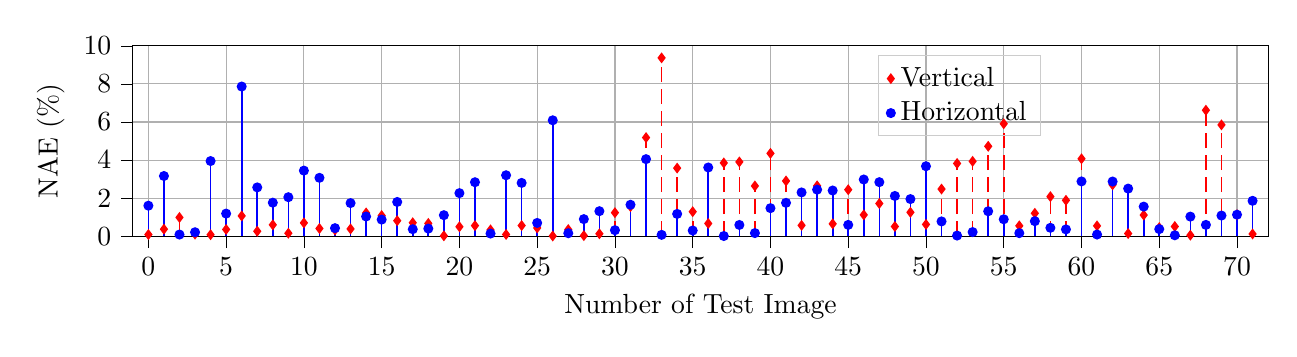
\begin{tikzpicture}

\definecolor{darkgray176}{RGB}{176,176,176}
\definecolor{lightgray204}{RGB}{204,204,204}

\begin{axis}[
width = 16cm,
height = 4cm,
legend cell align={left},
legend style={fill=none, text opacity=1, draw=lightgray204, at={(0.8,0.95)} },
tick align=outside,
tick pos=left,
x grid style={darkgray176},
xlabel={Number of Test Image},
xmajorgrids,
xmin=-1, xmax=72,
xtick style={color=black},
y grid style={darkgray176},
ylabel={NAE (\%)},
ymajorgrids,
ymin=0, ymax=10,
ytick style={color=black}
]
\path [draw=red, semithick, dash pattern=on 5.55pt off 2.4pt]
(axis cs:0,0)
--(axis cs:0,0.0891372893177833);

\path [draw=red, semithick, dash pattern=on 5.55pt off 2.4pt]
(axis cs:1,0)
--(axis cs:1,0.370584604455035);

\path [draw=red, semithick, dash pattern=on 5.55pt off 2.4pt]
(axis cs:2,0)
--(axis cs:2,0.986032709471848);

\path [draw=red, semithick, dash pattern=on 5.55pt off 2.4pt]
(axis cs:3,0)
--(axis cs:3,0.109907766079546);

\path [draw=red, semithick, dash pattern=on 5.55pt off 2.4pt]
(axis cs:4,0)
--(axis cs:4,0.0822666596545819);

\path [draw=red, semithick, dash pattern=on 5.55pt off 2.4pt]
(axis cs:5,0)
--(axis cs:5,0.357321088428495);

\path [draw=red, semithick, dash pattern=on 5.55pt off 2.4pt]
(axis cs:6,0)
--(axis cs:6,1.0675179989252);

\path [draw=red, semithick, dash pattern=on 5.55pt off 2.4pt]
(axis cs:7,0)
--(axis cs:7,0.26087508855736);

\path [draw=red, semithick, dash pattern=on 5.55pt off 2.4pt]
(axis cs:8,0)
--(axis cs:8,0.599942897007989);

\path [draw=red, semithick, dash pattern=on 5.55pt off 2.4pt]
(axis cs:9,0)
--(axis cs:9,0.157795275627521);

\path [draw=red, semithick, dash pattern=on 5.55pt off 2.4pt]
(axis cs:10,0)
--(axis cs:10,0.702147162506958);

\path [draw=red, semithick, dash pattern=on 5.55pt off 2.4pt]
(axis cs:11,0)
--(axis cs:11,0.406909215796071);

\path [draw=red, semithick, dash pattern=on 5.55pt off 2.4pt]
(axis cs:12,0)
--(axis cs:12,0.331458806193995);

\path [draw=red, semithick, dash pattern=on 5.55pt off 2.4pt]
(axis cs:13,0)
--(axis cs:13,0.383915047035242);

\path [draw=red, semithick, dash pattern=on 5.55pt off 2.4pt]
(axis cs:14,0)
--(axis cs:14,1.22389293172749);

\path [draw=red, semithick, dash pattern=on 5.55pt off 2.4pt]
(axis cs:15,0)
--(axis cs:15,1.08618673878954);

\path [draw=red, semithick, dash pattern=on 5.55pt off 2.4pt]
(axis cs:16,0)
--(axis cs:16,0.817461271972514);

\path [draw=red, semithick, dash pattern=on 5.55pt off 2.4pt]
(axis cs:17,0)
--(axis cs:17,0.708983367636591);

\path [draw=red, semithick, dash pattern=on 5.55pt off 2.4pt]
(axis cs:18,0)
--(axis cs:18,0.674357282147208);

\path [draw=red, semithick, dash pattern=on 5.55pt off 2.4pt]
(axis cs:19,0)
--(axis cs:19,0.0228714579279005);

\path [draw=red, semithick, dash pattern=on 5.55pt off 2.4pt]
(axis cs:20,0)
--(axis cs:20,0.497540760406243);

\path [draw=red, semithick, dash pattern=on 5.55pt off 2.4pt]
(axis cs:21,0)
--(axis cs:21,0.557443349354307);

\path [draw=red, semithick, dash pattern=on 5.55pt off 2.4pt]
(axis cs:22,0)
--(axis cs:22,0.33349683417564);

\path [draw=red, semithick, dash pattern=on 5.55pt off 2.4pt]
(axis cs:23,0)
--(axis cs:23,0.0933148019058486);

\path [draw=red, semithick, dash pattern=on 5.55pt off 2.4pt]
(axis cs:24,0)
--(axis cs:24,0.561745742877895);

\path [draw=red, semithick, dash pattern=on 5.55pt off 2.4pt]
(axis cs:25,0)
--(axis cs:25,0.435179364185227);

\path [draw=red, semithick, dash pattern=on 5.55pt off 2.4pt]
(axis cs:26,0)
--(axis cs:26,0.0115060568569611);

\path [draw=red, semithick, dash pattern=on 5.55pt off 2.4pt]
(axis cs:27,0)
--(axis cs:27,0.353191168275281);

\path [draw=red, semithick, dash pattern=on 5.55pt off 2.4pt]
(axis cs:28,0)
--(axis cs:28,0.03307448084071);

\path [draw=red, semithick, dash pattern=on 5.55pt off 2.4pt]
(axis cs:29,0)
--(axis cs:29,0.128556121680998);

\path [draw=red, semithick, dash pattern=on 5.55pt off 2.4pt]
(axis cs:30,0)
--(axis cs:30,1.23797858204359);

\path [draw=red, semithick, dash pattern=on 5.55pt off 2.4pt]
(axis cs:31,0)
--(axis cs:31,1.55669577142518);

\path [draw=red, semithick, dash pattern=on 5.55pt off 2.4pt]
(axis cs:32,0)
--(axis cs:32,5.18087173679666);

\path [draw=red, semithick, dash pattern=on 5.55pt off 2.4pt]
(axis cs:33,0)
--(axis cs:33,9.36596359845506);

\path [draw=red, semithick, dash pattern=on 5.55pt off 2.4pt]
(axis cs:34,0)
--(axis cs:34,3.57877826385229);

\path [draw=red, semithick, dash pattern=on 5.55pt off 2.4pt]
(axis cs:35,0)
--(axis cs:35,1.28796097434612);

\path [draw=red, semithick, dash pattern=on 5.55pt off 2.4pt]
(axis cs:36,0)
--(axis cs:36,0.670376647450484);

\path [draw=red, semithick, dash pattern=on 5.55pt off 2.4pt]
(axis cs:37,0)
--(axis cs:37,3.849417073192);

\path [draw=red, semithick, dash pattern=on 5.55pt off 2.4pt]
(axis cs:38,0)
--(axis cs:38,3.90441689015446);

\path [draw=red, semithick, dash pattern=on 5.55pt off 2.4pt]
(axis cs:39,0)
--(axis cs:39,2.64135164715969);

\path [draw=red, semithick, dash pattern=on 5.55pt off 2.4pt]
(axis cs:40,0)
--(axis cs:40,4.35127206115533);

\path [draw=red, semithick, dash pattern=on 5.55pt off 2.4pt]
(axis cs:41,0)
--(axis cs:41,2.90353625220088);

\path [draw=red, semithick, dash pattern=on 5.55pt off 2.4pt]
(axis cs:42,0)
--(axis cs:42,0.57060967755702);

\path [draw=red, semithick, dash pattern=on 5.55pt off 2.4pt]
(axis cs:43,0)
--(axis cs:43,2.64672702718658);

\path [draw=red, semithick, dash pattern=on 5.55pt off 2.4pt]
(axis cs:44,0)
--(axis cs:44,0.652177730307519);

\path [draw=red, semithick, dash pattern=on 5.55pt off 2.4pt]
(axis cs:45,0)
--(axis cs:45,2.44257111815915);

\path [draw=red, semithick, dash pattern=on 5.55pt off 2.4pt]
(axis cs:46,0)
--(axis cs:46,1.1222012979615);

\path [draw=red, semithick, dash pattern=on 5.55pt off 2.4pt]
(axis cs:47,0)
--(axis cs:47,1.7182354098259);

\path [draw=red, semithick, dash pattern=on 5.55pt off 2.4pt]
(axis cs:48,0)
--(axis cs:48,0.510461785691346);

\path [draw=red, semithick, dash pattern=on 5.55pt off 2.4pt]
(axis cs:49,0)
--(axis cs:49,1.25633791423234);

\path [draw=red, semithick, dash pattern=on 5.55pt off 2.4pt]
(axis cs:50,0)
--(axis cs:50,0.621333507441592);

\path [draw=red, semithick, dash pattern=on 5.55pt off 2.4pt]
(axis cs:51,0)
--(axis cs:51,2.47832255794163);

\path [draw=red, semithick, dash pattern=on 5.55pt off 2.4pt]
(axis cs:52,0)
--(axis cs:52,3.82364348447404);

\path [draw=red, semithick, dash pattern=on 5.55pt off 2.4pt]
(axis cs:53,0)
--(axis cs:53,3.93376682815643);

\path [draw=red, semithick, dash pattern=on 5.55pt off 2.4pt]
(axis cs:54,0)
--(axis cs:54,4.72364348422319);

\path [draw=red, semithick, dash pattern=on 5.55pt off 2.4pt]
(axis cs:55,0)
--(axis cs:55,5.90572014967425);

\path [draw=red, semithick, dash pattern=on 5.55pt off 2.4pt]
(axis cs:56,0)
--(axis cs:56,0.545846235128202);

\path [draw=red, semithick, dash pattern=on 5.55pt off 2.4pt]
(axis cs:57,0)
--(axis cs:57,1.20550889099103);

\path [draw=red, semithick, dash pattern=on 5.55pt off 2.4pt]
(axis cs:58,0)
--(axis cs:58,2.0798141224854);

\path [draw=red, semithick, dash pattern=on 5.55pt off 2.4pt]
(axis cs:59,0)
--(axis cs:59,1.88769559832437);

\path [draw=red, semithick, dash pattern=on 5.55pt off 2.4pt]
(axis cs:60,0)
--(axis cs:60,4.06760766382771);

\path [draw=red, semithick, dash pattern=on 5.55pt off 2.4pt]
(axis cs:61,0)
--(axis cs:61,0.544880396955417);

\path [draw=red, semithick, dash pattern=on 5.55pt off 2.4pt]
(axis cs:62,0)
--(axis cs:62,2.70220218089618);

\path [draw=red, semithick, dash pattern=on 5.55pt off 2.4pt]
(axis cs:63,0)
--(axis cs:63,0.142450855369382);

\path [draw=red, semithick, dash pattern=on 5.55pt off 2.4pt]
(axis cs:64,0)
--(axis cs:64,1.11221061384018);

\path [draw=red, semithick, dash pattern=on 5.55pt off 2.4pt]
(axis cs:65,0)
--(axis cs:65,0.455836859781922);

\path [draw=red, semithick, dash pattern=on 5.55pt off 2.4pt]
(axis cs:66,0)
--(axis cs:66,0.512493203062239);

\path [draw=red, semithick, dash pattern=on 5.55pt off 2.4pt]
(axis cs:67,0)
--(axis cs:67,0.0541307805128674);

\path [draw=red, semithick, dash pattern=on 5.55pt off 2.4pt]
(axis cs:68,0)
--(axis cs:68,6.61802465938199);

\path [draw=red, semithick, dash pattern=on 5.55pt off 2.4pt]
(axis cs:69,0)
--(axis cs:69,5.84877015002152);

\path [draw=red, semithick, dash pattern=on 5.55pt off 2.4pt]
(axis cs:70,0)
--(axis cs:70,1.13183003764784);

\path [draw=red, semithick, dash pattern=on 5.55pt off 2.4pt]
(axis cs:71,0)
--(axis cs:71,0.120663657892921);

\path [draw=blue, semithick]
(axis cs:0,0)
--(axis cs:0,1.60482432359047);

\path [draw=blue, semithick]
(axis cs:1,0)
--(axis cs:1,3.16337308379479);

\path [draw=blue, semithick]
(axis cs:2,0)
--(axis cs:2,0.088518954929298);

\path [draw=blue, semithick]
(axis cs:3,0)
--(axis cs:3,0.209946522328121);

\path [draw=blue, semithick]
(axis cs:4,0)
--(axis cs:4,3.94868101726816);

\path [draw=blue, semithick]
(axis cs:5,0)
--(axis cs:5,1.1890567311829);

\path [draw=blue, semithick]
(axis cs:6,0)
--(axis cs:6,7.86157482848479);

\path [draw=blue, semithick]
(axis cs:7,0)
--(axis cs:7,2.56533097803157);

\path [draw=blue, semithick]
(axis cs:8,0)
--(axis cs:8,1.76323691381998);

\path [draw=blue, semithick]
(axis cs:9,0)
--(axis cs:9,2.05101657514193);

\path [draw=blue, semithick]
(axis cs:10,0)
--(axis cs:10,3.44695063169501);

\path [draw=blue, semithick]
(axis cs:11,0)
--(axis cs:11,3.06769932233839);

\path [draw=blue, semithick]
(axis cs:12,0)
--(axis cs:12,0.425124444156019);

\path [draw=blue, semithick]
(axis cs:13,0)
--(axis cs:13,1.74108652685822);

\path [draw=blue, semithick]
(axis cs:14,0)
--(axis cs:14,1.03592652805637);

\path [draw=blue, semithick]
(axis cs:15,0)
--(axis cs:15,0.874851553696532);

\path [draw=blue, semithick]
(axis cs:16,0)
--(axis cs:16,1.80032370895501);

\path [draw=blue, semithick]
(axis cs:17,0)
--(axis cs:17,0.369830616734339);

\path [draw=blue, semithick]
(axis cs:18,0)
--(axis cs:18,0.401111073332179);

\path [draw=blue, semithick]
(axis cs:19,0)
--(axis cs:19,1.10642535423046);

\path [draw=blue, semithick]
(axis cs:20,0)
--(axis cs:20,2.26387154762841);

\path [draw=blue, semithick]
(axis cs:21,0)
--(axis cs:21,2.83718646720633);

\path [draw=blue, semithick]
(axis cs:22,0)
--(axis cs:22,0.1406937077281);

\path [draw=blue, semithick]
(axis cs:23,0)
--(axis cs:23,3.20267812839011);

\path [draw=blue, semithick]
(axis cs:24,0)
--(axis cs:24,2.80031096883609);

\path [draw=blue, semithick]
(axis cs:25,0)
--(axis cs:25,0.699085408205588);

\path [draw=blue, semithick]
(axis cs:26,0)
--(axis cs:26,6.08843810697338);

\path [draw=blue, semithick]
(axis cs:27,0)
--(axis cs:27,0.15864254759884);

\path [draw=blue, semithick]
(axis cs:28,0)
--(axis cs:28,0.89939964672912);

\path [draw=blue, semithick]
(axis cs:29,0)
--(axis cs:29,1.31660840779235);

\path [draw=blue, semithick]
(axis cs:30,0)
--(axis cs:30,0.318010242119301);

\path [draw=blue, semithick]
(axis cs:31,0)
--(axis cs:31,1.65439344125001);

\path [draw=blue, semithick]
(axis cs:32,0)
--(axis cs:32,4.0483540218392);

\path [draw=blue, semithick]
(axis cs:33,0)
--(axis cs:33,0.0730891529074287);

\path [draw=blue, semithick]
(axis cs:34,0)
--(axis cs:34,1.17231958118489);

\path [draw=blue, semithick]
(axis cs:35,0)
--(axis cs:35,0.300970256518251);

\path [draw=blue, semithick]
(axis cs:36,0)
--(axis cs:36,3.61055197209082);

\path [draw=blue, semithick]
(axis cs:37,0)
--(axis cs:37,0.012149964675335);

\path [draw=blue, semithick]
(axis cs:38,0)
--(axis cs:38,0.592998250688215);

\path [draw=blue, semithick]
(axis cs:39,0)
--(axis cs:39,0.164741687083903);

\path [draw=blue, semithick]
(axis cs:40,0)
--(axis cs:40,1.47468837822852);

\path [draw=blue, semithick]
(axis cs:41,0)
--(axis cs:41,1.75416009928301);

\path [draw=blue, semithick]
(axis cs:42,0)
--(axis cs:42,2.30136441803097);

\path [draw=blue, semithick]
(axis cs:43,0)
--(axis cs:43,2.44754392202821);

\path [draw=blue, semithick]
(axis cs:44,0)
--(axis cs:44,2.40126263823437);

\path [draw=blue, semithick]
(axis cs:45,0)
--(axis cs:45,0.596231763375445);

\path [draw=blue, semithick]
(axis cs:46,0)
--(axis cs:46,2.97974726299161);

\path [draw=blue, semithick]
(axis cs:47,0)
--(axis cs:47,2.8403540068345);

\path [draw=blue, semithick]
(axis cs:48,0)
--(axis cs:48,2.11609785007945);

\path [draw=blue, semithick]
(axis cs:49,0)
--(axis cs:49,1.95178155012636);

\path [draw=blue, semithick]
(axis cs:50,0)
--(axis cs:50,3.67679795630587);

\path [draw=blue, semithick]
(axis cs:51,0)
--(axis cs:51,0.778316601196557);

\path [draw=blue, semithick]
(axis cs:52,0)
--(axis cs:52,0.0354201830380699);

\path [draw=blue, semithick]
(axis cs:53,0)
--(axis cs:53,0.219323231101386);

\path [draw=blue, semithick]
(axis cs:54,0)
--(axis cs:54,1.31106498447003);

\path [draw=blue, semithick]
(axis cs:55,0)
--(axis cs:55,0.891170629365694);

\path [draw=blue, semithick]
(axis cs:56,0)
--(axis cs:56,0.162700341116095);

\path [draw=blue, semithick]
(axis cs:57,0)
--(axis cs:57,0.791304910412589);

\path [draw=blue, semithick]
(axis cs:58,0)
--(axis cs:58,0.442745412109532);

\path [draw=blue, semithick]
(axis cs:59,0)
--(axis cs:59,0.359649677668585);

\path [draw=blue, semithick]
(axis cs:60,0)
--(axis cs:60,2.87901485242971);

\path [draw=blue, semithick]
(axis cs:61,0)
--(axis cs:61,0.0890789423451848);

\path [draw=blue, semithick]
(axis cs:62,0)
--(axis cs:62,2.87360305730203);

\path [draw=blue, semithick]
(axis cs:63,0)
--(axis cs:63,2.50185328732075);

\path [draw=blue, semithick]
(axis cs:64,0)
--(axis cs:64,1.55591787676345);

\path [draw=blue, semithick]
(axis cs:65,0)
--(axis cs:65,0.373843770605919);

\path [draw=blue, semithick]
(axis cs:66,0)
--(axis cs:66,0.0500395673834782);

\path [draw=blue, semithick]
(axis cs:67,0)
--(axis cs:67,1.03094775175834);

\path [draw=blue, semithick]
(axis cs:68,0)
--(axis cs:68,0.596176262631349);

\path [draw=blue, semithick]
(axis cs:69,0)
--(axis cs:69,1.08649993637958);

\path [draw=blue, semithick]
(axis cs:70,0)
--(axis cs:70,1.13183586227048);

\path [draw=blue, semithick]
(axis cs:71,0)
--(axis cs:71,1.86047529565208);

\addplot [semithick, red, mark=diamond*, mark size=1.5, mark options={solid}, only marks]
table {%
0 0.0891372893177833
1 0.370584604455035
2 0.986032709471848
3 0.109907766079546
4 0.0822666596545819
5 0.357321088428495
6 1.0675179989252
7 0.26087508855736
8 0.599942897007989
9 0.157795275627521
10 0.702147162506958
11 0.406909215796071
12 0.331458806193995
13 0.383915047035242
14 1.22389293172749
15 1.08618673878954
16 0.817461271972514
17 0.708983367636591
18 0.674357282147208
19 0.0228714579279005
20 0.497540760406243
21 0.557443349354307
22 0.33349683417564
23 0.0933148019058486
24 0.561745742877895
25 0.435179364185227
26 0.0115060568569611
27 0.353191168275281
28 0.03307448084071
29 0.128556121680998
30 1.23797858204359
31 1.55669577142518
32 5.18087173679666
33 9.36596359845506
34 3.57877826385229
35 1.28796097434612
36 0.670376647450484
37 3.849417073192
38 3.90441689015446
39 2.64135164715969
40 4.35127206115533
41 2.90353625220088
42 0.57060967755702
43 2.64672702718658
44 0.652177730307519
45 2.44257111815915
46 1.1222012979615
47 1.7182354098259
48 0.510461785691346
49 1.25633791423234
50 0.621333507441592
51 2.47832255794163
52 3.82364348447404
53 3.93376682815643
54 4.72364348422319
55 5.90572014967425
56 0.545846235128202
57 1.20550889099103
58 2.0798141224854
59 1.88769559832437
60 4.06760766382771
61 0.544880396955417
62 2.70220218089618
63 0.142450855369382
64 1.11221061384018
65 0.455836859781922
66 0.512493203062239
67 0.0541307805128674
68 6.61802465938199
69 5.84877015002152
70 1.13183003764784
71 0.120663657892921
};\addlegendentry{Vertical}
\addplot [semithick, blue, mark=*, mark size=1.5, mark options={solid}, only marks]
table {%
0 1.60482432359047
1 3.16337308379479
2 0.088518954929298
3 0.209946522328121
4 3.94868101726816
5 1.1890567311829
6 7.86157482848479
7 2.56533097803157
8 1.76323691381998
9 2.05101657514193
10 3.44695063169501
11 3.06769932233839
12 0.425124444156019
13 1.74108652685822
14 1.03592652805637
15 0.874851553696532
16 1.80032370895501
17 0.369830616734339
18 0.401111073332179
19 1.10642535423046
20 2.26387154762841
21 2.83718646720633
22 0.1406937077281
23 3.20267812839011
24 2.80031096883609
25 0.699085408205588
26 6.08843810697338
27 0.15864254759884
28 0.89939964672912
29 1.31660840779235
30 0.318010242119301
31 1.65439344125001
32 4.0483540218392
33 0.0730891529074287
34 1.17231958118489
35 0.300970256518251
36 3.61055197209082
37 0.012149964675335
38 0.592998250688215
39 0.164741687083903
40 1.47468837822852
41 1.75416009928301
42 2.30136441803097
43 2.44754392202821
44 2.40126263823437
45 0.596231763375445
46 2.97974726299161
47 2.8403540068345
48 2.11609785007945
49 1.95178155012636
50 3.67679795630587
51 0.778316601196557
52 0.0354201830380699
53 0.219323231101386
54 1.31106498447003
55 0.891170629365694
56 0.162700341116095
57 0.791304910412589
58 0.442745412109532
59 0.359649677668585
60 2.87901485242971
61 0.0890789423451848
62 2.87360305730203
63 2.50185328732075
64 1.55591787676345
65 0.373843770605919
66 0.0500395673834782
67 1.03094775175834
68 0.596176262631349
69 1.08649993637958
70 1.13183586227048
71 1.86047529565208
};\addlegendentry{Horizontal}
\end{axis}

\end{tikzpicture}
\\
 (c) \\ 
 % This file was created with tikzplotlib v0.10.1.
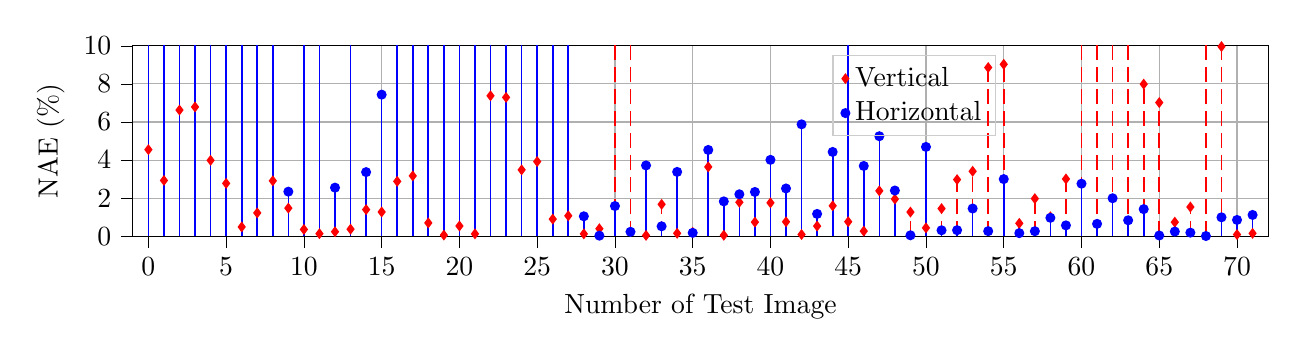
\begin{tikzpicture}

\definecolor{darkgray176}{RGB}{176,176,176}
\definecolor{lightgray204}{RGB}{204,204,204}

\begin{axis}[
width = 16cm,
height = 4cm,
legend cell align={left},
legend style={fill = none, text opacity=1, draw=lightgray204, at={(0.76,0.95)} },
tick align=outside,
tick pos=left,
x grid style={darkgray176},
xlabel={Number of Test Image},
xmajorgrids,
xmin=-1, xmax=72,
xtick style={color=black},
y grid style={darkgray176},
ylabel={NAE (\%)},
ymajorgrids,
ymin=0, ymax=10,
ytick style={color=black}
]
\path [draw=red, semithick, dash pattern=on 5.55pt off 2.4pt]
(axis cs:0,0)
--(axis cs:0,4.5483855778803);

\path [draw=red, semithick, dash pattern=on 5.55pt off 2.4pt]
(axis cs:1,0)
--(axis cs:1,2.9292841952533);

\path [draw=red, semithick, dash pattern=on 5.55pt off 2.4pt]
(axis cs:2,0)
--(axis cs:2,6.62645610841829);

\path [draw=red, semithick, dash pattern=on 5.55pt off 2.4pt]
(axis cs:3,0)
--(axis cs:3,6.78846952332171);

\path [draw=red, semithick, dash pattern=on 5.55pt off 2.4pt]
(axis cs:4,0)
--(axis cs:4,3.98599574299314);

\path [draw=red, semithick, dash pattern=on 5.55pt off 2.4pt]
(axis cs:5,0)
--(axis cs:5,2.7756684893379);

\path [draw=red, semithick, dash pattern=on 5.55pt off 2.4pt]
(axis cs:6,0)
--(axis cs:6,0.488267940090136);

\path [draw=red, semithick, dash pattern=on 5.55pt off 2.4pt]
(axis cs:7,0)
--(axis cs:7,1.22326551734608);

\path [draw=red, semithick, dash pattern=on 5.55pt off 2.4pt]
(axis cs:8,0)
--(axis cs:8,2.90977868853943);

\path [draw=red, semithick, dash pattern=on 5.55pt off 2.4pt]
(axis cs:9,0)
--(axis cs:9,1.47605435428485);

\path [draw=red, semithick, dash pattern=on 5.55pt off 2.4pt]
(axis cs:10,0)
--(axis cs:10,0.354545808613438);

\path [draw=red, semithick, dash pattern=on 5.55pt off 2.4pt]
(axis cs:11,0)
--(axis cs:11,0.134605226059808);

\path [draw=red, semithick, dash pattern=on 5.55pt off 2.4pt]
(axis cs:12,0)
--(axis cs:12,0.237049598001875);

\path [draw=red, semithick, dash pattern=on 5.55pt off 2.4pt]
(axis cs:13,0)
--(axis cs:13,0.37250971966461);

\path [draw=red, semithick, dash pattern=on 5.55pt off 2.4pt]
(axis cs:14,0)
--(axis cs:14,1.40024444895354);

\path [draw=red, semithick, dash pattern=on 5.55pt off 2.4pt]
(axis cs:15,0)
--(axis cs:15,1.27429629808493);

\path [draw=red, semithick, dash pattern=on 5.55pt off 2.4pt]
(axis cs:16,0)
--(axis cs:16,2.88289168100941);

\path [draw=red, semithick, dash pattern=on 5.55pt off 2.4pt]
(axis cs:17,0)
--(axis cs:17,3.1686077537258);

\path [draw=red, semithick, dash pattern=on 5.55pt off 2.4pt]
(axis cs:18,0)
--(axis cs:18,0.699726065157247);

\path [draw=red, semithick, dash pattern=on 5.55pt off 2.4pt]
(axis cs:19,0)
--(axis cs:19,0.0589048045037918);

\path [draw=red, semithick, dash pattern=on 5.55pt off 2.4pt]
(axis cs:20,0)
--(axis cs:20,0.538795448616386);

\path [draw=red, semithick, dash pattern=on 5.55pt off 2.4pt]
(axis cs:21,0)
--(axis cs:21,0.123797425539182);

\path [draw=red, semithick, dash pattern=on 5.55pt off 2.4pt]
(axis cs:22,0)
--(axis cs:22,7.37726584973173);

\path [draw=red, semithick, dash pattern=on 5.55pt off 2.4pt]
(axis cs:23,0)
--(axis cs:23,7.29103705633353);

\path [draw=red, semithick, dash pattern=on 5.55pt off 2.4pt]
(axis cs:24,0)
--(axis cs:24,3.48592496172199);

\path [draw=red, semithick, dash pattern=on 5.55pt off 2.4pt]
(axis cs:25,0)
--(axis cs:25,3.92071541688619);

\path [draw=red, semithick, dash pattern=on 5.55pt off 2.4pt]
(axis cs:26,0)
--(axis cs:26,0.901441044251731);

\path [draw=red, semithick, dash pattern=on 5.55pt off 2.4pt]
(axis cs:27,0)
--(axis cs:27,1.07347984999687);

\path [draw=red, semithick, dash pattern=on 5.55pt off 2.4pt]
(axis cs:28,0)
--(axis cs:28,0.125353601553148);

\path [draw=red, semithick, dash pattern=on 5.55pt off 2.4pt]
(axis cs:29,0)
--(axis cs:29,0.393938547036884);

\path [draw=red, semithick, dash pattern=on 5.55pt off 2.4pt]
(axis cs:30,0)
--(axis cs:30,16.3856469028772);

\path [draw=red, semithick, dash pattern=on 5.55pt off 2.4pt]
(axis cs:31,0)
--(axis cs:31,15.7549969136119);

\path [draw=red, semithick, dash pattern=on 5.55pt off 2.4pt]
(axis cs:32,0)
--(axis cs:32,0.0449959270112771);

\path [draw=red, semithick, dash pattern=on 5.55pt off 2.4pt]
(axis cs:33,0)
--(axis cs:33,1.67536462034163);

\path [draw=red, semithick, dash pattern=on 5.55pt off 2.4pt]
(axis cs:34,0)
--(axis cs:34,0.155591449976825);

\path [draw=red, semithick, dash pattern=on 5.55pt off 2.4pt]
(axis cs:35,0)
--(axis cs:35,0.20494097953652);

\path [draw=red, semithick, dash pattern=on 5.55pt off 2.4pt]
(axis cs:36,0)
--(axis cs:36,3.64091876176312);

\path [draw=red, semithick, dash pattern=on 5.55pt off 2.4pt]
(axis cs:37,0)
--(axis cs:37,0.0531733233889002);

\path [draw=red, semithick, dash pattern=on 5.55pt off 2.4pt]
(axis cs:38,0)
--(axis cs:38,1.78579310350601);

\path [draw=red, semithick, dash pattern=on 5.55pt off 2.4pt]
(axis cs:39,0)
--(axis cs:39,0.741461245187437);

\path [draw=red, semithick, dash pattern=on 5.55pt off 2.4pt]
(axis cs:40,0)
--(axis cs:40,1.75490185989792);

\path [draw=red, semithick, dash pattern=on 5.55pt off 2.4pt]
(axis cs:41,0)
--(axis cs:41,0.758780750766022);

\path [draw=red, semithick, dash pattern=on 5.55pt off 2.4pt]
(axis cs:42,0)
--(axis cs:42,0.0908473475848361);

\path [draw=red, semithick, dash pattern=on 5.55pt off 2.4pt]
(axis cs:43,0)
--(axis cs:43,0.533508658700943);

\path [draw=red, semithick, dash pattern=on 5.55pt off 2.4pt]
(axis cs:44,0)
--(axis cs:44,1.59827014928415);

\path [draw=red, semithick, dash pattern=on 5.55pt off 2.4pt]
(axis cs:45,0)
--(axis cs:45,0.763055523457512);

\path [draw=red, semithick, dash pattern=on 5.55pt off 2.4pt]
(axis cs:46,0)
--(axis cs:46,0.26966330839801);

\path [draw=red, semithick, dash pattern=on 5.55pt off 2.4pt]
(axis cs:47,0)
--(axis cs:47,2.38366360084578);

\path [draw=red, semithick, dash pattern=on 5.55pt off 2.4pt]
(axis cs:48,0)
--(axis cs:48,1.95304707057154);

\path [draw=red, semithick, dash pattern=on 5.55pt off 2.4pt]
(axis cs:49,0)
--(axis cs:49,1.27030903324055);

\path [draw=red, semithick, dash pattern=on 5.55pt off 2.4pt]
(axis cs:50,0)
--(axis cs:50,0.439691288626266);

\path [draw=red, semithick, dash pattern=on 5.55pt off 2.4pt]
(axis cs:51,0)
--(axis cs:51,1.45248753658255);

\path [draw=red, semithick, dash pattern=on 5.55pt off 2.4pt]
(axis cs:52,0)
--(axis cs:52,2.97509646249189);

\path [draw=red, semithick, dash pattern=on 5.55pt off 2.4pt]
(axis cs:53,0)
--(axis cs:53,3.41124622266625);

\path [draw=red, semithick, dash pattern=on 5.55pt off 2.4pt]
(axis cs:54,0)
--(axis cs:54,8.85965415721278);

\path [draw=red, semithick, dash pattern=on 5.55pt off 2.4pt]
(axis cs:55,0)
--(axis cs:55,9.02927407011405);

\path [draw=red, semithick, dash pattern=on 5.55pt off 2.4pt]
(axis cs:56,0)
--(axis cs:56,0.678797291054475);

\path [draw=red, semithick, dash pattern=on 5.55pt off 2.4pt]
(axis cs:57,0)
--(axis cs:57,1.97423007135386);

\path [draw=red, semithick, dash pattern=on 5.55pt off 2.4pt]
(axis cs:58,0)
--(axis cs:58,1.02040273324581);

\path [draw=red, semithick, dash pattern=on 5.55pt off 2.4pt]
(axis cs:59,0)
--(axis cs:59,3.00850660901738);

\path [draw=red, semithick, dash pattern=on 5.55pt off 2.4pt]
(axis cs:60,0)
--(axis cs:60,11.9451262295872);

\path [draw=red, semithick, dash pattern=on 5.55pt off 2.4pt]
(axis cs:61,0)
--(axis cs:61,10.2315992248775);

\path [draw=red, semithick, dash pattern=on 5.55pt off 2.4pt]
(axis cs:62,0)
--(axis cs:62,15.9657332616532);

\path [draw=red, semithick, dash pattern=on 5.55pt off 2.4pt]
(axis cs:63,0)
--(axis cs:63,15.690493006004);

\path [draw=red, semithick, dash pattern=on 5.55pt off 2.4pt]
(axis cs:64,0)
--(axis cs:64,7.98802207698468);

\path [draw=red, semithick, dash pattern=on 5.55pt off 2.4pt]
(axis cs:65,0)
--(axis cs:65,7.01930008480202);

\path [draw=red, semithick, dash pattern=on 5.55pt off 2.4pt]
(axis cs:66,0)
--(axis cs:66,0.738308660227799);

\path [draw=red, semithick, dash pattern=on 5.55pt off 2.4pt]
(axis cs:67,0)
--(axis cs:67,1.53603643496194);

\path [draw=red, semithick, dash pattern=on 5.55pt off 2.4pt]
(axis cs:68,0)
--(axis cs:68,10.9257540655324);

\path [draw=red, semithick, dash pattern=on 5.55pt off 2.4pt]
(axis cs:69,0)
--(axis cs:69,9.96019052786003);

\path [draw=red, semithick, dash pattern=on 5.55pt off 2.4pt]
(axis cs:70,0)
--(axis cs:70,0.0886150983026949);

\path [draw=red, semithick, dash pattern=on 5.55pt off 2.4pt]
(axis cs:71,0)
--(axis cs:71,0.151611007057893);

\path [draw=blue, semithick]
(axis cs:0,0)
--(axis cs:0,30.2414812882555);

\path [draw=blue, semithick]
(axis cs:1,0)
--(axis cs:1,27.95806113769);

\path [draw=blue, semithick]
(axis cs:2,0)
--(axis cs:2,30.6613927972566);

\path [draw=blue, semithick]
(axis cs:3,0)
--(axis cs:3,27.4218542058029);

\path [draw=blue, semithick]
(axis cs:4,0)
--(axis cs:4,19.307446450645);

\path [draw=blue, semithick]
(axis cs:5,0)
--(axis cs:5,25.095098033072);

\path [draw=blue, semithick]
(axis cs:6,0)
--(axis cs:6,19.5529693220895);

\path [draw=blue, semithick]
(axis cs:7,0)
--(axis cs:7,25.3873647377601);

\path [draw=blue, semithick]
(axis cs:8,0)
--(axis cs:8,41.0315376832457);

\path [draw=blue, semithick]
(axis cs:9,0)
--(axis cs:9,2.34060997441059);

\path [draw=blue, semithick]
(axis cs:10,0)
--(axis cs:10,40.0360435774602);

\path [draw=blue, semithick]
(axis cs:11,0)
--(axis cs:11,48.1905710669052);

\path [draw=blue, semithick]
(axis cs:12,0)
--(axis cs:12,2.55179154810946);

\path [draw=blue, semithick]
(axis cs:13,0)
--(axis cs:13,32.3854709740873);

\path [draw=blue, semithick]
(axis cs:14,0)
--(axis cs:14,3.36739303648128);

\path [draw=blue, semithick]
(axis cs:15,0)
--(axis cs:15,7.43580640995085);

\path [draw=blue, semithick]
(axis cs:16,0)
--(axis cs:16,27.8213651918377);

\path [draw=blue, semithick]
(axis cs:17,0)
--(axis cs:17,21.2279278951991);

\path [draw=blue, semithick]
(axis cs:18,0)
--(axis cs:18,27.2047056862851);

\path [draw=blue, semithick]
(axis cs:19,0)
--(axis cs:19,37.5098150154223);

\path [draw=blue, semithick]
(axis cs:20,0)
--(axis cs:20,41.317895001);

\path [draw=blue, semithick]
(axis cs:21,0)
--(axis cs:21,27.1381487073405);

\path [draw=blue, semithick]
(axis cs:22,0)
--(axis cs:22,41.2032250998795);

\path [draw=blue, semithick]
(axis cs:23,0)
--(axis cs:23,18.0217421543486);

\path [draw=blue, semithick]
(axis cs:24,0)
--(axis cs:24,45.8029627337605);

\path [draw=blue, semithick]
(axis cs:25,0)
--(axis cs:25,23.6255899089801);

\path [draw=blue, semithick]
(axis cs:26,0)
--(axis cs:26,22.2074965804325);

\path [draw=blue, semithick]
(axis cs:27,0)
--(axis cs:27,24.3250551595227);

\path [draw=blue, semithick]
(axis cs:28,0)
--(axis cs:28,1.04766718441718);

\path [draw=blue, semithick]
(axis cs:29,0)
--(axis cs:29,0.0299385808005757);

\path [draw=blue, semithick]
(axis cs:30,0)
--(axis cs:30,1.58582006544605);

\path [draw=blue, semithick]
(axis cs:31,0)
--(axis cs:31,0.232735480523358);

\path [draw=blue, semithick]
(axis cs:32,0)
--(axis cs:32,3.71767887406965);

\path [draw=blue, semithick]
(axis cs:33,0)
--(axis cs:33,0.522090685520483);

\path [draw=blue, semithick]
(axis cs:34,0)
--(axis cs:34,3.37895812896285);

\path [draw=blue, semithick]
(axis cs:35,0)
--(axis cs:35,0.178018291878438);

\path [draw=blue, semithick]
(axis cs:36,0)
--(axis cs:36,4.53158248459313);

\path [draw=blue, semithick]
(axis cs:37,0)
--(axis cs:37,1.83103494684361);

\path [draw=blue, semithick]
(axis cs:38,0)
--(axis cs:38,2.20391734194135);

\path [draw=blue, semithick]
(axis cs:39,0)
--(axis cs:39,2.32556212206007);

\path [draw=blue, semithick]
(axis cs:40,0)
--(axis cs:40,4.01169918301993);

\path [draw=blue, semithick]
(axis cs:41,0)
--(axis cs:41,2.50822934109157);

\path [draw=blue, semithick]
(axis cs:42,0)
--(axis cs:42,5.87693944148154);

\path [draw=blue, semithick]
(axis cs:43,0)
--(axis cs:43,1.17299801026202);

\path [draw=blue, semithick]
(axis cs:44,0)
--(axis cs:44,4.42664107676901);

\path [draw=blue, semithick]
(axis cs:45,0)
--(axis cs:45,15.0125376360674);

\path [draw=blue, semithick]
(axis cs:46,0)
--(axis cs:46,3.69126854781521);

\path [draw=blue, semithick]
(axis cs:47,0)
--(axis cs:47,5.25279368577902);

\path [draw=blue, semithick]
(axis cs:48,0)
--(axis cs:48,2.40151533688411);

\path [draw=blue, semithick]
(axis cs:49,0)
--(axis cs:49,0.0496855520163309);

\path [draw=blue, semithick]
(axis cs:50,0)
--(axis cs:50,4.69094307473997);

\path [draw=blue, semithick]
(axis cs:51,0)
--(axis cs:51,0.312696381101893);

\path [draw=blue, semithick]
(axis cs:52,0)
--(axis cs:52,0.31771856851197);

\path [draw=blue, semithick]
(axis cs:53,0)
--(axis cs:53,1.45565195678528);

\path [draw=blue, semithick]
(axis cs:54,0)
--(axis cs:54,0.26724549795861);

\path [draw=blue, semithick]
(axis cs:55,0)
--(axis cs:55,3.00138582866817);

\path [draw=blue, semithick]
(axis cs:56,0)
--(axis cs:56,0.162624090916667);

\path [draw=blue, semithick]
(axis cs:57,0)
--(axis cs:57,0.264519820086909);

\path [draw=blue, semithick]
(axis cs:58,0)
--(axis cs:58,0.967417863345889);

\path [draw=blue, semithick]
(axis cs:59,0)
--(axis cs:59,0.570622885705173);

\path [draw=blue, semithick]
(axis cs:60,0)
--(axis cs:60,2.7597668324754);

\path [draw=blue, semithick]
(axis cs:61,0)
--(axis cs:61,0.65074453809283);

\path [draw=blue, semithick]
(axis cs:62,0)
--(axis cs:62,1.99494639541747);

\path [draw=blue, semithick]
(axis cs:63,0)
--(axis cs:63,0.837776926202928);

\path [draw=blue, semithick]
(axis cs:64,0)
--(axis cs:64,1.42330131937866);

\path [draw=blue, semithick]
(axis cs:65,0)
--(axis cs:65,0.039448729200628);

\path [draw=blue, semithick]
(axis cs:66,0)
--(axis cs:66,0.245897301052074);

\path [draw=blue, semithick]
(axis cs:67,0)
--(axis cs:67,0.18861139035031);

\path [draw=blue, semithick]
(axis cs:68,0)
--(axis cs:68,0.0115963535672206);

\path [draw=blue, semithick]
(axis cs:69,0)
--(axis cs:69,0.99403090057316);

\path [draw=blue, semithick]
(axis cs:70,0)
--(axis cs:70,0.857170867882865);

\path [draw=blue, semithick]
(axis cs:71,0)
--(axis cs:71,1.11871987627772);

\addplot [semithick, red, mark=diamond*, mark size=1.5, mark options={solid}, only marks]
table {%
0 4.5483855778803
1 2.9292841952533
2 6.62645610841829
3 6.78846952332171
4 3.98599574299314
5 2.7756684893379
6 0.488267940090136
7 1.22326551734608
8 2.90977868853943
9 1.47605435428485
10 0.354545808613438
11 0.134605226059808
12 0.237049598001875
13 0.37250971966461
14 1.40024444895354
15 1.27429629808493
16 2.88289168100941
17 3.1686077537258
18 0.699726065157247
19 0.0589048045037918
20 0.538795448616386
21 0.123797425539182
22 7.37726584973173
23 7.29103705633353
24 3.48592496172199
25 3.92071541688619
26 0.901441044251731
27 1.07347984999687
28 0.125353601553148
29 0.393938547036884
30 16.3856469028772
31 15.7549969136119
32 0.0449959270112771
33 1.67536462034163
34 0.155591449976825
35 0.20494097953652
36 3.64091876176312
37 0.0531733233889002
38 1.78579310350601
39 0.741461245187437
40 1.75490185989792
41 0.758780750766022
42 0.0908473475848361
43 0.533508658700943
44 1.59827014928415
45 0.763055523457512
46 0.26966330839801
47 2.38366360084578
48 1.95304707057154
49 1.27030903324055
50 0.439691288626266
51 1.45248753658255
52 2.97509646249189
53 3.41124622266625
54 8.85965415721278
55 9.02927407011405
56 0.678797291054475
57 1.97423007135386
58 1.02040273324581
59 3.00850660901738
60 11.9451262295872
61 10.2315992248775
62 15.9657332616532
63 15.690493006004
64 7.98802207698468
65 7.01930008480202
66 0.738308660227799
67 1.53603643496194
68 10.9257540655324
69 9.96019052786003
70 0.0886150983026949
71 0.151611007057893
};\addlegendentry{Vertical}
\addplot [semithick, blue, mark=*, mark size=1.5, mark options={solid}, only marks]
table {%
0 30.2414812882555
1 27.95806113769
2 30.6613927972566
3 27.4218542058029
4 19.307446450645
5 25.095098033072
6 19.5529693220895
7 25.3873647377601
8 41.0315376832457
9 2.34060997441059
10 40.0360435774602
11 48.1905710669052
12 2.55179154810946
13 32.3854709740873
14 3.36739303648128
15 7.43580640995085
16 27.8213651918377
17 21.2279278951991
18 27.2047056862851
19 37.5098150154223
20 41.317895001
21 27.1381487073405
22 41.2032250998795
23 18.0217421543486
24 45.8029627337605
25 23.6255899089801
26 22.2074965804325
27 24.3250551595227
28 1.04766718441718
29 0.0299385808005757
30 1.58582006544605
31 0.232735480523358
32 3.71767887406965
33 0.522090685520483
34 3.37895812896285
35 0.178018291878438
36 4.53158248459313
37 1.83103494684361
38 2.20391734194135
39 2.32556212206007
40 4.01169918301993
41 2.50822934109157
42 5.87693944148154
43 1.17299801026202
44 4.42664107676901
45 15.0125376360674
46 3.69126854781521
47 5.25279368577902
48 2.40151533688411
49 0.0496855520163309
50 4.69094307473997
51 0.312696381101893
52 0.31771856851197
53 1.45565195678528
54 0.26724549795861
55 3.00138582866817
56 0.162624090916667
57 0.264519820086909
58 0.967417863345889
59 0.570622885705173
60 2.7597668324754
61 0.65074453809283
62 1.99494639541747
63 0.837776926202928
64 1.42330131937866
65 0.039448729200628
66 0.245897301052074
67 0.18861139035031
68 0.0115963535672206
69 0.99403090057316
70 0.857170867882865
71 1.11871987627772
};\addlegendentry{Horizontal}
\end{axis}

\end{tikzpicture}

 \\
 (d) 
\end{tabular}
\caption{Vertical and horizontal thread density normalized absolute error (NAE) (\%) of every sample in the test dataset for (a) the best Reg model, (b) the Inc-Dice in \cite{Bejarano2023} and (c) the FT.} \label{fig:TestSamples}
\end{figure*}


\section{Canvas Analysis}\label{sec:exp}

In the following, we study a series of canvases. The X-ray plate image is first re-scaled to 200 pixels per cm, to get an image of size $r \times s$, the height by the width of the image in pixels, respectively. Then it is pre-processed. Patches of $1\times 1$ cm all over the canvas are the input to the regression DL. Depending on the spatial resolution needed for the threads maps, the patches can be overlapped from one patch to the next one by some pixels, $o$, either vertically or horizontally. Therefore, we will process $p\times q$ patches, where $p= \lfloor r\cdot (1-o)/200 \rfloor$ and $q=\lfloor s\cdot (1-o)/200 \rfloor$. In the SS algorithm, we set $F=40\cdot 200/(1-o)$ pixels, i.e., we process blocks of $40\times q$ patches. After processing the image we get two matrices with the estimated values for the vertical and horizontal thread densities. The matrices can be interpreted as images where the pixel value indexes a color, hereafter denoted by threads density maps. 
%
We compare threads density maps obtained with the new regression DL approach to the ones of other previous approaches as frequency analysis \cite{Simois18}, ATCA approach \cite{Maaten15} or segmentation DL \cite{Bejarano2023}. The color of any pixel of the color densities maps encodes the value of the thread density in thr/cm, estimated for the $1\times 1$ cm image area in that location, except for the  ATCA \cite{Maaten15} that computes densities from crossing points at that position.


\subsection{Semi-Supervised analysis with Ixion by Ribera}
The most used method for frequency analysis is FT, where no labeling is needed. If the fabric presents quite a uniform pattern where both weft and warp are clearly observed, the FT provides a quite good estimation of the thread densities. The painting Ixion by Ribera \cite{P001114} at the Museo N. del Prado is a large canvas, 3 m wide, with a very low threads density, around 6 thr/cm, and with a very uniform weave pattern. The result of the FT is included in Fig. \ref{fig:Ribera}.b. In Fig. \ref{fig:Ribera}.c the result of the inception regression can be observed, where patches are 50\% overlapped. The regression exhibits larger errors in saturated areas where the contrast is quite reduced. This is the case of the areas of the hip or shoulder, see Fig. \ref{fig:Ribera}.a. By using SS we improve the outcome in these areas, see Fig. \ref{fig:Ribera}.c.,  as the weights of the regression DL are refined with the FT result. %are refined using samples where both the FT and the 

\begin{figure*}[htb]
\centering
\begin{tabular}{cc}
% \includegraphics[width=11cm]{../figsDef/JUNTOS.png} \\
\includegraphics[width=7cm]{Ribera3} &  \includegraphics[width=7cm]{RiberaFT3}\\
 (a)& (b) \\
 \includegraphics[width=7cm]{RiberaEqNMAE3}&\includegraphics[width=7cm]{RiberaEqNMAESS3}\\
 (c)& (d) \\
\end{tabular}
\caption{For the X-ray plate of Ixion by Ribera in (a), the color maps of vertical thread densities in thr/cm with (b) frequency analysis, (c) using regression DL and (d) using SS regression DL. Red-yellow colored areas are low densities ones while green-blue have larger densities.} \label{fig:Ribera}
\end{figure*}

\subsection{Comparison to ATCA for Poussin Paintings}
In this subsection we face the analysis of two canvases by Nicolas Poussin at The National Gallery, The Triumph of Pan \cite{NG6477} and The Triumph of Silenus \cite{NG42}. Radiographs of Triumph of Pan were scanned at 600 dpi and the ones from Triumph of Silenus were scanned at 1200 dpi. We stitched them into whole-painting images. After the analysis with the ATCA approach in \cite{Maaten15} they are known to come from the same bolt.

In \cite{Maaten15} the authors labeled 11,954 thread crossings. For these images, they performed a grid search for the logistic regression regularization parameter, $\sigma^2$, and other parameters such as window size for filtering and thresholds were also set in the cleansing stage. By using the code in \cite{Maaten15b}, we performed the matching between them for the horizontal density estimations, included in Fig. \ref{fig:Poussin}.a. In Fig. \ref{fig:Poussin}.b we include the matching by using the novel proposed approach, the inception regression DL, with a 90\% overlap. In view of these results, we highlight the following.

%\begin{itemize}
%\item 
First, the ATCA provides a finer spatial resolution, as it is focused on the local distances between crossing points. Our approach is based on the estimation of the mean of the distances between crossing points within a 1 cm side square, providing a coarser estimation. 
%\item 
Second, it can be observed that for higher densities the ATCA method better estimates the distances, and for lower values, the outcome is quite noisy. Hence, matching the paintings in areas with lower thread counting is much harder. The proposed approach provides good results in the whole range.
%\item 
Third, while in the ATCA \textit{thousands of crossing points were needed to be labeled} by using the regression SS DL model no extra manual labeling is needed.
%\item 
Finally, in Fig. \ref{fig:Poussin}.b and for the Triumph of Pan, to the left, there are four circle-shaped artifacts (in blue). In the original X-ray plate, we found some quite opaque objects, see in Fig \ref{fig:circ} for a detail of one of them in the upper right, where red lines, separated by 1 cm, are included as a reference.  
%\end{itemize}


 %nevertheless our software adjusts their resolution to 200 pixels per cm. Patches from Poussin plates are overlapped a 87.5\% horizontally and vertically. Therefore, we expect to have sixteen pixels in the resulting density maps for every cm$^2$ in the fabric. Analyzing these plates can be very interesting, since their density maps are presented in \cite{Maaten15}. Therefore, we can make a comparison between the results obtained with \cite{Maaten15} ML method and those provided by the regression method. In addition, we also generate these density maps through a frequency analysis of the plate because both plates have particular features that make us think that frequency analysis can give good results. Also, we can compare the primitive frequency method with these new ones based on ML and DL.

%In Fig. \ref{fig:NL_MATCH} we present the match of horizontal density maps from both Poussin plates using the presented regression approach and the primitive approach using the 2D-DFT. Also, we highly recommend consulting \cite{Maaten15} to see the results obtained for this two plates using their ML method. In view of the results we can highlight several things:
%
%\begin{itemize}
%\item The density maps obtained by using frequency analysis are the clearest and the easiest to interpret. In them, the regions of different thread density are appreciated more easily than when using regression or the ML method \cite{Maaten15}, despite the fact that in \cite{Maaten15} they use filtering to clean his results. The frequency analysis provides the best results due to the nature of these two canvases: they have a very low thread density and a fairly regular pattern. These conditions are right to use the DFT to obtain the density maps over ML and DL solutions.  
%\item Despite this, we could say that the results when regression model is used outperforms the previous approaches based on ML \cite{Maaten15} and Segmentation-DL [PAPER]. It is also noticiable the difference in appearance between the density maps generated in \cite{Maaten15} and those in Fig. \ref{fig:NL_MATCH}. The density maps generated in \cite{Maaten15} have higher resolution, although they also have more noise. This is because they perform the analysis at the thread level, and we do it at the patch level. Therefore, our results imply an average of the distance between threads in that region of 200 pixels. This causes our density maps to have less resolution, but this averaging helps to remove some of the noise. We can improve the resolution of the density maps by increasing the overlap between patches.
%\item Lastly, it should be noted that to obtain the \cite{Maaten15} solution they had to label almost 8000 crossing points for these two plates, while the FT is completely unsupervised. Also, the regression modesl does not require new labels once it has been trained.
%\end{itemize}

\begin{figure*}[tp]
\centering
\begin{tabular}{cccc}
% \includegraphics[width=11cm]{../figsDef/JUNTOS.png} \\
\includegraphics[width=13cm]{SPM15v2} \\
 (a) \\
 \includegraphics[width=13cm]{PoussinReg10VGG}\\
 (b) \\
\end{tabular}
\caption{Match of horizontal thread densities, in thr/cm, for The Triumph of Pan, to the left, and The Triumph of Silenus, flipped vertically, to the right, using (a) ATCA in \cite{Maaten15} and (b) SS regression DL. Colormaps have been adjusted to the minimum and maximum values considered in \cite{Maaten15}.} \label{fig:Poussin}
\end{figure*}


\begin{figure}[!tp]
\centering
  \includegraphics[width=4.5cm]{piezaPan}
\caption{Opaque object in the X-ray plate of the Triumph of Pan, by N. Poussin. The red grid included as a reference has squares of 1 cm sides.} \label{fig:circ}
\end{figure}

\subsection{Comparison to Inc-Dice of portraits by Velazquez}
We next analyze two canvases by Velázquez. On the one hand, Antonia de Ipeñarrieta y Galdós and Her Son Luis (P001196) \cite{P001196} and, on the other, Diego del Corral y Arellano (P001195) \cite{P001195}, at the Museo N. del Prado, in Fig. \ref{fig:P0119X}. In this couple of canvases, husband and wife were portrayed and it is conjectured that both were painted at the same time on fabrics from the same roll. Both plates have a medium-high density of threads and this type of fabric is actually problematic when frequency analyses are used. The segmentation DL approach already exhibited good performance and a correspondence between the horizontal density maps of both paintings was found, see \cite{Bejarano2023}. Therefore, both fabrics came from the same bolt. 

We compare the results of the regression and segmentation DL approaches.  Patches from Velazquez plates are overlapped 75\% horizontally and vertically. Therefore, we expect to have 16 pixels in the resulting density maps for every cm$^2$ in the fabric.
% In Fig. \ref{fig:HorizontalDM} the horizontal density maps from \cite{P001196} is presented using both methods. The resulting maps are quite similar, although if we go into detail we can conclude that the regression model offers a better performance. The regression density map is cleaner and some noisy areas (intense blue) disappear when the regression approach is used. 
%\begin{figure}[htp]
%\centering
%\begin{tabular}{cccc}
% \includegraphics[width=4.2cm]{../figsDef/ellaH}& 
% \includegraphics[width=3.3cm]{../figsDef/elHSeg}\\
% (a) & (b) \\
%\end{tabular}
%\caption{Horizontal density maps from Antonia de Ipeñarrieta y Galdós and her Son, Luis \cite{P001196}: (a) using Regression and (b) using Segmentation} \label{fig:HorizontalDM}
%\end{figure}

\begin{figure}[!tp]
\centering
\begin{tabular}{cccc}
 \includegraphics[width=3.57cm]{P01196vis}& 
  \includegraphics[width=3.61cm]{P01195vis}\\
(a) & (b) 
\end{tabular}
\caption{Paintings by Velázquez (a) Antonia de Ipeñarrieta y Galdós and her Son, Luis \cite{P001196} and (b) Diego del Corral y Arellano \cite{P001195}.} \label{fig:P0119X}
\end{figure}

We include the vertical density maps for Diego del Corral y Arellano estimated with segmentation DL, Fig. \ref{fig:VerticalDM}.a, and the proposed regression approach, in Fig. \ref{fig:VerticalDM}.b. The density map obtained using regression is cleaner, some noisy areas disappear and the vertical patterns have more continuity throughout the density map. %As can be seen when both vertical density maps are compared, the regression one allow the vertical-threads patterns to be identified sharper since the vertical regions in red or orange color are more intense and constant than in the segmentation map.
\begin{figure}[!tp]
\centering
\begin{tabular}{cccc}
 \includegraphics[width=3.235cm]{p01195elVertSegPaper}&
  \includegraphics[width=4.1cm]{p01195elVertRegSS} 
\\
 (a) & (b)
\end{tabular}
\caption{Vertical threads density maps for Diego del Corral y Arellano by Velázquez, \cite{P001195}: (a) using Segmentation, and (b) using Regression.} \label{fig:VerticalDM}
\end{figure}

Finally, it can be clearly observed how the pattern of variations of the separation in the horizontal threads, computed with the novel regression DL method perfectly matches in both canvases (see Fig. \ref{fig:Match}). The image to the left corresponds to the horizontal density map of P001196 while the image to the right of the dashed line to the one of P001195, after a horizontal flip. Therefore, it can be concluded that both fabrics come from the same bolt. %This match was also found in [PAPER] when the segmentation approach was used.

\begin{figure}[!tp]
\centering
 \includegraphics[width=7cm]{matchVelazquez}
\caption{Match of horizontal thread densities using Regression, in thr/cm, for Antonia de Ipeñarrieta and Son, to the left and Diego del Corral y Arellano, flipped horizontally, to the right.} \label{fig:Match}
\end{figure}

\subsection{Changing Authorship}

In this case, we process a pair of two canvases at the Museo N. del Prado,  An Artillery General  (P001127) \cite{P001127} and Pope St. Leo I the Great (P007113) \cite{P007113} whose authorship had been attributed to Francisco Rizi and Francisco de Herrera El Mozo, respectively. The X-ray images can be observed in Fig. \ref{fig:RizziHerX}. At the Dep. of Technical Documentation of the Museo N. del Prado the curators had some doubts about the authorship of the first one and faced the study of both paintings under the hypothesis that the first one could have been painted by Herrera El Joven. Within the studies performed, the analysis of the fabric was included. A first analysis was performed with FT and the Aracne software \cite{Murillo14,Alba21}, obtaining inconclusive results, as the FT provided quite noisy outcomes. An FT-based study is included in Fig. \ref{fig:Rizi}.a.
It can be observed that the FT analysis is quite noisy and it is quite complicated to conclude about the matching. By using the new inception regression DL approach we were able to match the vertical thread densities, concluding that the fabrics came from the same bolt. The matching result is included in Fig. \ref{fig:Rizi}.b. This result was used to arrange the FT threads density maps in Fig. \ref{fig:Rizi}.a.
%
%As a matter of fact we have matched the FT results by using the vertical density maps by the regression DL approach where it can be observed that the patterns of the vertical threads density maps perfectly match. 
The matching found between the fabrics of these two works helped El Museo N. del Prado to change the authorship of the An Artillery General  (P001127), \cite{P001127} now attributed to Herrera El Mozo, starting April 2023.

\begin{figure}[!tp]
\centering
\begin{tabular}{cccc}
 \includegraphics[width=4cm]{P001127}& 
  \includegraphics[width=3.2cm]{P007113}\\
(a) & (b) 
\end{tabular}
\caption{Paintings (a) An Artillery General by Rizi \cite{P001127} and (b)  Pope St. Leo I the Great  \cite{P007113} by Herrera El Mozo.} \label{fig:RizziHerX}
\end{figure}

\begin{figure*}[!tp]
\centering
\begin{tabular}{cccc}
% \includegraphics[width=11cm]{../figsDef/JUNTOS.png} \\
\includegraphics[width=16cm]{RizziFT} \\
 (a) \\
 \includegraphics[width=16cm]{Rizzi}\\
 (b) \\
\end{tabular}
\caption{Match of vertical thread densities in thr/cm for P001127 and P007113 using (a) FT and (b) Regression DL. Canvases have been rotated 90$^\circ$ clockwise to easy the representation. Also, the canvas P001127 has been overlapped over P007113 to better observe the matching.} \label{fig:Rizi}
\end{figure*}
%


\subsection{Improvement in Execution Time}
By using the regression DL approach we avoid the signal processing algorithm to translate the segmentation into thread densities. Hence, we obtain a reduction in the running time. %This fact is actually important when processing large plates. 
In Table \ref{tab:comptimesPlates} we report the times needed (in hours) to process some of the X-ray plates in the previous studies. We include the times invested by segmentation, regression and SS regression DL approaches. 

\begin{table}[htbp]
\centering
\caption{Execution time, in hours, to obtain the thread density maps of canvases.}\label{tab:comptimesPlates}
\begin{tabular}{c | c c c c c c c}
\toprule
    Plate & P1195 & P1114 & P1127 & NG6477 \\
\midrule
Segmentation & 2.51 & 1.51 & 5.44 & 19.53 \\
\hline
Regression & 2.01 & 1.06 & 4.72 & 16.51 \\
\hline
SS Regression & 5.76 & 3.77 & 12.79 & 44.95 \\
\bottomrule
\end{tabular}
\end{table}

As can be observed in Table \ref{tab:comptimesPlates}, the regression method is faster than the previous segmentation DL approach, since it avoids using the referred processing algorithms. The improvement is especially noteworthy in plates where a larger number of patches are processed (P001127 and NG6477). It can also be verified how the execution of the SS learning algorithm involves a relevant increase in the running time since it requires generating the samples and re-training. It can be concluded that SS learning is recommended if we can obtain a noticeable improvement, especially in those where FT offers good results. 
%It must also be taken into account that the regression method allows using half the memory of the segmentation method, since for each crop of the plate it avoids having to save its segmentation map. In summary, this new regression-based method not only offers better results, but is also more efficient in terms of both memory and execution time, as well as allowing the network output to be directly linked to the posterior thread counting.

Finally, we have also found that the regression approach is more efficient in managing memory resources. Although the regression model has more parameters than its segmentation counterpart, using the regression approach avoids having to manage a segmentation map for each patch. The difference between storing one model or another in RAM is not relevant, since the difference is 63MB in favor of the segmentation model. However, the difference between handling and not handling the segmentation maps is in the order of several GB, depending on the size of the plate and how it is programmed. Note that we need to estimate the output images of the segmentation, and if parallel programming is exploited this involves handling several 40,000 pixels images, typically thousands of them. Therefore, the better and more efficient performance of the regression model is justified, both in execution time and in memory management.

%40,000 en teoría kB si uint8, pero si almacenas floats de doble precision, pues 8x40000, y ahora multiplicamos por el número de imágenes que se meten en paralelo. Pero si manejamos uint8, tendríamos que tener como 100,000 imagenes para tener 4GB ¿no? y si double 10000 imagenes.

%
%Son unas 300 y pico filas y 40 columnas, unas 12k imágenes

%%%%%%%%%%%%%%%%%%%%%%%
\section{Conclusions}

%In the forensic analysis of canvases, the study of the fabric plays a central role. For plain weave cloths, the matching of fabrics between masterpieces helps to date and conclude the authorship, where the computation of the thread densities throughout the canvas is needed. Automatic tools based on frequency analysis are quite robust but fail in several cases. Another known tool, based on feature extraction and machine learning, needs a pre-labeling of the canvas to analyze. This labeling involves marking thousands of crossing points between warp and weft. A segmentation-based DL tool was recently proposed, with remarkable outcomes there where the frequency analysis fails and with no need of labeling new samples. In the segmentation DL approach, we learn to locate the crossing points. Then a signal processing algorithm is used to estimate the thread densities. This paradigm has two main drawbacks. On the one hand, this posterior signal processing involves further processing time. On the other hand, and most importantly, the outcome of the DL model can not be easily related to the error in the estimation of thread densities. 

In the novel approach presented, we resort to the regression DL paradigm to directly estimate the thread density. We avoid the signal processing stage of previous segmentation DL methods and are able to define a loss function to measure the error in thread counting at the output. Several models have been proposed, where hyperparameters have been selected through optimized search. %We tried to exploit the encoder layers in the U-Net used in segmentation DL, adding dense layers to estimate the thread density. 
%However, this 
Transfer learning from the segmentation DL approach did not provide good results. Lower errors were achieved by learning the encoder and the dense layers from scratch. Including residual connections did not further reduce the error, while by exploiting the VGG model we achieved slightly better results. %In the analysis included, we performed 10 trainings with different random initializations. Except for the transfer learning approach, the other three presented similar low values. 
%The regression VGG DL model, with the weights providing the lowest validation NMAE, was the one used in the experiments.

Another line of research in this work was focused on pre-processing and DA. We proposed to increase the data set by including central patches from the labeled samples. Also, we reduce the maximum allowed rotations in the DA. On the other hand, in the pre-processing, we include histogram equalization and variable window size filtering. An ablation study is included to underline the benefits of these improvements. These methods can be also successfully applied to the segmentation DL approach.

The labeling of samples is a tedious task that limits the performance of the DL approaches. We propose a SS algorithm based on generating labels from similar estimations for the FT and the regression DL. With this method, other models with a larger need for samples could be explored \cite{Gao2023}. In the test dataset, we further reduce the NMAE from 1.01\% to 0.94\%. Compared to the FT (7.47\%), or the segmentation DL (1.61\%), we achieve a remarkable reduction. Running times are also improved by about 20\%. In summary, by directly estimating the thread densities we not only reduce running times but we can minimize the error itself in the training of the model, quite reducing it. % the error, as the loss functions can be written in terms of the differences 

%In summary, this new regression-based method not only offers better results, but it is also more efficient in terms of both memory and execution time, as well as allowing the network output to be directly linked to the posterior thread counting.

% EN paper Seg tenemos 1.83 en test y 1=0, 1.61 en test y q=10, para FT 7.47%
%aquí se reportan errores de 1.51\% con mejoras y 2.08\% sin mejoras.
%FT con 2018 puntos

%Inc-Dice En el código de aquí está en 2.08\%. Se ha tomado para comparar el valor del paper de segmentación para q=0., 1.83%  ver q, porque si no sería 1.61\% tiene 1.26%. Así, nosotros tenemos 1.51 con todas mejoras y en paper seg tenían 1.61%

%El 1.51 es para el modelo de menor validacion, con q=10. El modelo con test más bajo tiene

Several studies have been proposed to illustrate the good performance of our new approach. First, in favorable scenarios to the FT such as the analysis of Ixion by Ribera, the SS regression DL exhibits a good unblurred, and noiseless result. In the study of the paintings by Poussin we have evidenced that DL can be used as an ML tool with no need for extra-labeling. Furthermore, the presented tool has a good performance in the estimations of densities in the whole needed range while the ATCA has a noisy behavior for low values of thread densities. It is interesting to note that ATCA has a good spatial resolution. A redesigning of the regression DL approach to improve spatial resolution remains a future line of research. When analyzing Velazquez, where the FT fails, the regression DL provides even better results compared to the segmentation DL algorithm. Finally, we face a recent case study in El Museo N. del Prado, where the method helped to conclude the change of authorship of a masterwork by Rizi, now attributed to Herrera el Joven.

%
\section*{Code}
Code in python is available at \url{https://github.com/gapsc-us/DL4ART}. There you will find  1) a sample of input image and label, we used labelme to annotate the vertical and horizontal threads, 2) a .py with the models used, and 3) a jupyter notebook to train the regression VGG DL model using a GPU.
%
We cannot share or distribute images of the canvases, just a sample is included with the code. 

%Code in python is available at \url{https://github.com/gapsc-us/DL4ART}. There you will find  1) code to generate input random samples from an X-ray plate image, 2) an example of a sample and its annotation, in json format, by using labelme software, 3) code to generate the labeled image, in compressed npz format, and 4) a jupyter notebook to train the regression VGG DL model using a GPU.
%
%We have no rights to share and distribute images, just a part of the X-ray of a canvas as a sample is included with the code. 

\section*{Acknowledgements}
We are really grateful to The National Gallery and in particular to Dr. Catherine Higgitt for facilitating the X-ray plates of the canvases by N. Poussin. %We also thank Dr. Maaten for sharing his code, very much facilitating the comparison.  



\section*{Funding}
{This work was supported by  the Consejería de Economía y Conocimiento, Junta de Andalucía and FEDER-European Union [{ATENEA}, P20\_01216], 
% framework of the Program FEDER Andalucía ``Crecimiento inteligente: una economía basada en el conocimiento y la innovación'', it was also
 and Ministerio de Ciencia e Innovación de España and FEDER-European Union [EPiCENTER, PID2021-123182OB-I00], [MCIN/AEI/10.13039/501100011033], [Skin, PID2021-127871OB-I00].}

%\printcredits

%% Loading bibliography style file
% \bibliographystyle{model1-num-names}
  \bibliographystyle{elsarticle-num-names}
% \bibliographystyle{elsarticle-num-names}
%\bibliographystyle{cas-model2-names}

% Loading bibliography database
%\bibliography{art, DNN, Ours, Paintings, sigproc}
\input{regDL4artNN.R0.bbl}

\end{document}
